% \documentclass[mathserif,notheorems,aspectratio=169,xcolor=table,handout]{beamer}
\documentclass[mathserif,notheorems,aspectratio=169,xcolor=table]{beamer}

\usepackage[T1]{fontenc}
\usepackage{hyperref}
\usepackage{microtype}
\usepackage{lettrine}
\usepackage{multicol}
\usepackage{cleveref}

\usepackage[commands,environments,enumerate,citations,authoryear,oxfordcolors,presentation]{MJH}
% \usepackage[style=authoryear-icomp, maxbibnames=9, maxcitenames=2, backend=biber]{biblatex}
\addbibresource{references.bib}
\usepackage{stmaryrd}
% \usepackage{xargs} % for newcommandx
\usepackage{multirow} % for tables
\usepackage{booktabs} % for tables
\usepackage{algorithm} % for algorithms
\usepackage[noend]{algpseudocode} % for algorithms
\usepackage{subcaption}
\usepackage{todonotes}
\usepackage{scalefnt}
\usepackage{animate} % for animating slides
\usepackage{bm}
\usepackage[makeroom]{cancel}
% \usepackage{enumitem}
% \setlist[itemize]{leftmargin=5.5mm}
\usetikzlibrary{arrows,positioning}
\setlength{\leftmargini}{.2em}


\Crefname{figure}{Fig.}{Figs.}
\Crefname{tabular}{Tab.}{Tabs.}
\Crefname{section}{Sec.}{Secs.}
\Crefname{appendix}{App.}{Apps.}
\Crefname{algorithm}{Alg.}{Algs.}

\definecolor{algcol}{HTML}{7383ab}
\definecolor{pearDark}{HTML}{2980B9}
\definecolor{C0}{HTML}{1f77b4}
\definecolor{C1}{HTML}{ff7f0e}
\definecolor{C2}{HTML}{2ca02c}
\definecolor{C3}{HTML}{d62728}

\def\piinv{p_{\textup{ref}}}

\def\bfX{\mathbf{X}}
\def\bfY{\mathbf{Y}}
\def\bfZ{\mathbf{Z}}
\def\bfB{\mathbf{B}}

\def\Qbb{\mathbb{Q}}
\def\Pbb{\mathbb{P}}

\def\rmd{\mathrm{d}}
\def\rme{\mathrm{e}}
\def\rmc{\mathrm{C}}
\def\rmL{\mathrm{L}}

\def\mtt{\mathtt{m}}
\def\Mtt{\mathtt{M}}

\newcommand{\X}{\boldsymbol{X}}
\newcommand{\y}{\boldsymbol{y}}
\newcommand{\w}{\boldsymbol{w}}
\newcommand{\z}{\boldsymbol{z}}
\newcommand{\p}{\boldsymbol{p}}
\def\X{\mathcal{X}}
\def\Y{\mathcal{Y}}
\def\x{{x}}
\def\u{{ \mathbf u}}
\def\y{{y}}
\def\z{{\mathbf z}}
\def\w{{\mathbf w}}

\def\rmT{\mathrm{T}}

\newcommand{\method}{GeomNDP}
\newcommand{\fwd}{\bfY}
\newcommand{\bwd}{\bar{\bfY}}
% \newcommand{\bwd}{\bfY^{\text{rev}}}

\def\R{\mathbb{R}}
\def\SE{\mathrm{SE}}
\def\SEtwo{\mathrm{SE}(2)}
\def\SE3{\mathrm{SE}(3)}
\def\SEn{\mathrm{SE}(n)}
\def\SO{\mathrm{SO}}
\def\SO3{\mathrm{SO}(3)}
\def\SOn{\mathrm{SO}(n)}
\def\E{\mathrm{E}}
% \def\E3{\mathrm{E}(3)}
\def\Etwo{\mathrm{E}(2)}
\def\En{\mathrm{E}(n)}
% \def\O{\mathrm{O}}
% \def\O3{\mathrm{O}(3)}
% \def\On{\mathrm{O}(n)}
\def\GL{\mathrm{GL}}
\def\GL3{\mathrm{GL}(3)}
\def\GLn{\mathrm{GL}(n)}


\newcommand{\coint}[1]{\left[#1\right)}
\newcommand{\ocint}[1]{\left(#1\right]}
\newcommand{\ooint}[1]{\left(#1\right)}
\newcommand{\ccint}[1]{\left[#1\right]}
\newcommand{\cointLigne}[1]{[#1)}
\newcommand{\ocintLigne}[1]{(#1]}
\newcommand{\oointLigne}[1]{(#1)}
\newcommand{\ccintLigne}[1]{[#1]}

\newcommand{\KLLigne}[2]{\operatorname{KL}( #1 | #2 )}
\def\eqsp{\;}
\newcommand{\ensembleLigne}[2]{\{#1\,:\eqsp #2\}}
\newcommand{\expeLigne}[1]{\PE \sbr{#1}}
\newcommand{\PE}{\mathbb{E}}
% \newcommand{\grad}{\mathrm{grad}}
\newcommand{\dive}{\mathrm{div}}

\def\rset{\mathbb{R}}
\def\M{\mathcal{M}}
\newcommand{\XM}{\mathcal{X}(\mathcal{M})}
\def\vareps{\varepsilon}
\def\ellim{\ell^{\mathrm{im}}}
\def\Id{\operatorname{Id}}
\def\trace{\operatorname{Tr}}

\usepackage{amssymb}% http://ctan.org/pkg/amssymb
\usepackage{pifont}% http://ctan.org/pkg/pifont
\newcommand{\cmark}{\ding{51}}%
\newcommand{\xmark}{\ding{55}}

\colorlet{solidred}{red!60}
\colorlet{solidblue}{blue!60}
\colorlet{solidgreen}{green!60}
\colorlet{solidyellow}{yellow!60}
\colorlet{solidorange}{orange!60}

\colorlet{red}{red!10}
\colorlet{blue}{blue!10}
\colorlet{green}{green!20}
\colorlet{yellow}{yellow!20}
\colorlet{orange}{orange!10}

\newcommand{\hlred}[1]{\colorbox{red}{$\displaystyle#1$}}
\newcommand{\hlyellow}[1]{\colorbox{yellow}{$\displaystyle#1$}}
\newcommand{\hlorange}[1]{\colorbox{orange}{$\displaystyle#1$}}
\newcommand{\hlblue}[1]{\colorbox{blue}{$\displaystyle#1$}}
\newcommand{\hlgreen}[1]{\colorbox{green}{$\displaystyle#1$}}

\newcommand{\blue}[1]{\textcolor{C0}{\textbf{#1}}}
\newcommand{\orange}[1]{\textcolor{C1}{\textbf{#1}}}
\newcommand{\green}[1]{\textcolor{C2}{\textbf{#1}}}
\newcommand{\red}[1]{\textcolor{C3}{\textbf{#1}}}

% \usepackage{lmodern}
\mode<presentation> {
    
    \usetheme{metropolis}
    \usefonttheme{professionalfonts}
    % \usefonttheme{serif}

}
% \setbeamertemplate{note page}[plain]
% \setbeameroption{show notes on second screen}

% \title[Diffusion Models \& RSGM]{Score-based Generative Models \\ on Euclidean space and Riemannian manifolds}
\title[Diffusion Models]{Geometric Neural Diffusion Processes}


\author{Vincent Dutordoir}
\institute[Cambridge] 
{
    {\small
    \vspace{5mm}
    Alan Turing Institute \\[.2em]
    Uncertainty Quantification for Generative Modelling 
    }
    \medskip
    \vfill
    \includegraphics[width=0.3\linewidth]{images/logos/cambridge_full.png}
}
\date{15th September 2023}

\begin{document}

\begin{frame}
    \titlepage 
\end{frame}



\begin{frame}{About}
\begin{center}
\begin{minipage}[c]{0.9\linewidth}
\begin{enumerate}
    \item[2015.] Bachelor's \& Master's in Engineering at Ghent University (Belgium)
    \item[2017.] Research Scientist at Secondmind.io (formerly PROWLER.io)
    \item[2020.] PhD student at University of Cambridge with Prof Zoubin Ghahramani
    \item[2022.] Research Internship at DeepMind
    \item[2023.] Submitting thesis on \emph{Generative Modelling in Function Space}
\end{enumerate}
\end{minipage}
\end{center}
% Claim to fame: Played football with Kevin de Bruyne in High Scool
\end{frame}

\begin{frame}{Outline}
\begin{enumerate}
    \item An introduction to generative modelling
    \item Background on continuous diffusion models
    \item Diffusion models on functions
    \item Incorporating geometry and invariances
    \item Conditional Sampling
\end{enumerate}
\end{frame}

\begin{frame}{Papers of Reference and Collaborators}

Neural Diffusion Processes. ICML 2023.

\begin{center}
\parbox{2.75cm}{%
\begin{tikzpicture}
    \clip (0,0) circle (.85);
    \node at (0,0) {\includegraphics[width=.62\linewidth]{images/faces/vd309b}};
\end{tikzpicture}
\centering \\ \footnotesize Vincent \\ Dutordoir
}%
\hspace{-.85cm}      
\parbox{2.75cm}{%
    \begin{tikzpicture}
        \clip (0,0) circle (.85);
        \node at (0,0) {\includegraphics[width=.75\linewidth]{images/faces/alan}};
    \end{tikzpicture}
    \centering \\ \footnotesize Alan \\ Saul
  }%
  \hspace{-.85cm}
  \parbox{2.75cm}{%
  \begin{tikzpicture}
     \clip (0,0) circle (.85);
     \node at (0,0) {\includegraphics[width=.62\linewidth]{images/faces/zg201.png}};
 \end{tikzpicture}
 \centering \\ \footnotesize  Zoubin \\ Ghahramani
 }%
 \hspace{-.85cm}      
 \parbox{2.75cm}{%
 \begin{tikzpicture}
     \clip (0,0) circle (.85);
     \node at (0,0) {\includegraphics[width=.75\linewidth]{images/faces/fergus} };
 \end{tikzpicture}
 \centering \\ \footnotesize Fergus \\ Simpson
}
\end{center}

Geometric Neural Diffusion Processes. Under submission.

\begin{center}
\parbox{2.75cm}{%
    \begin{tikzpicture}
        \clip (0,0) circle (.85);
        \node at (0,0) {\includegraphics[width=.62\linewidth]{images/faces/mathieu2}};
    \end{tikzpicture}
    \centering \\ \footnotesize \'Emile \\ Mathieu\textsuperscript{*}
  }%
  \hspace{-.85cm}
  \parbox{2.75cm}{%
    \begin{tikzpicture}
        \clip (0,0) circle (.85);
        \node at (0,0) {\includegraphics[width=.62\linewidth]{images/faces/vd309b}};
    \end{tikzpicture}
    \centering \\ \footnotesize Vincent \\ Dutordoir\textsuperscript{*}
  }%
  \hspace{-.85cm}      
  \parbox{2.75cm}{%
  \begin{tikzpicture}
     \clip (0,0) circle (.85);
     \node at (0,0) {\includegraphics[width=.62\linewidth]{images/faces/hutchinson}};
 \end{tikzpicture}
 \centering \\ \footnotesize  Michael \\ Hutchinson\textsuperscript{*}
 }%
 \hspace{-.85cm}      
 \parbox{2.75cm}{%
 \begin{tikzpicture}
     \clip (0,0) circle (.85);
     \node at (0,0) {\includegraphics[width=.62\linewidth]{images/faces/debortoli} };
 \end{tikzpicture}
 \centering \\ \footnotesize Valentin \\ De Bortoli
}%
\hspace{-.85cm}
\parbox{2.75cm}{%
\begin{tikzpicture}
  \clip (0,0) circle (.85);
  \node at (0,-0.2) {\includegraphics[width=.62\linewidth]{images/faces/teh}};
\end{tikzpicture}
\centering \\ \footnotesize  Yee Whye \\  Teh
}%
\hspace{-.85cm}      
\parbox{2.75cm}{%
\begin{tikzpicture}
  \clip (0,0) circle (.85);
  \node at (0,-0.2) {\includegraphics[width=.62\linewidth]{images/faces/ret26}};          
\end{tikzpicture}
\centering \\ \footnotesize  Richard E. \\ Turner
}%  
\end{center}
\end{frame}

% \begin{frame}{Outline}
% \begin{enumerate}
%     \item Very brief intro to generative modelling
%     \item Background on continuous diffusion models
%     \item Extension to function space: neural diffusion processes
%     \item Modelling feature fields: geometric neural diffusion processes
% \end{enumerate}
% \vspace{2em}
% \centering
% \parbox{2.75cm}{%
%     \begin{tikzpicture}
%         \clip (0,0) circle (.85);
%         \node at (0,0) {\includegraphics[width=.62\linewidth]{images/faces/mathieu2}};
%     \end{tikzpicture}
%     \centering \\ \footnotesize \'Emile \\ Mathieu
%   }%
% %   \hspace{-.85cm}
% %   \parbox{2.75cm}{%
% %     \begin{tikzpicture}
% %         \clip (0,0) circle (.85);
% %         \node at (0,0) {\includegraphics[width=.62\linewidth]{images/faces/vd309b}};
% %     \end{tikzpicture}
% %     \centering \\ \footnotesize Vincent \\ Dutordoir
% %   }%
%   \hspace{-.85cm}      
%   \parbox{2.75cm}{%
%   \begin{tikzpicture}
%      \clip (0,0) circle (.85);
%      \node at (0,0) {\includegraphics[width=.62\linewidth]{images/faces/hutchinson}};
%  \end{tikzpicture}
%  \centering \\ \footnotesize  Michael \\ Hutchinson
%  }%
%  \hspace{-.85cm}      
%  \parbox{2.75cm}{%
%  \begin{tikzpicture}
%      \clip (0,0) circle (.85);
%      \node at (0,0) {\includegraphics[width=.62\linewidth]{images/faces/debortoli} };
%  \end{tikzpicture}
%  \centering \\ \footnotesize Valentin \\ De Bortoli
% }%
% \hspace{-.85cm}
% \parbox{2.75cm}{%
% \begin{tikzpicture}
%   \clip (0,0) circle (.85);
%   \node at (0,-0.2) {\includegraphics[width=.62\linewidth]{images/faces/teh}};
% \end{tikzpicture}
% \centering \\ \footnotesize  Yee Whye \\  Teh
% }%
% \hspace{-.85cm}      
% \parbox{2.75cm}{%
% \begin{tikzpicture}
%   \clip (0,0) circle (.85);
%   \node at (0,-0.2) {\includegraphics[width=.62\linewidth]{images/faces/ret26}};          
% \end{tikzpicture}
% \centering \\ \footnotesize  Richard E. \\ Turner
% }%  
% \end{frame}

\section{Deep generative modelling}



% \begin{frame}{Motivating examples}
% Super-resolution

% \includegraphics[width=\linewidth]{images/superres.png}
% % \begin{enumerate}
% %     \item 
% % \end{enumerate}
    
% \end{frame}

\begin{frame}{Motivating examples}
\begin{enumerate}
    \item[] Molecular conformation generation~\cite{xu2022GeoDiff}
    \item[] Motif-Scaffolding~\cite{trippe2022Diffusion}
\end{enumerate}

\begin{center}
    \vspace{-.5em}
    % \includegraphics[angle=90,origin=c,width=0.5\linewidth]{images/protein_binding.png}
    \includegraphics[width=\linewidth]{images/protein.png}
    \vspace{.5em}
\end{center}

\end{frame}

\begin{frame}{Motivating examples (Cont'd)}
Probabilistic near future (nowcasting) prediction of precipitation~\cite{ravuri2021Skilful}
\begin{center}
\includegraphics[width=\linewidth]{images/rain_gen_models.png}
% TODO(Vincent ): add back
% \animategraphics[autoplay,loop,width=0.9\textwidth]{10}{images/rain/rain-}{0}{48}
\end{center}
\end{frame}



% \includegraphics[width=\linewidth]{images/rain_gen_models.png}
% % \begin{enumerate}
% %     \item 
% % \end{enumerate}
    
% \end{frame}


\begin{frame}{What is generative modelling?}

Given $x_1, x_2, \ldots, x_n \sim p(x)$

How to model the (unknown) density $p(x)$ and sample from it?

\includegraphics[width=\linewidth]{images/generative_modelling_openai.png}

\end{frame}

% \begin{frame}{What is generative modelling?}
%     Slide in the style of Valentin, although EBMs do not fit this!
% \end{frame}

% \begin{frame}{Motivating examples}
% Data Augmentation

% \centering \includegraphics[width=0.8\linewidth]{images/data_augmentation_gen.png}
% % \begin{enumerate}
% %     \item 
% % \end{enumerate}
    
% \end{frame}

% \begin{frame}{What is generative modelling?}
% % Generically, it is the parametrisation of a density. 
% % We may have samples, or an normalised likelihood.
% % We assume access to samples for training purposes (vs. unnormalised density for \emph{sampling}).
% % We might want to draw more samples, or evaluate the likelihood.
% \begin{itemize} \setbeamertemplate{itemize items}[triangle]
%     \item Given a dataset of samples
%     \item Obtain new samples
%     \item Evaluate likelihood of samples
% \end{itemize}
% \vspace{1em}
% \begin{tikzpicture}
%     \node[inner sep=0pt] (ref) at (-5,0)
%         {\includegraphics[width=0.25\textwidth]{images/ref_dist.png}};
%     \node[inner sep=0pt] (gears) at (0,0)
%         {\includegraphics[width=0.2\textwidth]{images/gears.jpg}};
%     \node[inner sep=0pt] (map) at (5,0)
%         {\includegraphics[width=0.25\textwidth]{images/map_dist.png}};
        
%     \draw[->, ultra thick] (ref.east) -- (gears.west);
%     \draw[->, ultra thick] (gears.east) -- (map.west);
    
%     \node[above=0cm] at (ref.north) {\textbf{Simple distribution}};
%     \node[above=0cm] at (map.north) {\textbf{Unknown complex distribution}};
%     \node[below=0cm] at (ref.south) {\textbf{We can sample this}};
%     \node[below=0cm] at (map.south) {\textbf{We have samples from this}};
%     \node[above=0cm] at (gears.north) {\textbf{Some transformation}};
% \end{tikzpicture}
% Note fitting a Gaussian distribution to samples is \textit{technically} generative modelling, albeit a very simple version.
% \end{frame}

\begin{frame}{Deep generative models}
    
    \begin{center}
        \vspace{-.5em}
        \includegraphics[width=0.9\linewidth]{images/dgms.png}
        \captionof{figure}{\cite{albergo2022Building}}
        \vspace{.5em}
    \end{center}
   
\end{frame}
    


% \begin{frame}{A narrative of generative model development}
% \begin{frame}{Deep generative models}

%     There are a number of existing generative model types:
    
%     \begin{columns}[t]
%     \begin{column}[t]{0.5\textwidth}
    
%     \begin{center}
%         \textbf{Likelihood based models}
%     \end{center}
%     \begin{itemize}
%         \item VAEs
%         \item Normalizing flows
%         \item Autoregressive models
%     \end{itemize}
    
%     \end{column}
%     \begin{column}[t]{0.5\textwidth}
    
%     \begin{center}
%         \textbf{Implicit models}
%     \end{center}
%     \begin{itemize}
%         \item Energy based models
%         \item GANs
%     \end{itemize}
    
%     \end{column}
%     \end{columns}
%     \vspace{1.5em}
%     \begin{columns}[t]
%     \begin{column}[t]{0.5\textwidth}
%     These models have quite restricted forms, and training via ELBOs can have difficulties.
%     \end{column}
%     \begin{column}[t]{0.5\textwidth}
%     % The adversarial losses of these models can be very tricky to train, and we have no access to likelihoods from the models.
%     Cannot evaluate likelihood.
%     GANs are tricky to train, whilst EBMs are slow to train as they require MCMC.
%     \end{column}
%     \end{columns}
% \end{frame}
    

% \begin{frame}{A narrative of generative model development}

% \begin{frame}{Deep generative models}
% \begin{table}[]
%     \centering
%     \begin{tabular}{lccc}
%     \toprule
%     & Explicit & Semi-implicit & Implicit \\
%     \midrule
%     Density & $p_{\theta}(x)$ & $p_{\theta}(x, z) = p_{\theta}(x|z)p_{\theta}(z)$ & No access \\
%     \midrule
%     Sampling & Efficient & Efficient & Efficient \\
%     %\midrule
%     %Reversibility & Yes & Approximate & No \\
%     \midrule 
%     Flexibility & Restricted & Less restricted & Flexible \\
%     \midrule
%     Example & ?? & ?? & ?? \\
%     \bottomrule
%     \end{tabular}%
%     \label{tab:genmodels}
% \end{table}
% \end{frame}

% \begin{frame}{Likelihood-based models}
% \vspace{1cm}
% \includegraphics[width=\linewidth]{images/likelihood_based_models.png}
% \begin{itemize}
%     \item Restricted
%     \item Doesn't reach state-of-the-art quality
% \end{itemize}
% \end{frame}

% \begin{frame}{Implicit models}
% \centering
% \includegraphics[width=0.8\linewidth]{images/implicit_models.png}
% \begin{itemize}
%     \item SOTA results
%     \item Flexible
%     \item Hard to train
%     \item Mode collapse is a problem
% \end{itemize}
% \end{frame}

\section{Continuous diffusion models}

% \begin{frame}{Principles of Score Generative Models (SGMs)}
\begin{frame}{Principles of continuous diffusion models}
\begin{center}
    \includegraphics[width=\textwidth]{images/sde.png}
    % TODO(Vincent): add
    % \animategraphics[autoplay,loop,width=0.85\textwidth]{10}{images/perturb_vp/perturb_vp-}{0}{99}
    \captionof{figure}{\cite{song2021Scorebased}}
\end{center}
\vspace{-0.5em}
% So far we have talked about discrete noise scales. Why? The discrete steps leave approximation inaccuracies, and tricky maths!
% Why going to the continuous setting? 1/ shed a new light on discrete SGMs 2/ easier quantitative bounds 3/ likelihood evaluation.
\begin{itemize} \setbeamertemplate{itemize items}[triangle]
    % \item Idea: Use a \textit{continuous} series of noise scales!
    \item Idea: Destruct data with \textit{continuous} series of noise.
    \item Do this by constructing an \textbf{SDE} forward noising process $(\fwd_t)_{t \in \ccint{0,T}}$.
    \item Have this noising converge to a \textbf{known distribution}.
    \item \textbf{Invert} this SDE noising process to get $(\bwd_t)_{t\in[0,T]} = (\fwd_{T-t})_{t\in[0,T]}$.
\end{itemize}
%
\end{frame}



\begin{frame}{Continuous noising processes}
%   \todo[inline]{introduce forward noising process}
%
The \textbf{Forward process} progressively perturbs the data following a SDE
\begin{equation}
  \label{eq:sde}
    \rmd \fwd_t = \hlblue{b(t, \fwd_t)} \rmd t + \hlred{\sigma(t, \fwd_t)} \rmd \bfB_t
\end{equation}
characterised by a drift $b$ and difffusion $\sigma$. $\rmd \bfB_t$ is Brownian
motion (think of it conceptually as $\rmd \bfB_t / \rmd t \sim \mathcal{N}(0, \rmd t)$.
\\
\pause
\vspace{0.5cm}
\textbf{Euler–Maruyama} discretisation with time step $\Delta_T \ll 1$ yields a Markov kernel: 
\begin{equation*}
     p(\v{Y}_{n+1} | \v{Y}_{n}) \approx \mathcal{N}(\v{Y}_{n+1}|\v{Y}_{n} +
     \Delta_T  \hlblue{b(t_n, \v{Y}_{n})}, { \Delta_T \hlred{\sigma^2(t_n,
     \v{Y}_n)}} \m{I}).
\end{equation*}
where $t_n = n \Delta T$.
\end{frame}

%
% \textbf{Langevin dynamics}:
% \begin{equation}
%   \label{eq:langevin}
% %  \rmd \fwd_t = b(t, \fwd_t) \rmd t + \sigma(t, \fwd_t) \sigma^\top (t, \fwd_t) \rmd \bfB_t^\M = - \tfrac{1}{2}~\nabla_{\fwd_t} U(\fwd_t) \rmd t + \rmd \bfB_t^\M,
%  \rmd \fwd_t = \hlblue{-\nabla_{\fwd_t} U(\fwd_t)} \rmd t + \hlred{\sqrt{2}} \rmd \bfB_t,
% \end{equation}
% admits \textbf{invariant} density: $\rmd \piinv/ \rmd \textrm{Leb}(x) \propto \rme^{-U(x)}$ \parencite[Section 2.4]{durmus2016high}.
%
% \begin{itemize} \setbeamertemplate{itemize items}[triangle]
%     \item \textbf{Brownian motion}: $\hlblue{b(t, \fwd_t) = 0} \Rightarrow \rmd \fwd_t = \hlred{\sqrt{2}} \rmd \bfB_t$
% \end{itemize}
% % \begin{equation}
% %   \label{eq:brownian}
% % \rmd \fwd_t = \hlred{\sqrt{2}} \rmd \bfB_t,
% % \end{equation}
% admits \textbf{invariant} measure $\mathrm{P}_{\text{ref}} = \textrm{Leb}$.
% \pause
% \vspace{1em}
% \begin{itemize} \setbeamertemplate{itemize items}[triangle]
%     \item \textbf{Ornstein-Uhlenbeck process}: $\hlblue{b(t, \fwd_t) = -\fwd_t} \Rightarrow \rmd \fwd_t = \hlblue{- \fwd_t} \rmd t + \hlred{\sqrt{2}} \rmd \bfB_t$
% \end{itemize}
% % \begin{equation}
% %   \label{eq:langevin}
% % \rmd \fwd_t = \hlblue{- \fwd_t} \rmd t + \hlred{\sqrt{2}} \rmd \bfB_t,
% % \end{equation}
% admits \textbf{invariant} density: $\rmd \mathrm{P}_{\text{ref}} / \rmd \textrm{Leb} = \c{N}(0, \Id)$.
% \pause
% %
% \begin{itemize} \setbeamertemplate{itemize items}[triangle]
%     \item \textbf{Discretisation} yields Markov kernel: 
% \end{itemize}
% $\rmd \fwd_t = \hlblue  {b(\fwd_t)} \rmd t + \hlred{\sqrt{2}} \rmd \bfB_t \Rightarrow p_{t+1|t}(x_{t+1}|x_{t}) = \mathcal{N}(x_{t+1}|x_{t} + \gamma  \hlblue{b(x_{t})}, {\hlred{\sqrt{2}}^2 \gamma} \Id)$.
% %
% \begin{itemize} \setbeamertemplate{itemize items}[triangle]
%     \item \textbf{Brownian motion}: $\hlblue{b(t, \fwd_t) = 0} \Rightarrow \rmd \fwd_t = \hlred{\sqrt{2}} \rmd \bfB_t$
% \end{itemize}
% % \begin{equation}
% %   \label{eq:brownian}
% % \rmd \fwd_t = \hlred{\sqrt{2}} \rmd \bfB_t,
% % \end{equation}
% admits \textbf{invariant} measure $\mathrm{P}_{\text{ref}} = \textrm{Leb}$.
% \pause
% \vspace{1em}
% \begin{itemize} \setbeamertemplate{itemize items}[triangle]
%     \item \textbf{Ornstein-Uhlenbeck process}: $\hlblue{b(t, \fwd_t) = -\fwd_t} \Rightarrow \rmd \fwd_t = \hlblue{- \fwd_t} \rmd t + \hlred{\sqrt{2}} \rmd \bfB_t$
% \end{itemize}
% % \begin{equation}
% %   \label{eq:langevin}
% % \rmd \fwd_t = \hlblue{- \fwd_t} \rmd t + \hlred{\sqrt{2}} \rmd \bfB_t,
% % \end{equation}
% admits \textbf{invariant} density: $\rmd \mathrm{P}_{\text{ref}} / \rmd \textrm{Leb} = \c{N}(0, \Id)$.

% \pause
% \textbf{Euler–Maruyama} discretisation with time step $\gamma_t$ yields a Markov kernel: 
% \begin{equation*}
%      p(\v{y}_t | \v{y}_{t-1}) \approx \mathcal{N}(\v{y}_{t}|\v{y}_{t-1} + \gamma_t  \hlblue{b(t, \v{y}_{t-1})}, { \gamma_t \hlred{\sigma(t, \v{y}_t)}^2} \m{I}).
% \end{equation*}



\begin{frame}{Example: Ornstein–Uhlenbeck process on $\mathbb{R}^2$}

Let the data $\fwd_0 \in \mathbb{R}^2$ be distributed according to a
\emph{known} 2D Gaussian with a correlation coefficient $\rho \approx 1$.

% We specify the drift as $b(t, \fwd_t) = - \fwd_t$ and diffusion $\sigma(t,\fwd_t) = \sqrt{t}$ to get a 
We specify the drift to be linear and the diffusion coefficient to be constant
\begin{equation}
  \label{eq:example:sde}
    \rmd \fwd_t = \hlblue{- \fwd_t} \rmd t + \hlred{\sqrt{2}} \rmd \bfB_t.
\end{equation}

\begin{figure}
\centering
\includegraphics[width=\linewidth,trim={5cm 0 5cm 0},clip]{images/example_2d/forward.pdf}
\caption{Forward OU process on 2D data.}
\end{figure}
\pause
\vspace{-5mm}
% At $t=T$ we end up with a distribution approximately $\mathcal{N}(\v{0},\v{I})$.
\end{frame}

% \begin{frame}{Continuous score-based models}
% \begin{frame}{Continuous score-based models: Taking the limit $\gamma \rightarrow 0$}
% \begin{frame}{Taking the limit $\gamma \rightarrow 0$~\cite{song2021Scorebased}}



% \begin{frame}{Discrete diffusion models as discretised continuous models~\cite{song2021Scorebased}}
% %
% % $p_{t+1|t}(x_{t+1}|x_{t}) = \mathcal{N}(x_{t+1}|x_{t} + \gamma  \hlblue{b(x_{t})}, {\hlred{\sqrt{2}}^2 \gamma} \Id) \Rightarrow_{\gamma \rightarrow 0} \rmd \fwd_t = \hlblue{b(\fwd_t)} \rmd t + \hlred{\sqrt{2}} \rmd \bfB_t$.
% %
% These things look oddly familiar!

% \begin{table}
%     \centering
%     \renewcommand*{\arraystretch}{1.5}
%     \begin{tabular}{c|cc}
%         & SMLD \cite{song2019generative}  & DDPM \cite{ho2020denoising} \\
%         \hline
%         $p(\v{y}_{t} | \v{y}_{t-1})$ & $\c{N}\del{\v{y}_{t-1}, \sigma_t^2 - \sigma_{t-1}^2}$ & $\c{N}\del{(1- \gamma_t) \v{y}_{t-1}, 2\gamma_t \m{I}}$ \\
%         Cont. $\hlblue{b(t, \fwd_t)}$ & $\hlblue{0}$ & $\hlblue{-\fwd_t}$ \\
%         Cont. $\hlred{\sigma(t, \fwd_t)}$ & $\hlred{\sqrt{\frac{\rmd\sigma^2(t)}{\rmd t}}}$ & $\hlred{\sqrt{2}}$ \\
%         $p(\v{y}_T)$, $T$ is 'big' & $\c{N}\del{0, \int_0^T \sigma^2(t) \rmd t \m{I}}$ & $\c{N}(0, \m{I})$
%     \end{tabular}
% \end{table}
% \end{frame}

% \vspace{-0.3em}
% \begin{itemize} \setbeamertemplate{itemize items}[triangle]
%     \item \textbf{SMLD} \cite{song2019generative,song2020improved}:
% \end{itemize}
% \begin{itemize}
%     \item Kernel: $p_{t+1|t}(x_{t+1}|x_{t}) = \mathcal{N}(x_{t}, {2 \gamma})$.
%     \item Update: $\fwd_{t+1} = \fwd_t + \sqrt{\gamma} \hlred{\sqrt{2}} \bfZ_{t+1}$ with $\bfZ_{t+1} \sim \mathcal{N}(0,\Id)$.
%     \item SDE: \textbf{Brownian motion}: $\rmd \fwd_t = \hlred{\sqrt{2}} \rmd \bfB_t,\quad \fwd_0 \sim p_0 $.
%     \item Conditional: $\fwd_t|\fwd_0 = \fwd_0 + \bfB_t$.
%     % \item Invariant: $\mathrm{P}_{\text{ref}} = \text{Leb}$.
%     \item Prior: $\piinv     = \c{N}(0, 2T \Id)$.
%     \end{itemize}
% \pause
% %
% \begin{itemize} \setbeamertemplate{itemize items}[triangle]
%     \item \textbf{DDPM} \cite{sohl2015deep,ho2020denoising}:
% \end{itemize}
% \begin{itemize}
%         \item kernel: $p_{t+1|t}(x_{t+1}|x_{t}) = \c{N}(x_{t+1}|(1-\gamma)x_{t},2\gamma)$.
%         \item Update:  $\fwd_{t+1} = \fwd_{t} \gamma \hlblue{- \fwd_{t}} + \sqrt{\gamma} \hlred{\sqrt{2}} \bfZ_{t+1}$ with $\bfZ_{t+1} \sim \c{N}(0, \Id)$
%         \item SDE: \textbf{Ornstein-Uhlenbeck} process: $\rmd \fwd_t = \hlblue{- \fwd_t} \rmd t + \hlred{\sqrt{2}} \rmd \bfB_t,\quad \fwd_0 \sim p_0 $.
%         \item Conditional: $\fwd_t|\fwd_0 = e^{-t}\fwd_0 + \bfB_{1-e^{-2t}}$.
%         % \item Invariant: $\rmd \mathrm{P}_{\text{ref}} / \rmd \text{Leb} \triangleq \piinv = \c{N}(0, \Id)$.
%         \item Prior: $\piinv = \c{N}(0, \Id)$.

%     \end{itemize}




% \begin{frame}{Stochastic differential equations}
\begin{frame}{Continuous score-based models: Time reversal process}
\vspace{-0.2em}
\vspace{5mm}
\begin{theorem}{\cite{cattiaux2021time,haussmann1986time}}{}
% Under mild conditions on $p_0$,
The time-reversed process
$(\bwd_t)_{t \geq 0} = (\fwd_{T-t})_{t \in \ccint{0,T}}$, 
with forward process $\rmd \fwd_t = \hlblue{b(t, \fwd_t)} \rmd t + \hlred{\sigma(t)} \rmd \bfB_t$,
also satisfies an SDE given by
\begin{equation*}
\label{eq:backward_SDE}
%   \rmd \bwd_t = \hlblue{\left[  \bwd_t + 2 \nabla \log p_{T-t}(\bwd_t)\right] } \rmd t + \hlred{\sqrt{2}} \rmd \bfB_t,\quad \bwd_0 \sim p_T.
  \rmd \bwd_t = \left[ -\hlblue{b(T-t,\bwd_t)} + \hlred{\sigma(T-t)}^2 \hlyellow{\nabla \log p_{T-t}(\bwd_t)}\right] \rmd t + \hlred{\sigma(T-t)} \rmd \bfB_t,
\end{equation*}
assuming $ \bwd_0$ is distributed the same as $\fwd_T$.
\end{theorem}
%
\pause
%
Challenges:
\vspace{-0.5em}
\begin{enumerate}
    \item We do not have access to $\fwd_T \Rightarrow$ Approximate as $\fwd_T \approx \fwd_\infty$!
    \item The Stein score $\hlyellow{\nabla \log p_t}$ is intractable (requires solving Fokker-Planck...) $\Rightarrow$ learn it!
    \item Cannot solve the SDE exactly $\Rightarrow$ discretise!
\end{enumerate}
%
\end{frame}


% Sampling with \textbf{Euler-Maruyama}
% \begin{equation*}
% % \bwd_{t+\gamma} = \gamma \left[\bwd_{t} + 2 \nabla \log p_{T-t}(\bwd_t) \right] + \sqrt{2 \gamma} \bfZ_{t}, \quad \bfZ_{t} \sim \c{N}(0, \Id).
% \bwd_{t+\gamma} = \gamma \left[-b(T-t,\bwd_t) + \sigma^2(T-t) \nabla \log p_{T-t}(\bwd_t) \right] + \sqrt{\gamma} \sigma(T-t) \bfZ_{t}, \quad \bfZ_{t} \sim \c{N}(0, \Id).
% \end{equation*}
% \pause


\begin{frame}{Learning the score \cite{hyvarinen2005estimation,vincent2011connection,song2021Scorebased}}

\begin{itemize}
    \item The Stein score $\hlyellow{\nabla \log p_t} =\nabla \log \int p_{data}(\fwd_0) p_{t\mid 0}(\fwd_t \mid \fwd_0) \rmd \fwd_0$ is intractable.
    \item However, it can be shown that the score is the minimiser of regression objective
    \begin{equation}
        \label{eq:scoreobjective}
    {\nabla_{\fwd_t} \log p_t(\fwd_t)} = \argmin_{\v{s} \in \mathcal{S}} \expeLigne{\|{\mathbf{s}(t, \fwd_t)} - \nabla_{\fwd_t} \log p_{t|0}(\fwd_t|\fwd_0)\|^2},
    \end{equation}
    where the expectation is taken over the joint $(t, \fwd_0, \fwd_t)$.
% \begin{itemize}
%     \item Score matching identity \cite{vincent2011connection,hyvarinen2005estimation}
%     \begin{equation}\label{eq:scoreidentity}
%         % \textstyle
%         \hlyellow{\nabla_{\fwd_t} \log p_t(\fwd_t)} =
%         \mathbb{E}_{p_{0\mid t}(\fwd_0 \mid \fwd_t)}\left[\nabla_{\fwd_t} \log p_{t\mid 0}(\fwd_t \mid \fwd_0)\right].
%       \end{equation}
%       where $p_{0\mid t}(\fwd_0 \mid \fwd_t)$ is the reverse and $p_{t|0}(\fwd_t|\fwd_0)$ is the forward transition density.

%     \item By definition of the conditional expectaton, it follows that the score is the minimiser of
%     \begin{equation}
%         \label{eq:scoreobjective}
%     {\nabla_{\fwd_t} \log p_t(\fwd_t)} = \argmin_{\v{s} \in \mathcal{S}} \expeLigne{\|{\mathbf{s}(t, \fwd_t)} - \nabla_{\fwd_t} \log p_{t|0}(\fwd_t|\fwd_0)\|^2},
%     \end{equation}
%     where the expectation is taken over the joint $(t, \fwd_0, \fwd_t)$.
%     \item We parameterise the class of functions $\mathbf{s}: \ccint{0,T} \times \rset^d \to \rset^d$ by a neural network $\v{s}_\theta$.
% \end{itemize}
    \item We have access to the conditional forward density $p_{t\mid 0}$ in closed form for OU processes.
    \item This readily gives a loss to train a neural network $\hlyellow{\mathbf{s}_\theta: [0, T] \times \rset^d \rightarrow \rset^d}$ parameterisation of the score
\begin{equation}
    \textstyle
    \mathcal{L}(\theta)
     = \mathbb{E} [\lambda(t) \|  \hlyellow{\mathrm{s}_\theta(t, \fwd_t)} - \nabla \log p_{t}({\fwd}_t| \fwd_0)\|^2].
\end{equation}
\end{itemize}
\end{frame}


% \begin{frame}{Score approximation}

%     \begin{itemize} \setbeamertemplate{itemize items}[triangle]
%         % \item The Stein score $\nabla \log p_t$ is hard to compute (requires solving Fokker-Planck!)
%         \item One make use of the following denoising score matching identity
%         \begin{equation}\label{eq:scoreidentity}
%             \textstyle
%             \hlyellow{\nabla_{y_t} \log p_t(y_t)} = \int_{\rset^d} \nabla \log p_{t|0}(y_t|y_0)~p_{0|t}(y_0|y_t) \rmd y_0,
%           \end{equation}
%           where $p_{t|0}(y_t|y_0)$ is the transition density of the forward noising process.
%         \item It follows directly that $\hlyellow{\nabla \log p_t}$ is the minimiser of $\mathcal{L}(\mathbf{s}) = \expeLigne{\|\hlyellow{\mathbf{s}(t, \fwd_t)} - \nabla_{y_t}
%         \log p_{t|0}(\fwd_t|\fwd_0)\|^2}$ over functions $\hlyellow{\mathbf{s}: \ccint{0,T} \times \rset^d \to \rset^d}$.
%         \item This readily gives a loss over the finite parameters $\theta \in \Theta$ of the neural network $\hlyellow{\mathbf{s}_\theta: [0, T] \times \rset^d \rightarrow \rset^d}$:
%     %     \begin{equation*}
%     %         % \ell_t(\mathbf{s}) = \PE_{x_0,t,x_t}{\left[ \lambda(t) \|\mathbf{s}(x_t) - \nabla_{x_t} \log p_{t|0}(x_t|x_0)\|^2 \right]}
%     %     \ell_{\mathrm{dsm}, \lambda}(\hlyellow{\mathbf{s}_\theta}) = \E_{p(t) p(\fwd_0) p(\fwd_t | \fwd_0)}{\left[ \lambda(t) \norm{\hlyellow{\mathbf{s}_\theta}(t, \fwd_t) - \nabla_{\fwd_t} \log p_{t|0}(\fwd_t|\fwd_0)}^2 \right]}.
%     % \end{equation*}
%     \begin{align}
%             % \label{eq:loss}
%         \textstyle
%         \mathcal{L}(\theta; \lambda(t))
%          = \mathbb{E} [\lambda(t) \|  \hlyellow{\mathrm{s}_\theta(t, \fwd_t)} - \nabla \log p_{t}({\fwd}_t| \fwd_0)\|^2]
%     \end{align}
%     where the expectation is taken over the joint $(t, \fwd_0, \fwd_t)$.
%     \end{itemize}
%     \end{frame}



\begin{frame}{Sampling from the reverse process in practice}
% As previously mentioned, 
The (true) reverse process is given by
\begin{equation*}
  \rmd \bwd_t = \left[ -\hlblue{b(T-t,\bwd_t)} + \hlred{\sigma(T-t)}^2 \hlyellow{\nabla \log p_{T-t}(\bwd_t)}\right] \rmd t + \hlred{\sigma(T-t)} \rmd \bfB_t.
\end{equation*}
We make the following approximations
\begin{enumerate}
    \item Initialise $\bwd_0 \sim \mathcal{N}(\v{0},\v{I})$ which approximates $p(\fwd_{T})$.
    \item Use score approximation $\hlyellow{\nabla \log p_{T-t}(\bwd_t)} = \v{s}_\theta(T - t, \bwd_t)$.
    \item Discretise SDE using Euler–Maruyama method
\end{enumerate}
\begin{figure}
\centering
\includegraphics[width=\linewidth,trim={5cm 0 5cm 0},clip]{images/example_2d/reverse.pdf}
\end{figure}
% \begin{equation*}
%      % \fwd_t \approx \fwd_{t-1} + \gamma_t \hlblue{b(t, \fwd_{t-1})} + \sqrt{\gamma_t} \hlred{\sigma(t, \fwd_t)} \bfZ_t , \quad \bfZ_t \sim \c{N}(\v{0},\m{I})
%      \hspace{-0.3cm}\bwd_{n+1} \approx \bwd_{n} + \Delta_T [\hlblue{-b(T - t_n, \bwd_{n})} +
%      \hlred{\sigma(T - t_n)}^2  \hlyellow{\v{s}_\theta(T-t_n,\bwd_{n})} + \sqrt{\Delta_T} \hlred{\sigma(T -
%      t_n, \bwd_n)} \bfZ_n.% , \quad \bfZ_t \sim \c{N}(\v{0},\m{I})
% \end{equation*}
% \pause
% This discretisation however leads to some error in the sampling from the SDE. We can \textbf{correct} this error by running Langevin dynamics after this step targeting the distribution $\c{L}(\fwd_t)$. We run these dynamics along another time axis $s$ with the (time-reversal) SDE
% \begin{equation*}
%     % \rmd\fwd_t^s = -\nabla \log p(\fwd_t) \rmd s + \sqrt{2} \rmd\bfB_s
%     \rmd\bwd_t^s = \hlyellow{\nabla \log p(\bwd_t^s)} \rmd s + \sqrt{2} \rmd\bfB_s
% \end{equation*}
% which can be discretised as
% \begin{equation*}
%     % \fwd_t^{s} \approx \fwd_t^{s-1} - \gamma_{t,s}\nabla \log p(\fwd_t^{s-1}) + \sqrt{2\gamma_{t,s}} \bfZ_t^s , \quad \bfZ_t^s \sim \c{N}(\v{0},\m{I}).
%     \bwd_t^{s} \approx \bwd_t^{s-1} + \gamma_{t,s} \hlyellow{\nabla \log p(\bwd_t^{s-1})} + \sqrt{2\gamma_{t,s}} \bfZ_t^s , \quad \bfZ_t^s \sim \c{N}(\v{0},\m{I}).
% \end{equation*}
% We can anneal $\gamma_{t,s}$ to get close to $p(\fwd_t)$.
% \begin{center}
    % \includegraphics[width=\textwidth]{images/sde.png}
    % TODO(Vincent): add
    % \animategraphics[autoplay,loop,width=0.7\textwidth]{10}{images/denoise_vp/denoise_vp-}{0}{99}
% \end{center}
\end{frame}

\begin{frame}{Improved sampling using Langevin dynamics}
\begin{itemize}
    \item Euler-Maruyama method introduces discretisation errors.
    \item Song et al. 2021 suggest to use Langevin dymanics to correct each reverse step.
\end{itemize}
\pause
\textbf{Langevin dynamics}:
\begin{equation}
  \label{eq:langevin}
%  \rmd \fwd_t = b(t, \fwd_t) \rmd t + \sigma(t, \fwd_t) \sigma^\top (t, \fwd_t) \rmd \bfB_t^\M = - \tfrac{1}{2}~\nabla_{\fwd_t} U(\fwd_t) \rmd t + \rmd \bfB_t^\M,
 \rmd \fwd_t = \hlblue{\nabla_{\fwd_t} \log p(\fwd_t)} \rmd t + \hlred{\sqrt{2}} \rmd \bfB_t,
\end{equation}
As \( t \to \infty \), the dynamics converges towards the distribution $p(\cdot )$.
\pause

\textbf{Predictor-Corrector sampling}
\vspace{-1.8cm}
\begin{figure}
    \centering
    \begin{center}
    \resizebox{.6\linewidth}{!}{
    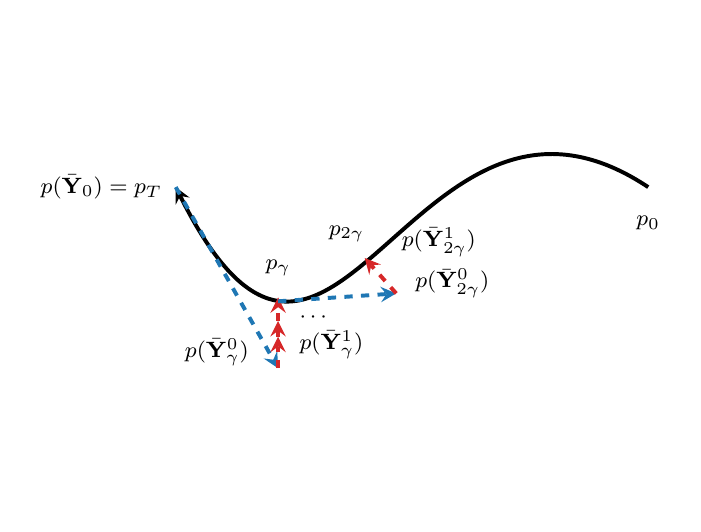
\begin{tikzpicture}
    \Large
        \draw [stealth-, line width = .05cm] (0,0) .. controls  (2,-4) and (3.,2) .. (6,0);
        \draw [-stealth, line width = .05cm, C0, dashed] (0,0) -- (1.3,-2.3);
        \draw [-stealth, line width = .05cm, C3, dashed] (1.3,-2.3) -- (1.3,-1.9);
        \draw [-stealth, line width = .05cm, C3, dashed] (1.3,-1.9) -- (1.3,-1.7);
        \draw [-stealth, line width = .05cm, C3, dashed] (1.3,-1.7) -- (1.3,-1.4);
        \draw [-stealth, line width = .05cm, C0, dashed] (1.3,-1.45) -- (2.8,-1.35);
        \draw [-stealth, line width = .05cm, C3, dashed] (2.8,-1.35) -- (2.4, -0.9);
    %   \draw [-stealth, line width = .05cm, blue, dashed] (0,0) -- (1.3,-2.3);
    %   \draw [-stealth, line width = .05cm, red, dashed] (1.3,-2.3) -- (1.3,-1.2);
    %   \draw [-stealth, line width = .05cm, blue, dashed] (1.3,-1.2) -- (2.8,-0.7);
    %   \draw [-stealth, line width = .05cm, red, dashed] (2.8,-0.7) -- (2.6, -0.5);
        \node [below=0.2cm] at (6,0) {\footnotesize $p_0$};
        \node [left=0.0cm] at (0,0) {\footnotesize $p(\bwd_0) = p_T$};
        \node [left=0.2cm] at (1.3,-2.1) {\footnotesize $p(\bwd_\gamma^0)$};
        \node [right=0.1cm] at (1.3,-2.) {\footnotesize $p(\bwd_\gamma^1)$};
        \node [right=0.1cm] at (1.3,-1.65) {\footnotesize $\cdots$};
    %   \node [below right=0.1cm] at (1.3,-1.2) {$\mathcal{L}(\fwd_\gamma^1)$};
    %   \node [above=0.05cm] at (1.3,-1.2) {$\mathcal{L}(\fwd_\gamma^3)$};
        \node [above=0.05cm] at (1.3,-1.35) {\footnotesize $p_{\gamma}$};
    %   \node [right=0.2cm] at (2.8,-0.7) {$\mathcal{L}(\fwd_{2\gamma}^0)$};
        %   \node [above left=0.1cm] at (2.6, -0.5) {$\mathcal{L}(\fwd_{2\gamma}^1)$};
        \node [below right=0.1cm] at (2.8,-0.8) {\footnotesize $p(\bwd_{2\gamma}^0)$};
        \node [right=0.1cm] at (2.6, -0.7) {\footnotesize $p(\bwd_{2\gamma}^1)$};
        \node [above left=0.05cm] at (2.6, -0.9) {\footnotesize $p_{2\gamma}$};
    \end{tikzpicture}
    }
    \end{center}
\end{figure}
\vspace{-2.cm}
{\footnotesize Credits to Valentin De Bortoli for graphic.}
\end{frame}


% \begin{frame}{Predictor-Corrector sampling}
% \vspace{-7.em}
% \begin{center}
% \begin{tikzpicture}
%   \draw [stealth-, line width = .05cm] (0,0) .. controls  (2,-4) and (4,4) .. (6,0);
%   \draw [-stealth, line width = .05cm, solidblue, dashed] (0,0) -- (1.3,-2.3);
%   \draw [-stealth, line width = .05cm, solidred, dashed] (1.3,-2.3) -- (1.3,-1.9);
%   \draw [-stealth, line width = .05cm, solidred, dashed] (1.3,-1.9) -- (1.3,-1.5);
%   \draw [-stealth, line width = .05cm, solidred, dashed] (1.3,-1.5) -- (1.3,-1.2);
%   \draw [-stealth, line width = .05cm, solidblue, dashed] (1.3,-1.2) -- (2.8,-0.7);
%   \draw [-stealth, line width = .05cm, solidred, dashed] (2.8,-0.7) -- (2.6, -0.5);
% %   \draw [-stealth, line width = .05cm, blue, dashed] (0,0) -- (1.3,-2.3);
% %   \draw [-stealth, line width = .05cm, red, dashed] (1.3,-2.3) -- (1.3,-1.2);
% %   \draw [-stealth, line width = .05cm, blue, dashed] (1.3,-1.2) -- (2.8,-0.7);
% %   \draw [-stealth, line width = .05cm, red, dashed] (2.8,-0.7) -- (2.6, -0.5);
%   \node [below=0.2cm] at (6,0) {$p_{\textrm{data}}$};
%   \node [left=0.3cm] at (0,0) {$\mathcal{L}(\bwd_0) = p_T$};
%   \node [below=0.2cm] at (1.3,-2.3) {$\mathcal{L}(\bwd_\gamma^0)$};
%   \node [right=0.1cm] at (1.3,-1.9) {$\mathcal{L}(\bwd_\gamma^1)$};
%   \node [right=0.1cm] at (1.3,-1.5) {$\cdots$};
% %   \node [below right=0.1cm] at (1.3,-1.2) {$\mathcal{L}(\bwd_\gamma^1)$};
% %   \node [above=0.05cm] at (1.3,-1.2) {$\mathcal{L}(\bwd_\gamma^3)$};
%   \node [above=0.05cm] at (1.3,-1.2) {$p_{\gamma}$};
% %   \node [right=0.2cm] at (2.8,-0.7) {$\mathcal{L}(\bwd_{2\gamma}^0)$};
%     %   \node [above left=0.1cm] at (2.6, -0.5) {$\mathcal{L}(\bwd_{2\gamma}^1)$};
%   \node [below right=0.1cm] at (2.8,-0.7) {$\mathcal{L}(\bwd_{2\gamma}^0)$};
%   \node [right=0.1cm] at (2.6, -0.5) {$\mathcal{L}(\bwd_{2\gamma}^1)$};
%   \node [above left=0.05cm] at (2.6, -0.5) {$p_{2\gamma}$};
% \end{tikzpicture}
% \end{center}
% \vspace{-2.5em}
% % \caption{
%     % Illustration of the effect of the corrector step on SGM.
%     The black line corresponds to the dynamics of the noising process 
%   $(p_t)_{t \in \ccint{0,T}}$. The \textcolor{solidblue}{blue dashed lines} correspond to the
%   predictor step (going backward in time) and the \textcolor{solidred}{red dashed lines} correspond to
%   the corrector step (projecting back onto the forward dynamics).
% %   Note that
% %   $\mathcal{L}(X_1^\gamma) \approx p_{T- \gamma}$ and
% %   $\mathcal{L}(X_2^\gamma) \approx p_{T- 2\gamma}$.
% % }

% \end{frame}
  

% \begin{frame}{Predictor-Corrector sampling from the backwards process}
% %
% \begin{algorithm}[H]
% % \caption{\small GRW-c (Geodesic Random Walk with corrector)}
% \caption{\small Predictor-Corrector}
% \label{alg:grw-c}
% \begin{algorithmic}[1]
%  \small
% %   \Require $T, N, \gamma = T / N, X_0, b, \sigma, \mathrm{P}$
% %   \Require $T, N, \gamma = T / N, X_0, b, \beta_t$
%     \Require $\bwd_0$, $T$, $N$, $S$, $\gamma = T/N$, $\gamma_{s}$
% %   \State $\gamma = T / N$ \Comment Step-size
%   \For{\textcolor{solidblue}{$k \in \{0, \dots, N-1\}$}}
%   \State \textcolor{solidblue}{/// PREDICTOR STEP}
%   \State \textcolor{solidblue}{${\bfZ}_{k+1} \sim \mathrm{N}(0, \Id)$} \Comment Standard Gaussian noise% in ambient space $\rset^p$
% %   \State \textcolor{solidblue}{$Z_{k+1/2} = \mathrm{P}(X_k^\gamma) \bar{Z}_{k+1/2}$} \Comment Projection in the tangent space $\mathrm{T}_x \M$ 
% %   \State \textcolor{solidblue}{$W_{k+1} = \gamma b(k \gamma, X_k) + \sqrt{\gamma} \sigma(k \gamma, X_k) Z_{k+1}$} \Comment Euler--Maruyama step %on tangent space 
% %   \State \textcolor{solidblue}{$W_{k+1} = \gamma b(k \gamma, X_k) + \sqrt{\gamma} \sigma(k \gamma, X_k) Z_{k+1}$} \Comment Euler--Maruyama step %on tangent space 
%   \State \textcolor{solidblue}{$\bwd_{k+1} = \bwd_{k} + \gamma \sbr{-b(T-k \gamma, \bwd_k) + \nabla \log p_{T-k\gamma}(\bwd_{k})} + \sqrt{\gamma} \bfZ_{k+1}$} \Comment E-M step %on tangent space 
% %   \State \textcolor{solidblue}{$X_{k+1} = \exp_{X_k}[W_{k+1}]$} \Comment %Geodesic projection onto $\M$

%   \State \textcolor{solidred}{/// CORRECTOR STEP}
%   \State \textcolor{solidred}{${\bwd}_{k+1}^0 = {\bwd}_{k+1}$}
%   \For{\textcolor{solidred}{$s \in \{0, \dots, S-1\}$}}
%   \State \textcolor{solidred}{${\bfZ}_{k+1}^s \sim \mathrm{N}(0, \Id)$} \Comment Standard Gaussian noise% in ambient space $\rset^p$
% %   \State \textcolor{solidred}{$Z_{k+1} = \mathrm{P}(X_{k+1/2}^\gamma) \bar{Z}_{k+1}$} \Comment Projection in the tangent space $\mathrm{T}_x \M$ 
% %   \State \textcolor{solidred}{$W_{k+1}^{l+1} = \tfrac{\gamma}{2} b(k \gamma, X_{k}^l) + \sqrt{\gamma} \sigma(k \gamma, X_{k}^l) Z_{k+1}$} \Comment Euler--Maruyama step% on tangent space \label{line:dete}
%   \State \textcolor{solidred}{$\bwd_{k+1}^{s+1} = \bwd_{k+1}^{s} + \gamma_s \nabla \log p_{T-k\gamma}(\bwd_{k+1}^{s}) + \sqrt{2 \gamma_s} \bfZ_{k+1}^s$} \Comment Langevin step% on tangent space \label{line:dete}
% %   \State \textcolor{solidred}{$X_{k+1}^{l+1} = \exp_{X_{k}^l}[W_{k+1}^{l+1}]$} \Comment %Geodesic projection onto $\M$  
%   \EndFor
%   \State \textcolor{solidred}{${\bwd}_{k+1} = {\bwd}_{k+1}^S$}
%   \EndFor
%   \State {\bfseries return} $\bwd_N$
% \end{algorithmic}
% \end{algorithm}

    
% \end{frame}

% \begin{frame}{Important 'tricks' - The SDE}
    
% % \todo[inline]{Also: Loss function weighting, corrector and more}

% \textbf{Noise scheduling}:
% For whatever SDE we are looking at, remap
% \begin{itemize}
%     \item $\hlblue{b(t, \fwd_{t})} \to \beta(t) \hlblue{b(t, \fwd_{t})}$
%     \item $\hlred{\sigma(t)} \to \sqrt{\beta(t)} \hlred{\sigma(t)}$
% \end{itemize}
% Doing this is equivalent to \textit{re-scaling time} such that $t \mapsto \int_0^t \beta(s) ds$. We can set $\beta(t)$ to reduce the step size where the score norm is high.

% % The aim is to have a linear convergence $\mathbb{W}(\mathcal{L}(\fwd_t), \piinv) \approx \mathbb{W}(\mathcal{L}(\fwd_t), p_0) * (1 - t)_+$ of the discrete steps from reference measure to data.

% \pause

% \textbf{Process truncation}: As $t \to 0$, the score blows up, i.e.\ $\|\hlyellow{\nabla \log p(x_t)}\| \rightarrow \infty$, with the manifold hypothesis~\cite{debortoli2022Convergence}, or we only have access to finite data.
% % or since finite data gives a product of Dirac masses distribution.


% Truncating the process so that $t \in \sbr{\epsilon, T}$ prevents this issue.
% % This is equivalent to adding a small amount of the noise to the data, and puts density everywhere.
% This is equivalent to smoothing the data with some small noise, effectively extending the support of the data distribution to $\rset^d$.
% % adding a small amount of the noise to the data, and puts density everywhere.


% % \begin{itemize} \setbeamertemplate{itemize items}[triangle]
% %     \item \textbf{Noise scheduling} $\beta(t)$
% %     \begin{itemize} \setbeamertemplate{itemize items}[circle]
% %     \item $\rmd \fwd_t = \hlblue{-\beta(t)~\fwd_t} \rmd t + \hlred{\sqrt{2 \beta(t)}} \rmd \bfB_t$.
% %     \item `Rescale time': $t \mapsto \int_0^t \beta(s) ds$.
% %     \item Spend more time when the score has high norm, i.e.\ when $t$ is small.
% %     \item Aim: linear rate of convergence, i.e.\ $\mathbb{W}(\mathcal{L}(\fwd_t), \piinv) \approx \mathbb{W}(\mathcal{L}(\fwd_t), p_0) * (1 - t)$.
% %     % \item Aim: $\mathbb{W}(\mathcal{L}(\fwd_t), \piinv)$ roughly linear with $t$ and $\approx 0$ when $t=1$.
% %     \end{itemize} \setbeamertemplate{itemize items}[triangle]
% %     \item Truncate processes between $[\epsilon, T]$ with $\epsilon > 0$ since $\|\nabla \log p(x_t)\| \rightarrow \infty$ as $t \rightarrow 0$ with manifold hypothesis~\cite{debortoli2022Convergence}.
% %     \item \textbf{Loss weighting} $\lambda(t)$
% %     \begin{itemize} \setbeamertemplate{itemize items}[circle]
% %         \item $\lambda(t) \propto 1/ \PE{\left[\|\nabla \log p_{0|t}(x_t|x_0) \|^2\right]} \Rightarrow$ focus on small $t$~\cite{song2020improved}.
% %         \item $\lambda(t) = 2 \beta(t) \Rightarrow$ 'likelihood weighting'~\cite{song2021maximum,huang2021variational}.
% %     \end{itemize}
% %     \item \textbf{Exponential moving average} of the weights $\theta$ at evaluation due to high stochasticity of the training loss.
% % \end{itemize}
    
% \end{frame}


% \begin{frame}{Important 'tricks' - Learning the score}
% \textbf{Parametrising the score}: Learning the score naively can prove tricky. There is a principled way to parameterise the score however!
% \begin{align*}
%     \rmd \bwd_t = \sbr{-\hlblue{b(T-t, \bwd_t)} + \hlred{\sigma(T-t)}^2 \hlyellow{\v{s}_\theta}(T-t, \bwd_t)}\rmd t +  \hlred{\sigma(T-t)} \rmd \bfB_t
% \end{align*}
% We set
% \begin{equation*}
%     \hlyellow{\v{s}_\theta}(t, \bwd_t) = \v{h}_\theta(t, \bwd_t) / \sigma_t + {2\hlblue{b(t, \bwd_t)}}/{\hlred{\sigma(t)}^2}, \quad \sigma_t = \PE{\left[ \| \nabla \log p(\fwd_t|\fwd_0)\|^2 \right]}^{1/2}.
% \end{equation*}
% \vspace{-\topsep}
% \begin{enumerate}
%     \item This sets the dynamics of the backwards SDE to be the same as the forward if $\v{h}_\theta(t, \bwd_t) = 0$.
%     \item This normalises $\v{h}_\theta(t, \bwd_t)$ to have expected norm of 1.
% \end{enumerate}
% We can show that $\PE{\left[ \| \nabla \log p(\fwd_t|\fwd_0)\|^2 \right]}^{1/2} = \text{Std}[\fwd_t|\fwd_0] = \sigma_t$.
% % This is something we can typically compute for a known SDE.
% %
% % \begin{itemize} \setbeamertemplate{itemize items}[triangle]
% %     \item \textbf{Score network parametrisation}
% %     \begin{itemize} \setbeamertemplate{itemize items}[circle]
% %         \item $\rmd \bwd_t = \hlblue{\left[-b(t, \bwd_t) + 2 \beta(t) \mathbf{s}_\theta(t, \bwd_t) \right]} \rmd t + \hlred{\sqrt{2\beta(t)}} \rmd \bfB_t$.
% %         \item $\hlyellow{\mathbf{s}_\theta}(t, y_t) = \left(h_\theta(t, y_t)/ \sigma_t + 2 * \hlblue{b(t, y_t)}/\beta(t) \right)$.
% %         \item $\rmd \bwd_t = \hlblue{\left[b(t, \bwd_t) + 2 \beta(t) \mathbf{h}_\theta(t, \bwd_t) / \sigma_t \right]} \rmd t + \hlred{\sqrt{2\beta(t)}} \rmd \bfB_t$.
% %         \item If $h_\theta(t, x_t)=0 \Rightarrow \rmd \bwd_t = \rmd \fwd_{t}$.
% %         % \item $\hlyellow{\mathbf{s}_\theta}(t, x_t) = \left(h_\theta(t, x_t)/ \sigma_t + 2*\hlblue{b(t, x_t)}/\beta(t) \right)$.
% %         \item With $\sigma_t \triangleq \PE{\left[ \| \nabla \log p(\fwd_t|\fwd_0)\|^2 \right]}^{1/2} = \text{Std}[\fwd_t|\fwd_0] = 1 - e^{-\int_0^t \beta(s) ds}$.
% %         % \begin{itemize}
% %             \item $1/\sigma_t\rightarrow 0$ as $t\rightarrow \infty$ and $1/\sigma_t \rightarrow \infty$ as $t \rightarrow 0$.
% %         % \end{itemize}
% %         % \item with $\PE{\left[ \| \nabla \log p(\fwd_t|\fwd_0)\|^2 \right]}^{1/2} = \text{Std}[\fwd_t|\fwd_0] \triangleq \sigma_t = 1 - e^{-\int_0^1 \beta(s) ds}$.
% %         % % \item Such that if $h_\theta(t, x_t)=0$, reverse drift $\bar{b}(t, y_t) = -\beta(t) b(t, x_t) + \beta(t) * 2*b(t, x_t)/\beta(t) ={b}(t, y_t)$.
% %         % \item If $h_\theta(t, x_t)=0$, \textbf{forward=backward} since $\hlblue{\bar{b}(t, y_t) = {b}(t, y_t)}$.
% %         % % \item and $\hlblue{b}$ forward drift ($\hlblue{b(t, x_t)}/\beta(t)^2 = -x_t$ if $\M = \rset^d$).
% %         % \item If $\M=\rset$ recovers more or less \cite[][e.g.]{daras2022Soft} [Not exactly as they use $\sigma^2$?].
% %     \end{itemize}
    
% % \end{itemize}
% \end{frame}

% \begin{frame}{Important 'tricks' - Learning the score}
%     The denoising score matching loss has high variance when approximated with Monte Carlo.

%     $\implies$ Using a exponential moving average of the parameters at test time is very impactful.
% \end{frame}




% \section{Likelihood evaluation and connection with continuous normalising flows}

% \begin{frame}{Probability flow}
% \begin{frame}{Likelihood evaluation}
% %
% % \vspace{-0.5em}
% %
% Given the SDE $\rmd \fwd_t = \hlblue{b(t, \fwd_t)} \rmd t + \hlred{\Sigma^{1/2}(t, \fwd_t)} \rmd \bfB_t$, the
% % \begin{equation}
% % \label{eq:}
% % \end{equation}
% \textbf{Fokker-Planck} equation describes the evolution of the density
% \begin{equation}
% \label{eq:fokker_planck}
% \frac{\partial}{\partial t} p_t(x) = -\dive\left( \hlblue{b(t, \cdot)} p_t(\cdot) \right)(x) + \frac{1}{2} \sum_{i,j} \frac{\partial^2}{\partial_i\partial_j} \left( \hlred{\Sigma_{i,j}(t, \cdot)} p_t(\cdot) \right)(x).
% \end{equation}
% \pause
% \vspace{-\topsep}
% \begin{itemize}
%     \setbeamertemplate{itemize items}[triangle]
%     \item If $\hlred{\Sigma = 0}$ (deterministic dynamics): 
% \end{itemize}
% \begin{equation*}
%     \frac{\partial}{\partial t} p_t(x) = -\dive\left( \hlblue{b(t, \cdot)} p_t(\cdot)  \right) (x).
% \end{equation*}
% \pause
% \vspace{-\topsep}
% \begin{itemize} \setbeamertemplate{itemize items}[triangle]
%     \item If $\hlred{\Sigma = \sigma^2(t) \m{I}}$ (Langevin dynamics):
% \end{itemize}
% \vspace{-0.5em}
% \begin{align*}
% \label{eq:fokker_planck_isotropic}
% \frac{\partial}{\partial t} p_t(x) 
% &= -\dive\left( \hlblue{b(t, \cdot)} p_t(\cdot)  \right)(x)  + \tfrac{1}{2} \hlred{\sigma(t)}^2 \Delta p_t (x) \\
% &= -\dive\left( \left[ \hlblue{b(t, \cdot)} - \tfrac{1}{2} \hlred{\sigma(t)}^2 \hlyellow{\nabla \log p_t(\cdot)} \right] p_t(x)  \right).
% \end{align*}
% %
% \end{frame}

% \begin{frame}{Likelihood evaluation (Cont'd)}
% % Since we can express the evolution of the density of the SDE 
% % % $\rmd \fwd_t = \hlblue{b(t, \fwd_t)} \rmd t + \hlred{\Sigma^{1/2}(t, \fwd_t)} \rmd \bfB_t$ 
% % $\rmd \fwd_t = \hlblue{b(t, \fwd_t)} \rmd t + \hlred{\sigma(t)} \rmd \bfB_t$ 
% % in the same fashion as for the deterministic dynamics
% % \begin{equation*}
% %     \frac{\partial}{\partial t} p_t(x) = -\dive\left( \left[ \hlblue{b(t, \cdot)} - \tfrac{1}{2}\hlred{\sigma(t)}^2 \hlyellow{\nabla \log p_t(\cdot)} \right] p_t(\cdot) \right) (x).
% % \end{equation*}
% % \pause
% Then both of the following dynamics
% \begin{enumerate}
%     \item $\rmd \fwd_t = \hlblue{b(t, \fwd_t)} \rmd t + \hlred{\sigma(t)} \rmd \bfB_t$ (stochastic).
%     \item $\rmd \fwd_t = \left[ \hlblue{b(t, \fwd_t)} - \tfrac{1}{2} \hlred{\sigma(t)}^2 \hlyellow{\nabla \log p_t(\fwd_t)} \right] \rmd t$ (deterministic).
% \end{enumerate}
% have the same marginal density $\Pbb_t\triangleq\c{L}(\fwd_t)$ which evolution is given by
% \begin{equation*}
%     \frac{\partial}{\partial t} p_t(x) = -\dive\left( \left[ \hlblue{b(t, \cdot)} - \tfrac{1}{2}\hlred{\sigma(t)}^2 \hlyellow{\nabla \log p_t(\cdot)} \right] p_t(\cdot) \right) (x).
% \end{equation*}
% This gives us a \textit{deterministic} ODE with the same marginal density as the SDE.
% % probability density as the SDE.
% %
% \begin{center}
%     \includegraphics[width=0.8\textwidth]{images/sde.png}
% \end{center}
% %
% \end{frame}

% \begin{frame}{Log-likelihood evolution of ODEs}
% %
% \vspace{-0.5em}
% %
% Assume \textbf{deterministic} evolution of $\fwd_t$ given by the ODE
% \begin{equation}
%     \rmd \fwd_t = \hlblue{b(t, \fwd_t)} \rmd t.
% \end{equation}
% %
% The associated \textbf{Fokker-Planck} equation is
% \begin{equation}
%   \frac{\partial}{\partial t} p_t(\fwd_t) = -\dive\left( \hlblue{b(t, \cdot)} p_t(\cdot) \right) (\fwd_t).
% \end{equation}
% \pause
% %
% The evolution of the log-density is
% \begin{equation}
%   \frac{\partial}{\partial t} \log p_t(x) = -\dive\left( \hlblue{b(t, \cdot)} \right) (x) - \langle \hlblue{b(t, \cdot)}, \nabla \log p_t(x) \rangle.
% \end{equation}
% \pause
% %
% Combining the two dynamics
% \begin{equation}
%   \frac{\rmd}{\rmd t} \log p_t(x) = -\dive\left( \hlblue{b(t, \cdot)} \right) (x).
% \end{equation}
% % \begin{align}
% %     \frac{\rmd}{\rmd t} p_t(\fwd_t) 
% %     &= \frac{\partial}{\partial t} p_t(\fwd_t) + \langle \frac{\partial}{\partial x} p_t(\fwd_t), \frac{\partial}{\partial t} \fwd_t \rangle \\
% %     &= -\dive\left( \hlblue{b(t, \cdot)} p_t \right) (\fwd_t) + \langle \frac{\partial}{\partial x} p_t, \hlblue{b(t, \cdot)} \rangle(\fwd_t) \\
% %      &= -p_t(\fwd_t) ~\dive\left( \hlblue{b(t, \cdot)}\right) (\fwd_t) - \langle \frac{\partial}{\partial x} p_t, \hlblue{b(t, \cdot)} \rangle(\fwd_t) + \langle \frac{\partial}{\partial x} p_t, \hlblue{b(t, \cdot)} \rangle(\fwd_t) \\
% %       \frac{\rmd}{\rmd t} \log p_t(\fwd_t) &= \dive\left( \hlblue{b(t, \cdot)}\right) (\fwd_t).
% % \end{align}
% %
% The \textbf{log-likelihood} can be computed as
% \begin{equation}
%     \log p_0(\fwd_0) = \log p_T(\fwd_T) + \int_0^T  \dive \left( \hlblue{b(t, \cdot)} \right)(\fwd_t) \rmd t.
% \end{equation}

% \end{frame}

% \begin{frame}{Log-likelihood evolution of ODEs}
% %
% \vspace{-0.5em}
% %
% Assume a \textbf{deterministic} evolution of $\fwd_t$ given by the ODE
% \begin{equation}
%     \rmd \fwd_t = \hlblue{b(t, \fwd_t)} \rmd t.
% \end{equation}
% %
% The evolution of the log-density is given by \cite{chen2018neural}
% \begin{equation}
%   \frac{\rmd}{\rmd t} \log p_t(x) = -\dive\left( \hlblue{b(t, \cdot)} \right) (x).
% \end{equation}
% \pause
% % \begin{align}
% %     \frac{\rmd}{\rmd t} p_t(\fwd_t) 
% %     &= \frac{\partial}{\partial t} p_t(\fwd_t) + \langle \frac{\partial}{\partial x} p_t(\fwd_t), \frac{\partial}{\partial t} \fwd_t \rangle \\
% %     &= -\dive\left( \hlblue{b(t, \cdot)} p_t \right) (\fwd_t) + \langle \frac{\partial}{\partial x} p_t, \hlblue{b(t, \cdot)} \rangle(\fwd_t) \\
% %      &= -p_t(\fwd_t) ~\dive\left( \hlblue{b(t, \cdot)}\right) (\fwd_t) - \langle \frac{\partial}{\partial x} p_t, \hlblue{b(t, \cdot)} \rangle(\fwd_t) + \langle \frac{\partial}{\partial x} p_t, \hlblue{b(t, \cdot)} \rangle(\fwd_t) \\
% %       \frac{\rmd}{\rmd t} \log p_t(\fwd_t) &= \dive\left( \hlblue{b(t, \cdot)}\right) (\fwd_t).
% % \end{align}
% %
% Assuming that $\fwd_T \sim p_T$, the \textbf{log-likelihood} can be computed as
% \begin{equation}
%     \log p_0(\fwd_0) = \log p_T(\fwd_T) + \int_0^T  \dive \left( \hlblue{b(t, \cdot)} \right)(\fwd_t) \rmd t.
% \end{equation}
% \end{frame}

% \begin{frame}{Log-likelihood evaluation of ODEs}
% % We can't solve this log-likelihood computation exactly, instead we need to solve the \textbf{augmented ODE}
% The following \textbf{augmented ODE} allows to solve at once the trajectory of $\fwd_t$ and the change in log-likelihood
% \begin{equation}
%     \frac{\rmd}{\rmd t} 
%     \begin{bmatrix} \fwd_t \\ \log p(\fwd_t) \end{bmatrix}
%     = {\begin{bmatrix} \hlblue{b_\theta(t, \cdot)} \\ -\dive\left(\hlblue{b_\theta(t, \cdot)} \right) \end{bmatrix}(\fwd_t)}.
% \end{equation}
% % Which we can do with a myriad of ODE solvers, many of which come with \textit{controllable error}!
% Which can be estimated numerically with a myriad of (adaptive) ODE solvers.
% \pause

% % This is exactly how \textbf{Neural ODEs} \cite{chen2018neural,grathwohl2019Scalable} are trained.
% This is exactly how \textbf{continuous normalising flows} \cite{chen2018neural,grathwohl2019Scalable} are trained.
% Maximising the likelihood ($\c{O}(Nd^2)$ or $\c{O}(Nd)$ with $\dive$ estimator)
% \begin{equation}
%     % {\scriptstyle
%     \PE \left[ \log p_0(\fwd_0) \right] = \PE [  \log p_T(\fwd_T) - \int_0^T \dive( \hlblue{b_\theta(t, \fwd_t)}) \rmd t ].
%     % }
% \end{equation}
% %
% % The 
% % vs \textbf{discrete} normalising flows with invertible map $f_\theta:\rset^d \rightarrow \rset^d$ ($\c{O}(d^3)$)
% % \begin{equation}
% % \PE \left[ \log p_0(\fwd_0) \right] = \PE \left[  \log p_T(f_\theta(\fwd_0)) - \log |\mathrm{D} f_\theta(\fwd_0)|  \right].
% % \end{equation}
% \end{frame}

% \begin{frame}{Probability flow \cite{song2021Scorebased}}
% %
% % We can apply this ODE method directly to our SDEs by converting to the ODE form, and plugging it in! The SDE
% We can apply this likelihood evaluation method for continuous SGMs induced by% the SDE
% \begin{equation}
%   \rmd \fwd_t = \hlblue{\hlblue{b(t, \fwd_t)}} \rmd t + \hlred{\sigma(t)} \rmd \bfB_t
% \end{equation}
% % has the ODE
% since it has the same marginal density has the ODE
% \begin{equation*}
%     \rmd \fwd_t = \left[ \hlblue{b(t, \fwd_t)} - \tfrac{1}{2} \hlred{\sigma(t)}^2 \hlyellow{\nabla \log p_t(\fwd_t)} \right] \rmd t.
% \end{equation*}
% \pause
% % So we can compute the log-likelihood exactly the same way as with the ODEs, by solving the augmented ODE
% We have the associated augmented ODE
% \begin{equation}
%     \frac{\rmd}{\rmd t} 
%     \begin{bmatrix} \fwd_t \\ \log p(\fwd_t) \end{bmatrix}
%     = {\begin{bmatrix} \hlblue{b(t, \fwd_t)} - \tfrac{1}{2} \hlred{\sigma(t)}^2 \hlyellow{\nabla \log p_t(\fwd_t)} \\ 
%     -\dive\left(\hlblue{b(t, \fwd_t)} - \tfrac{1}{2} \hlred{\sigma(t)}^2 \hlyellow{\nabla \log p_t(\fwd_t)}\right) \end{bmatrix}(\fwd_t)}.
% \end{equation}
% We then just have to add on the log likelihood of the reference density, $\log p_T(\fwd_T)$.
% % \begin{equation}
% % %   \rmd \bwd_t = \hlblue{\left[  \bwd_t + 2 \nabla \log p_{T-t}(\bwd_t)\right] } \rmd t + \hlred{\sqrt{2}} \rmd \bfB_t.
% %   \rmd \bwd_t = \hlblue{\left[ -\hlblue{b(T-t, \bwd_t)} + 2 \nabla \log p_{T-t}(\bwd_t)\right] } \rmd t + \hlred{\sqrt{2}} \rmd \bfB_t.
% % \end{equation}
% % \pause
% % %
% % ${\bwd}_t$ has the same distribution as $\hat{\bwd}_t$ with \textbf{determinisitic} dynamics given by the ODE
% % \begin{equation}
% % %   \rmd \hat{\bwd}_t = \hlblue{\left[  \bwd_t + \nabla \log p_{T-t}(\bwd_t)\right] } \rmd t
% %   \rmd \hat{\bwd}_t = \hlblue{\left[ -\hlblue{b(T-t, \bwd_t)} + \nabla \log p_{T-t}(\bwd_t)\right] } \rmd t
% % \end{equation}
% % % since for both ${\bwd}_t$ and $\hat{\bwd}_t$ we have that
% % since they have the same density evolution:
% % \begin{align}
% %   \frac{\partial}{\partial t} \log p_t({\bwd}_t) 
% % %   &= -\dive\left( \hlblue{b(t, \cdot)} p_t \right) ({\bwd}_t) + \tfrac{\hlred{2}}{2} \Delta p_t ({\bwd}_t) \\
% % %   &= -\dive\left( \hlblue{\left[ b(t, \cdot) - \nabla \log p_t \right]} p_t \right) (\hat{\bwd}_t)
% %   &= -\dive\left( \hlblue{\left[-b(T-t, \cdot) + 2 \nabla \log p_{T-t} \right]} p_t \right) ({\bwd}_t) + \tfrac{\hlred{\sqrt{2}}^2}{2} \Delta p_t ({\bwd}_t) \\
% %   &= -\dive\left( \hlblue{\left[ -b(T-t, \cdot) + \nabla \log p_{T-t} \right]} p_t \right) (\hat{\bwd}_t)
% %   = \frac{\partial}{\partial t} \log p_t(\hat{\bwd}_t).
% % \end{align}
% % = 
% % = -\dive\left( \left[ \hlblue{b(t, \cdot)} - \tfrac{\hlred{c}}{2} \nabla \log p_t \right] p_t \right) (x)
%
% \end{frame}


% \begin{frame}{Probability flow \cite{song2021Scorebased}}
% %
% The continuous time reversal process of the forward process
% \begin{equation}
%   \rmd \fwd_t = \hlblue{\hlblue{b(t, \fwd_t)}} \rmd t + \hlred{\sqrt{2}} \rmd \bfB_t
% \end{equation}
% is given by
% \begin{equation}
% %   \rmd \bwd_t = \hlblue{\left[  \bwd_t + 2 \nabla \log p_{T-t}(\bwd_t)\right] } \rmd t + \hlred{\sqrt{2}} \rmd \bfB_t.
%   \rmd \bwd_t = \hlblue{\left[ -\hlblue{b(T-t, \bwd_t)} + 2 \nabla \log p_{T-t}(\bwd_t)\right] } \rmd t + \hlred{\sqrt{2}} \rmd \bfB_t.
% \end{equation}
% \pause
% %
% ${\bwd}_t$ has the same distribution as $\hat{\bwd}_t$ with \textbf{determinisitic} dynamics given by the ODE
% \begin{equation}
% %   \rmd \hat{\bwd}_t = \hlblue{\left[  \bwd_t + \nabla \log p_{T-t}(\bwd_t)\right] } \rmd t
%   \rmd \hat{\bwd}_t = \hlblue{\left[ -\hlblue{b(T-t, \bwd_t)} + \nabla \log p_{T-t}(\bwd_t)\right] } \rmd t
% \end{equation}
% % since for both ${\bwd}_t$ and $\hat{\bwd}_t$ we have that
% since they have the same density evolution:
% \begin{align}
%   \frac{\partial}{\partial t} \log p_t({\bwd}_t) 
% %   &= -\dive\left( \hlblue{b(t, \cdot)} p_t \right) ({\bwd}_t) + \tfrac{\hlred{2}}{2} \Delta p_t ({\bwd}_t) \\
% %   &= -\dive\left( \hlblue{\left[ b(t, \cdot) - \nabla \log p_t \right]} p_t \right) (\hat{\bwd}_t)
%   &= -\dive\left( \hlblue{\left[-b(T-t, \cdot) + 2 \nabla \log p_{T-t} \right]} p_t \right) ({\bwd}_t) + \tfrac{\hlred{\sqrt{2}}^2}{2} \Delta p_t ({\bwd}_t) \\
%   &= -\dive\left( \hlblue{\left[ -b(T-t, \cdot) + \nabla \log p_{T-t} \right]} p_t \right) (\hat{\bwd}_t)
%   = \frac{\partial}{\partial t} \log p_t(\hat{\bwd}_t).
% \end{align}
% % = 
% % = -\dive\left( \left[ \hlblue{b(t, \cdot)} - \tfrac{\hlred{c}}{2} \nabla \log p_t \right] p_t \right) (x)

% \end{frame}


% \begin{frame}{Continuous normalising flows (CNFs) ~\cite{chen2018neural,grathwohl2019Scalable}}
% %
% Assume \textbf{deterministic} forward evolution of $\fwd_t$ with dynamics given by the ODE
% \begin{equation}
%     \rmd \fwd_t = \hlblue{b_\theta(t, \fwd_t)} \rmd t
%     \quad \text{thus a backward evolution} \quad \rmd \bwd_t = \hlblue{b_\theta(T - t, \bwd_t)} \rmd t
% \end{equation}
% where $\hlblue{b_\theta}: \rset_+ \times \rset^d \rightarrow \rset^d$ is a parametric family of drifts (i.e.\ vector fields). 
% \pause
% %

% Consider the \textbf{augmented} ODE
% \begin{equation}
%     \frac{\rmd}{\rmd t} 
%     \begin{bmatrix} \fwd_t \\ \log p(\fwd_t) \end{bmatrix}
%     = \hlblue{\begin{bmatrix} b_\theta(t, \cdot) \\ -\dive\left(b_\theta(t, \cdot) \right) \end{bmatrix}(\fwd_t)}.
% \end{equation}
% \pause
% %
% Train drift \hlblue{b_\theta} by maximising the likelihood ($\c{O}(Nd^2)$ or $\c{O}(Nd)$ with $\dive$ estimator)
% \begin{equation}
%     % {\scriptstyle
%     \PE \left[ \log p_0(\fwd_0) \right] = \PE [  \log p_T(\fwd_T) - \int_0^T \dive( \hlblue{b_\theta(s, \fwd_s)}) \rmd s ].
%     % }
% \end{equation}
% %
% % The 
% vs \textbf{discrete} normalising flows with invertible map $f_\theta:\rset^d \rightarrow \rset^d$ ($\c{O}(d^3)$)
% \begin{equation}
% \PE \left[ \log p_0(\fwd_0) \right] = \PE \left[  \log p_T(f_\theta(\fwd_0)) - \log |\mathrm{D} f_\theta(\fwd_0)|  \right].
% \end{equation}
% \end{frame}


\begin{frame}{Recap: Continuous diffusion models}
 %
 \begin{center}
        \includegraphics[width=\textwidth]{images/sde.png}
    \end{center}
\begin{itemize} \setbeamertemplate{itemize items}[triangle]
    \item Continuously \textbf{noise} data samples with forward SDE
    \item Aim: time-reversal of this process $\Rightarrow$ \textbf{denoising} process
    % \begin{itemize} \setbeamertemplate{itemize items}[circle]
    % \item Same variance as the forward process
    % \item Its mean depends on the forward process's mean and the \textbf{Stein score}
    % \item The score is parametrised and trained by learning to `denoise' samples
    % \item Generate samples by discretising the (approximate) backward process with Euler-Maruyama
    % \end{itemize}
\end{itemize}
%
% \begin{itemize}
%     \item Idea: Use a \textit{continuous} series of noise scales!
%     \item Do this by constructing an \textbf{SDE} forward noising process $(\fwd_t)_{t \in \ccint{0,T}}$.
%     \item Have this noising converge to a \textbf{known distribution}.
%     \item \textbf{Invert} this SDE noising process to get $(\bwd_t)_{t\in[0,T]} = (\fwd_{T-t})_{t}$.
% \end{itemize}
\end{frame}

% \section{A variational perspective}

% % \begin{frame}{Equivalence between SM and ELBO loss}
% % \begin{frame}{Discrete SGMs}

% % \todo[inline]{To fill}
% % \cite{sohl2015deep,ho2020denoising,nichol2021improved}
% % \end{frame}


% \begin{frame}{Discrete SGMs: ELBO \cite{sohl2015deep,ho2020denoising}}
% %
% We assume a discrete process induced by the \textbf{forward transition} $q(\v{y}_{t}|\v{y}_{t-1})$:
%     % $p_{k+1|k}(\v{y}_{k+1}|\v{y}_{k})$ (e.g.\ $\c{N}(\mu_k(\v{y}_k), \sigma_k)$
%      % (e.g.\ $\c{N}(\mu_k(\v{y}_t), \sigma_t)$)
% %
%     \begin{equation}\label{eq:forward_markov}
%          q(\v{y}_{0:T}) = q(\v{y}_0) \prod_{t=1}^{T} q(\v{y}_{t}|\v{y}_{t-1}).
%     \end{equation}
% %
% The (intractable) \textbf{backward transition} $p_{t-1|t}(\v{y}_{t-1}|\v{y}_{t})$ 
% % $p_{t|t+1}(\v{y}_{t}|\v{y}_{t+1}) = p_{t+1|t}(\v{y}_{t+1}|\v{y}_{t}) p_{t}(\v{y}_{t})/ p_{t+1}(\v{y}_{t+1})$ 
% induces a backward process% given by the Markov chain
% % For Gaussian forward process, the \textbf{backwards process}, $p(x_{t-1}|x_{t})$, is also (approximately, for sufficiently small steps) Gaussian with intractable mean and closed-form variance, yielding
%     % \begin{equation}\label{eq:backward_markov}
%     %     p(x_{0:N}) = p(x_N) \prod_{k=0}^{N-1} p_{k|k+1}(x_{k}|x_{k+1}).
%     % \end{equation}
%     \begin{equation}\label{eq:backward_markov}
%         p({\v{y}}_{0:T}) = p({\v{y}}_T) \prod_{t=T}^{1} p({\v{y}}_{t-1}|{\v{y}}_{t}).%, \quad p({x}_{t-1}|{x}_{t}) \approx \c{N}\del{{x}_{t-1}\middle| \v{\mu}\del{{x}_t, t}, \m{\Sigma}_t}.
%     \end{equation}
%     \pause
%     %
%     % But how do we \textbf{train} an approximate mean function ${\v{\mu}_\theta}\del{\v{y}_t, t}$?
% A bound on the (negative) \textbf{log-likelihood} can be derived as
%     \begin{align*}
%         \E\sbr{-\log p_\theta(\v{y}_0)} \leq \E_q\sbr{- \log \frac{p_\theta(\v{y}_{0:T})}{q(\v{y}_{1:T}|\v{y}_0)}} = \E_q \sbr{ -\log p(\v{y}_T) - \sum_{t \geq 1}\log \frac{p_\theta(\v{y}_{t-1}| \v{y}_{t})}{q(\v{y}_t | \v{y}_{t-1})}}
%         \triangleq \c{E}
%         % \log p_\theta({x_0}) &\geq \E_{q({x}_{1:T}|{x}_0)}\sbr{\log \frac{p_\theta({x}_{0:T})}{q({x}_{1:T}|{x}_0)}} = \E_{q({x}_{1:T}|{x}_0)} \sbr{\log p({x}_T) + \sum_{t \geq 1}\log \frac{p_\theta({x}_{t-1}| {x}_{t})}{q({x}_t | {x}_{t-1})}} 
%         % \\ &\geq
%     \end{align*}
%     which can straightforwardly be estimated via Monte Carlo sampling.
%     % All these terms are computable, and so we could train via Monte Carlo sampling and SGD.

% \end{frame}


% \begin{frame}{A more efficient EBLO}
% %
% \vspace{-1.2em}
% \begin{equation*}
%     \c{E} = 
%     \E_q \sbr{
%         \underbrace{
%             D_{KL} \del{q(\v{y}_T | \v{y}_0) \middle| \middle| p(\v{y}_T)}
%         }_{\hlblue{\scriptstyle L_T}}
%          + \sum_{t>1} \underbrace{
%             D_{KL}\del{q(\v{y}_{t-1}| \v{y}_t, \v{y}_0)  \middle| \middle | p_\theta(\v{y}_{t-1} | \v{y}_t)}
%         }_{\hlred{\scriptstyle L_{t-1}}}
%         \underbrace{- \log p_\theta(\v{y}_0 | \v{y}_1)}_{\hlorange{\scriptstyle L_0}}
%     }.
% \end{equation*}
% \vspace{-1.0em}
% %
% \begin{itemize}
%     \item[\hlblue{L_T}] \textit{prior matching}: constant if we fix $q$
%     \item[\hlorange{L_0}] \textit{reconstruction}: can compute directly
%     \item[\hlred{L_{t-1}}] \textit{denoising matching}: requires access to $q(\v{y}_{t-1}| \v{y}_t, \v{y}_0)=q(\v{y}_{t-1}| \v{y}_0)$
% \end{itemize}
% \pause
% % These are all closed form KL divergences!
% % Fortunately we can get at this! $q(\v{y}_{t-1}| \v{y}_t, \v{y}_0) = \c{N}\del{\v{y}_{t-1} \middle | \tilde{\v{\mu}}_t\del{\v{y}_t, \v{y}_0}, \tilde{\beta}_t \m{I}}$ with
% % \begin{equation*}
% %     \tilde{\v{\mu}}_t\del{\v{y}_t, \v{y}_0} = \frac{\sqrt{1-\alpha_{t-1}} \beta_t}{\alpha_t}\v{y}_0 + \frac{\sqrt{1-\alpha_t}(\alpha_{t-1})}{\alpha_t}\v{y}_t \; \text{and} \; \tilde{\beta}_t = \frac{\alpha_{t-1}}{\alpha_t}\beta_t
% % \end{equation*}
% Denoting $\v{\mu}_q\del{x_t, x_0} = \PE[\fwd_t|\fwd_0]$ and ${\sigma}_q\del{t} = \text{Std}[\fwd_t|\fwd_0]$

% Choosing $p(\v{y}_{t-1}|\v{y}_{t}) \approx p_\theta(\v{y}_{t-1}|\v{y}_{t}) \triangleq \c{N}\del{\v{y}_{t-1}\middle| \v{\mu}_\theta \del{t, \v{y}_t}, \sigma^2_q(t) \Id}$ we have
% %
% \begin{align*}
%  \Rightarrow \arg\min_\theta D_{KL}\del{q(\v{y}_{t-1}| \v{y}_t, \v{y}_0)  \middle| \middle | p_\theta(\v{y}_{t-1} | \v{y}_t)} 
%  &= \arg\min_\theta \tfrac{1}{2}  \tfrac{1}{\sigma^2_q\del{t}} \left[\| \v{\mu}_\theta\del{t, \v{y}_t} - \v{\mu}_q\del{\v{y}_t, \v{y}_0} \|^2\right] \\
%  &\hspace{-5em} = \arg\min_\theta  \tfrac{1}{2}\tfrac{1}{ \sigma^2_q\del{t}} C(t) \left[\| \hlyellow{\mathbf{s}_\theta}\del{t, \v{y}_t} - \nabla \log q\del{\v{y}_t|\v{y}_0} \|^2\right].
% \end{align*}
% %
% \end{frame}



% % \begin{frame}{Continuous SGMs: Bounding KL divergence}
% \begin{frame}{Continuous SGMs: Score matching as ELBO}
% % \cite{huang2021variational,song2021maximum}
% %
% We now assume a continuous process $\rmd \fwd_t = \hlblue{b(t, \fwd_t)} \rmd t + \hlred{\sigma(t)} \rmd \bfB_t$ with reversal
% \begin{equation}
% % \rmd \fwd_t = \hlblue{b(t, \fwd_t)} \rmd t + \hlred{\sigma(t)} \rmd \bfB_t.
% \rmd \bwd_t = \left[ -\hlblue{b(T-t,\bwd_t)} + \hlred{\sigma^2(T-t)} \hlyellow{\nabla \log p_{T-t}(\bwd_t)}\right]  \rmd t + \hlred{\sigma(T-t)} \rmd \bfB_t.
% \end{equation}
% \pause
% %
% % We remind the score matching losses:
% % \begin{align*}
% %     \ell_{\mathrm{sm}}(\hlyellow{\mathbf{s}_\theta}; \lambda(\cdot)) &\triangleq \tfrac{1}{2}\PE_{t,x_t}{\left[ \lambda(t) \|\hlyellow{\mathbf{s}_\theta}(t, x_t) - \nabla_{x_t} \log p_{t}(x_t)\|^2 \right]} \\
% %     \ell_{\mathrm{dsm}}(\hlyellow{\mathbf{s}_\theta}; \lambda(\cdot)) &\triangleq \tfrac{1}{2}\PE_{x_0,t,x_t}{\left[ \lambda(t) \|\hlyellow{\mathbf{s}_\theta}(t, x_t) - \nabla_{x_t} \log p_{t|0}(x_t|x_0)\|^2 \right]}\\
% %     % \ell_{\mathrm{ism}}(\hlyellow{\mathbf{s}_\theta}; \lambda(\cdot)) &\triangleq \PE_{x_0,t,x_t}{\left[ \lambda(t) \left(\tfrac{1}{2} \|\hlyellow{\mathbf{s}_\theta}(t, x_t)\|^2 + \dive \left(\hlyellow{\mathbf{s}_\theta}(t, \cdot)\right)(x_t) \right) \right]}
% % \end{align*}
% % \pause
% % \vspace{-3em}
% %
% \begin{theorem}{\cite{song2021maximum}}{}
% Under some regularity assumptions, setting the weighting to $\lambda(t) = \sigma^2(t)$:
% \begin{equation}
% \mathrm{D}_{\text{KL}}(p | p_\theta) 
% \le \ell_{\mathrm{sm}}(\hlyellow{\mathbf{s}_\theta}; \sigma^2(\cdot)) + \mathrm{D}_{\text{KL}}(p_T | \piinv)
% = \ell_{\mathrm{dsm}}(\hlyellow{\mathbf{s}_\theta}; \sigma^2(\cdot)) + C + \mathrm{D}_{\text{KL}}(p_T | \piinv).
% \end{equation}
% \begin{align*}
% \E_{p_0(\v{y})}\sbr{-\log p_\theta(\v{y})} \leq
% % \mathrm{D}_{\text{KL}}(p | p_\theta)  
% \ell_{\mathrm{sm}}(\hlyellow{\mathbf{s}_\theta}; \sigma^2(\cdot)) + C_1
% = \ell_{\mathrm{dsm}}(\hlyellow{\mathbf{s}_\theta}; \sigma^2(\cdot)) + C_2.
% \end{align*}
% \end{theorem}

% % You get this by seeing, for path measures $\v{\mu}$ and $\v{\nu}$ on the backwards and approx. SDEs.
% % \begin{equation*}
    
% % \end{equation*}
% \end{frame}

% \begin{frame}{ELBOs for single datapoints}
% \begin{theorem}{\cite{song2021maximum,huang2021variational}}{}
% \begin{equation*}
%     -\log p_\theta(\v{y}) \leq \c{L}_\theta^{SM}(\v{y}) = \c{L}_\theta^{DSM}(\v{y})    
% \end{equation*}
% \end{theorem}
% \hfill
% \begin{align*}
%     &\c{L}_\theta^{SM}(\v{y}_0) = -\overbrace{\E_{p(\v{y}_T | \v{y}_0)} \sbr{\log p_{ref}(\v{y}_T)}}^{\text{const.}}\\ 
%     &\quad+\frac{1}{2} \int_0^T \E_{p(\v{y}_t | \v{y}_0)}\sbr{ \underbrace{2\hlred{\sigma(t)}^2\nabla_{\v{y}_t} \cdot \hlyellow{s_\theta}(t, \v{y}_t) + \hlred{\sigma(t)}^2 \norm{\hlyellow{s_\theta}(t, \v{y}_t)}^2}_{\text{implicit score matching}} - \underbrace{2\nabla_{\v{y}_t} \cdot \hlblue{b(t, \v{y}_t)}}_{\text{const.}}  } \rmd t\\
% \end{align*}
% \hfill
% \end{frame}

% \begin{frame}{ELBOs for single datapoints}
% \begin{theorem}{\cite{song2021maximum,huang2021variational}}{}
% \begin{equation*}
%     -\log p_\theta(\v{y}) \leq \c{L}_\theta^{SM}(\v{y}) = \c{L}_\theta^{DSM}(\v{y})    
% \end{equation*}
% \end{theorem}
% \vspace{-0.5em}
% \begin{align*}
%     &\c{L}_\theta^{DSM}(\v{y}_0) =  -\overbrace{\E_{p(\v{y}_T | \v{y}_0)} \sbr{\log p_{ref}(\v{y}_T)}}^{\text{const.}}\\ 
%     &+\quad\frac{1}{2} \int_0^T \E_{p(\v{y}_t | \v{y}_0)}\sbr{ \underbrace{\hlred{\sigma(t)}^2 \norm{ \hlyellow{s_\theta}(t, \v{y}_t) - \nabla_{\v{y}_t} \log p(\v{y}_t | \v{y}_0) }^2}_{\text{denoising score matching}}} \rmd t \\
%     &-\quad\frac{1}{2} \int_0^T \E_{p(\v{y}_t | \v{y}_0)}\sbr{\underbrace{\hlred{\sigma(t)}^2 \norm{\nabla_{\v{y}_t} \log p(\v{y}_t | \v{y}_0) }^2 + 2\nabla_{\v{y}_t} \cdot \hlblue{b(t, \v{y}_t)}}_{\text{const.}} } \rmd t
% \end{align*}
% \end{frame}

% \begin{frame}{Continuous-time ELBO}
% %
% \vspace{-.3em}
% \begin{theorem}{\cite{huang2021variational,song2021maximum}}{}
% %
% % \begin{equation}
% % \c{E}^\infty \triangleq  \PE{\left[ -\tfrac{1}{2} \int_0^T  \| \mathbf{s}_\theta(t, \omega) \|^2_2 \rmd t + \log p_0(\bwd_T) - \int_0^T \nabla \cdot b(t, ??) ~\rmd t | \bwd_0=x \right]}
% % \end{equation}
% % where the expectation is taken w.r.t.\ the Brownian motion $\hat{B}$ ???, and $\bwd_t$ solves $\rmd \bwd_t = [- b(T-t, \cdot) + \sigma(T-t) \mathbf{s}_\theta](\bwd_t) \rmd t + \sigma(T-t) \rmd B_t$.
% %
% Under some regularity assumptions, a continuous-time ELBO $\c{E}^\infty$ lower bounding the model log-likelihood $\log p_\theta(x)$ can be written as (Feynman-Kac)
% \begin{align*}
% % \c{E}^\infty \triangleq  \PE{\left[ -\tfrac{1}{2} \int_0^T  \| \mathbf{s}_\theta(t, \omega) \|^2_2 \rmd t + \log p_0(\bwd_T) - \int_0^T \nabla \cdot b(t, ??) ~\rmd t \right]}
% % \log p_\theta(x) \le 
% \c{E}^\infty 
% &\triangleq \PE_{\mathbb{Q}}{\left[ \log \frac{\rmd \mathbb{P}}{\rmd \mathbb{Q}} + \log \piinv(\fwd_T) - \int_0^T \dive (\sigma^2 \hlyellow{\mathbf{s}_\theta}- b)(\fwd_t) \rmd t ~\middle|~ \fwd_0=x \right]} \\
% &= \PE_{p_{T|0}(x_T|x)}{\left[ \log \piinv(x_T) \right]}
% - \int_0^T \PE_{p_{t|0}(x_t|x)}{\left[ \tfrac{1}{2} \sigma^2 \| \hlyellow{\mathbf{s}_\theta} \|^2_2 + \dive (\sigma^2 \hlyellow{\mathbf{s}_\theta}- b) \right]} \rmd t.
% \end{align*}
% The variational gap can be written as the (explicit) score matching loss:
% \begin{equation}
% % \log p_\theta(x) - \c{E}^\infty = \int_0^T \PE{\left[ \sigma^2(t) \| \mathbf{s}_\theta(t, \omega) - \nabla \log p_{T-t}(\bwd_t) \|^2_2 \right]} \rmd t.
% \log p_\theta(x) - \c{E}^\infty = \int_0^T \PE{\left[ \sigma^2(t) \| \hlyellow{\mathbf{s}_\theta}(t, x_t) - \nabla \log p_{t}(x_t) \|^2_2 \right]} \rmd t.
% \end{equation}
% In particular it is tight, i.e.\ $\log p_\theta(x) = \c{E}^\infty$, if $\hlyellow{\mathbf{s}_\theta}(t, x) = \nabla \log p_{t}(x)$ a.e.\ .

% %
% % Under some regularity assumptions, the log-likelihood can be bounded as
% % \begin{align*}
% % \log p_\theta(x) &\le \PE_{p_{T|0}(x_T|x)}{\left[ \log \piinv(x_T) \right]} 
% % - \int_0^T \PE_{p_{t|0}(x_t|x)}{\left[ \nabla \cdot b(t, x_t) \right]} \rmd t \\
% % &-\tfrac{1}{2} \int_0^T \PE_{p_{t|0}(x_t|x)}{\left[ \sigma^2(t) \| \mathbf{s}_\theta(t, \omega) - \nabla \log p_{t|0}(x_t|x_0) \|^2_2 \right]} \rmd t.
% % \end{align*}
% % This bound is tight if $\mathbf{s}_\theta(t, x) = \nabla \log p_{T-t}(x)$ almost everywhere.
% %
% \end{theorem}
% \end{frame}

% \section{Active research directions}

% \begin{frame}{Active research directions}

% \begin{itemize}  \setbeamertemplate{itemize items}[triangle]
%     \item \textit{Accelerate} reverse sampling
%     \item \textit{Structured data}: text, graph, discrete, manifold, protein, functions etc
%     \item \textit{Latent} manipulation
%     \item \textit{Scaling} for large models
%     % \item Connections with other methods
%     \item \textit{Theory}: how come it works so well?
%     % \item ??
% \end{itemize}
% \end{frame}


\section{Diffusion on Function Spaces}

\begin{frame}{Continuous noising process}
    \begin{figure}
        \centering
        % \vspace{-0.45em}
        \includegraphics[width=.85\textwidth,trim={.1em .2em 0 0},clip]{images/geomndp/1d/noising_rbf.pdf}
        % \centering
        % \includegraphics[width=.85\textwidth,trim={0 0 0 .2em},clip]{images/geomndp/1d/noising_white.pdf}
        \vspace{-0.2em}
    \end{figure}

% We assume we are given a data process $(\fwd_0(x))_{x \in \X}$.
% Given any $\x=(x^1, \dots, x^n) \in \X^n$, we consider the following
 We construct the forward \textbf{noising process} $(\fwd_t(\x))_{t \geq 0} \triangleq (\bfY_t(x^1),\dots,\bfY_t(x^n))_{t \geq 0}$ defined by the multivariate SDE (multivariate Ornstein-Uhlenbeck process)
%
\begin{equation}\label{eq:forward_SDE_sp}
  \textstyle \rmd \fwd_t(\x) = \hlblue{\tfrac{1}{2} \left\{m(\x) -\fwd_t(x) \right\} \beta_t} \rmd t + \hlred{\beta_t^{1/2} \mathrm{K}(\x,\x)^{1/2}}  \rmd \bfB_t,%\quad \fwd_0(\x) = f_0(\x), \ f_0 \sim p_0 ,
\end{equation}
where $\mathrm{K}(\x,\x)_{i,j} = k(x^i, x^j)$ 
% with $k:\rmT^* \X \times \rmT^* \X \rightarrow \R$ a kernel 
with $k:\X \times \X \rightarrow \R$ a kernel 
and $m: \X \rightarrow \Y$.

% The process $(\fwd_t(x))_{t \geq 0}$ is a multivariate Ornstein--Uhlenbeck process---with drift $b(t, \x, \fwd_t(\x)) = m(\x) -\fwd_t(\x)$ and diffusion coefficient $\sigma(t, \x, \fwd_t(\x)) = \mathrm{K}(\x,\x)$---which converges with geometric rate to $\mathrm{N}(m(\x), \mathrm{K}(\x,\x))$.
% Using \cite{phillips2022Spectral}, it can be shown that this convergence extends to the \emph{process} $(\fwd_t)_{t \geq 0}$ which converges to the Gaussian Process with mean $m$ and kernel $k$, denoted $\fwd_\infty $.
%
\pause
\begin{itemize}
    \item $ \fwd_t(\x) \rightarrow \mathrm{N}(m(\x), \mathrm{K}(\x,\x))$ with geometric rate, for any $\x \in \X^n$.
    \item $ \fwd_t \rightarrow \mathrm{GP}(m, k) \triangleq \fwd_\infty$~\cite{phillips2022Spectral}.
    \pause
    \item $\fwd_t$ interpolates between $\fwd_0$ and $\fwd_\infty$.
    % \item $\fwd_t(\x)|\bm{y}_0 = \mathrm{N}(m_t(\x; \bm{y}_0), \mathrm{K}_t(\x,\x; \bm{y}_0))$ for any $\x \in \X^n$.
\end{itemize}
    

\end{frame}

\begin{frame}{Continuous noising process}
\begin{figure}
    \centering
    $k(x, x') = k_\mathrm{rbf}(x, x') = \sigma^2 \exp\left(\frac{\| x - x' \|^2}{2 l^2} \right)$, with $l = 1$.
    \vspace{-0.7em}
    \includegraphics[width=.85\textwidth]{images/geomndp/1d/noising_rbf.pdf}
\end{figure}
\pause
\vspace{-0.5em}
\begin{figure}
    \centering
    $k(x, x') = k_\mathrm{rbf}(x, x')$, with $l = 0.2$.
    \vspace{-0.7em}
    \includegraphics[width=.85\textwidth]{images/geomndp/1d/noising_rbf_small2.pdf}
\end{figure}
\pause
\vspace{-0.5em}
\begin{figure}
    \centering
    $k(x, x') = \delta_x(x')$ (The tranditional DDPM settings).
    \includegraphics[width=.85\textwidth]{images/geomndp/1d/noising_white.pdf}
\end{figure}
\end{frame}

% \begin{frame}{Denoising process}
%     As before, the \textbf{time-reversal process} $(\bwd_t(x))_{t \geq 0}$ also satisfies an SDE given by
%     \begin{align}\label{eq:backward_SDE}
%         \textstyle 
%         \rmd \bwd_t(\x) &= {\{-\tfrac{1}{2} (m(\x) - \bwd_t(\x)) + \hlyellow{\mathrm{K}(\x,\x) \nabla \log p_{T-t}(\bwd_t(\x))} \} \beta_{T-t}} \rmd t \nonumber \\
%         &\qquad + {\beta_{T-t}^{1/2} \mathrm{K}(\x,\x)^{1/2}} \rmd \bfB_t, 
%       \end{align}
%       with $\bwd_0 \sim \mathrm{GP} (m, k)$.

% \pause
% To simulate the reverse process we learn the (preconditioned) score
% $$
% \v{s}^K_\theta(t, \bwd_t(x), x) \approx \mathrm{K}(x, x) \nabla \log p_{T-t}(\bwd_t(x)),
% $$
% where $\v{s}^K_\theta: \mathbb{R} \times \mathcal{Y}^m \times \mathcal{X}^m \rightarrow \mathrm{T} \mathcal{Y}^m$.
% We accomplish this using the score matching objective
% $$
% \mathcal{L}(\theta) = \mathbb{E}\left[ \lambda(t) \| \v{s}^K_\theta(t, \fwd_t(x), x) + \mathrm{K}^{1/2} \epsilon \|^2_2\right].
% $$
% \end{frame}

% \begin{frame}{Score approximation}
    
%     % As the reverse SDE \eqref{eq:backward_SDE} involves the preconditioned score $\mathrm{K}(x, x) \nabla \log p_t$, we 
%     \begin{itemize} \setbeamertemplate{itemize items}[triangle]
%         \item We directly approximate $\hlyellow{\mathrm{K}(x, x) \nabla \log p_t}$ with a neural network $\hlyellow{(\mathrm{Ks})_\theta: [0, T] \times \X^n \times \Y^n \rightarrow \rmT \Y^n}$, where $\rmT \Y$ is the tangent bundle of $\Y$.
%         The \textbf{conditional score} of the noising process \eqref{eq:forward_SDE_sp} is given by
%         \begin{equation}
%             \textstyle
%                \hlorange{ \nabla_{{\fwd}_t} \log p_{t}({\fwd}_t(x)| \fwd_0(x))
%                 = - \Sigma_{t|0}^{-1} (\fwd_t(x) - m_{t|0})
%                = - \sigma_{t|0}^{-1} \mathrm{K}(\x,\x)^{-1/2} \varepsilon }, 
%             \end{equation}
%            % \end{align}
%            since $\fwd_t = m_{t|0} + \Sigma_{t|0}^{1/2} \varepsilon$ with $\varepsilon \sim \mathrm{N}(0, \Id)$, 
%            % $m_{t|0} = \mathrm{e}^{-\frac{1}{2} B(t)} \fwd_0$ and 
%            and 
%            $\Sigma_{t|0} = \sigma_{t|0}^2 \mathrm{K}$. % with  $\sigma_{t|0} = (1 - \exp\{-\int_{0}^t \beta(s) \mathrm{d} s\})^{1/2}$.
            
%            \pause
%            \item We learn the \textbf{preconditioned score} $\hlyellow{(\mathrm{Ks})_\theta}$ by minimising the following denoising score matching (DSM) loss~\cite{Vincent2010} weighted by $\Lambda(t) = \sigma_{t|0}^2~\mathrm{K}^\top \mathrm{K}$ 
%            \begin{align*}
%                \label{eq:loss}
%                \textstyle
%                \hlorange{ \mathcal{L}(\theta; \Lambda(t))
%                 = \mathbb{E} [\| \mathrm{s}_\theta(t, \fwd_t) - \nabla \log p_{t}({\fwd}_t| \fwd_0)\|_{\Lambda(t)}^2  ]
%                 = \mathbb{E} [ \| \sigma_{t|0}\cdot \hlyellow{(\mathrm{K}s)_\theta(t,\fwd_t)} + \mathrm{K}^{1/2} \varepsilon \|_2^2 ]} , 
%            \end{align*}
%            where $\|x\|^2_\Lambda = x^\top \Lambda x$.
%     \end{itemize}
    
%     % % and with the preconditoned score network $(\mathrm{K}s)_\theta(t, \cdot) \approx \mathrm{K}(x, x) \nabla \log p_t$.
%     % Note that when targeting a unit-variance white noise, then $\mathrm{K} = \Id$ and the loss \eqref{eq:loss} reverts to the DSM loss with weighting $\lambda(t)=1/\sigma_{t|0}^2$~\cite{song2020score}.

% \end{frame}


% \section{Invariant stochastic processes}
\section{Encoding Invariances}

\begin{frame}{Prior and Conditional Symmetries}
    \vspace{-2.5mm} 
    \begin{figure}[t]
    \centering
    \begin{subfigure}[b]{0.45\textwidth}
    \centering
    \includegraphics[width=1.\linewidth,trim={0 0 0 0},clip]{images/geomndp/1d/prior_ndp_shift.pdf}
    \end{subfigure}%
    \hspace{0.3cm}
    \begin{subfigure}[b]{0.45\textwidth}
    \centering
    \includegraphics[width=1.\linewidth,trim={0 0 0 0},clip]{images/geomndp/2d/prior_ndp_rot.pdf}
    \vspace{-.75em}
    \end{subfigure}
    \end{figure}
    \vspace{-6mm} 
    \begin{figure}[t]
    \centering
    \begin{subfigure}[b]{0.45\textwidth}
    \centering
    \includegraphics[width=1.\linewidth,trim={0 0 0 0},clip]{images/geomndp/1d/conditional_ndp_shift.pdf}
    \end{subfigure}%
    \hspace{0.3cm}
    \begin{subfigure}[b]{0.45\textwidth}
    \centering
    \includegraphics[width=1.\linewidth,trim={0 0 0 0},clip]{images/geomndp/2d/conditional_ndp_rot.pdf}
    \vspace{-.75em}
    \end{subfigure}
    \end{figure}
    
\end{frame}


% \begin{frame}{Invariant stochatic processes}

%     \begin{figure}[t]
%         % \begin{wrapfigure}[20]{r}{.5\linewidth}
%             % \vspace{-.5em}
%             \centering
%              \begin{subfigure}[t]{0.45\textwidth}
%              \centering
%               $G = T(1)$
%               \includegraphics[width=1.\linewidth,trim={0 0 0 0},clip]{images/geomndp/1d/prior_ndp_shift.pdf}
%              \end{subfigure}
%              \begin{subfigure}[t]{0.45\textwidth}
%              \centering
%               $G = O(2)$
%             \includegraphics[width=1.\linewidth,trim={0 0 0 0},clip]{images/geomndp/2d/prior_ndp_rot.pdf}
%             % \vspace{4em}
%             \end{subfigure}
%             \label{fig:prior_model}
%         \end{figure}
 

%     \begin{itemize}
%         \item \textbf{Invariance} A model is G-invariant if it assigns equal probability to $f$ and $g \cdot f$: $p(f) = p(g \cdot f)$.
%         \item \emph{Note: very informal: there is no pdf of a process $f$}.
%     \end{itemize}
% \end{frame}


\begin{frame}{Invariant neural diffusion processes}
    \vspace{3mm}
    \begin{proposition}{Invariant Neural Diffusion Processes}{}
        \label{prop:inv_prior}
    The denoising process on functions as defined above and with initial sample given by $p(\bar{\fwd}_0) = \mathrm{GP}(m, k)$ is G-invariant if
     \pause
     \begin{enumerate}
        \item $m$ and $k$ are both $G$-equivariant (i.e. G-invariant Gaussian process), i.e.
        $$
        m(g \cdot x) = \rho(g) m(x)\quad\text{and}\quad k(g \cdot x, g \cdot x') = \rho(g)k(x,x')\rho(g)^\top,
        $$
        \pause
        \vspace{-1cm}
        \item the score network is $G$-equivariant vector field, i.e.
        $$
        \mathbf{s}_\theta(t, g\cdot \x, \rho(g) \y) = \rho(g) \mathbf{s}_\theta(t, \x, \y),
        $$
        for all $\x \in \X, g \in G.$
     \end{enumerate}
    \end{proposition}

\end{frame}

% \begin{frame}{Invariant Gaussian processes}
    
%     \begin{proposition}{Invariant (stationary) Gaussian process \cite{holderrieth2021equivariant}.}{}
%         \label{prop:inv_gp}
%         We have that a Gaussian process $\mathrm{GP}(m, k)$ is $G$-invariant if and only if its mean $m$ and covariance $k$ are $G$-equivariant---that is, for all $\x,\x' \in \X, g \in G$
%     \begin{align}
%     m(g \cdot \x) = \rho(g) m(\x) \ \ \text{and} \ \ k(g \cdot \x, g \cdot \x') = \rho(g) k(\x, \x') \rho(g)^\top.
%     \end{align}
%     \end{proposition}
    
    % $\mathrm{E}(d)$-equivariant kernels include
    % \vspace{-0.5em}
    % \begin{itemize}
    %     \item Diagonal kernels $k = k_0 \Id$ with $k_0$ invariant~\cite{holderrieth2021equivariant}.
    %     \item $k_\mathrm{curl} = k_0 A$ with $A(x, x') = \mathrm{I} - \frac{(x - x')(x - x')^\top}{l^2}$ ~\cite{macedo2010learning}.
    %     \item $k_\mathrm{div} = k_0 B$ with $ B(x, x') =\frac{(x - x')(x - x')^\top}{l^2} + \left( n -1 - \frac{\|x - x' \|^2}{l^2} \right) \mathrm{I}$. %~\cite{macedo2010learning}
    % \end{itemize}

%     A kernel $k: \rset^d \times \rset^d \rightarrow \rset^{d\times d}$ is equivariant if it satisfies the following constraints:
% %
% (a) $k$ is \emph{stationnary}, that is if for all $x, x' \in \R^n$ 

% \begin{align}
%    k(x, x') = k(x - x') \triangleq \tilde{k}(x - x')
% \end{align}
% and if (b) it satisfies the \emph{angular constraint} for any $h \in H$
% \begin{align}
%    k(h x, h x') = \rho(h) k(x, x') \rho(h)^\top.
% \end{align}

% A trivial example of such an equivariant kernel is the diagonal kernel $k(x,x') = k_0(x, x') \mathrm{I}$ \citep{holderrieth2021equivariant}, with $k_0$ stationnary.
% This kernel can be understood has having $d$ independent Gaussian process uni-dimensional output, that is, there is no inter-dimensional correlation.

% Less trivial examples, are the $\mathrm{E}(d)$ equivariant kernels proposed in \citet{macedo2010learning}.
% Namely curl-free and divergence-free kernels, allowing for instance to model electric or magnetic fields.
% Formally we have
% $k_\mathrm{curl} = k_0 A$ and $k_\mathrm{div} = k_0 B$
% with $k_0$ stationary, e.g.\ squared exponential kernel $k_0(x, x') = \sigma^2 \exp\left(\frac{\| x - x' \|^2}{2 l^2} \right)$, and $A$ and $B$ given by
% %
% \begin{align}
%     A(x, x') = \mathrm{I} - \frac{(x - x')(x - x')^\top}{l^2}
% \end{align}
% \begin{align}
%     B(x, x') = \frac{(x - x')(x - x')^\top}{l^2} + \left( n -1 - \frac{\|x - x' \|^2}{l^2} \right) \mathrm{I}.
% \end{align}

% \end{frame}


% \begin{frame}{$\mathrm{E}(d)$-invariant Gaussian processes}
    
%     \begin{center}
%         \includegraphics[width=.72\textwidth]{images/geomndp/2d/e2_equiv_kernels.png}
%     \end{center}

%     \begin{itemize}
%     \item $\mathrm{E}(d)$-equivariant means $m: \rset^d \rightarrow \rset^d$ are constant functions.
%     \pause
%     \item $\mathrm{E}(d)$-equivariant kernels $k: \rset^d \times \rset^d \rightarrow \rset^{d\times d}$ include
%     % \vspace{-0.5em}
%     \begin{itemize} \setbeamertemplate{itemize items}[triangle]
%         \item Diagonal kernels $k = k_0 \Id$ with $k_0$ invariant~\cite{holderrieth2021equivariant}.
%         \item $k_\mathrm{curl} = k_0 A$ with $A(x, x') = \Id - \frac{(x - x')(x - x')^\top}{l^2}$ ~\cite{macedo2010learning}.
%         \item $k_\mathrm{div} = k_0 B$ with $ B(x, x') =\frac{(x - x')(x - x')^\top}{l^2} + \left( n -1 - \frac{\|x - x' \|^2}{l^2} \right) \Id$. %~\cite{macedo2010learning}
%     \end{itemize}
% \end{itemize}

% \end{frame}




% \begin{frame}{Invariant neural diffusion processes (Cont'd)}
    
%     \begin{figure}[t]
%     \vspace{-0.5em}
%     \centering
%         \includegraphics[width=.95\textwidth]{images/geomndp/2d/steerable_noising.pdf}
%         \vspace{-.5em}
%         \caption{
%             $(g \cdot {\fwd}_t(x))_{x \in \X}$
%             }
%         \label{fig:equiv_noising_model}
%     \end{figure}

% \end{frame}

% \section{Conditional processes}

% \begin{frame}{Equivariant conditional processes}
%     Let $\mathcal{C} = \{(x_n, y_n)\}_{n}$ be a context dataset of input and ouptut pair.
%     A conditional distribution $p(f\mid \mathcal{C})$ is equivariant to the action $g$
%     $$
%     p(f\mid \mathcal{C}) = p(g^{-1} \cdot f\mid g \cdot \mathcal{C}).
%     $$
%     \pause
%     % A stochastic process with distribution $\mu$ given a context $\mathcal{C}$
%     % is said to be conditionally $G-$equivariant if the conditional satisfies
%     % $\hlorange{\mu(\mathsf{A} | g \cdot \mathcal{C}) = \mu(g \cdot \mathsf{A}
%     % |\mathcal{C})}$, or equivalently  $\hlorange{\mu(g^{-1} \cdot \mathsf{A} | g
%     % \cdot \mathcal{C}) = \mu(\mathsf{A} |\mathcal{C})}$, for any $g \in G$ and
%     % $\mathsf{A} \in \mathrm{C}(\mathcal{X},\mathcal{Y})$ measurable.
%     \vspace{-1em}
%     \begin{figure}[t]
%         % \begin{wrapfigure}[20]{r}{.5\linewidth}
%             \vspace{-1em}
%             \centering
%              \begin{subfigure}[b]{0.49\textwidth}
%              \centering
%              \vspace{0.em}
%               \includegraphics[width=1.\linewidth,trim={0 0 0 0},clip]{images/geomndp/1d/conditional_ndp_shift.pdf}
%             % \includegraphics[width=.48\linewidth,trim={0 0 0 0},clip]{../figs/1d_conditional.png}
%             % \includegraphics[width=.48\linewidth,trim={0 0 0 0},clip]{../figs/1d_conditional_shift.png}
%              \end{subfigure}
%              \begin{subfigure}[b]{0.49\textwidth}
%              \centering
%              \vspace{0.em}
%             \includegraphics[width=1.\linewidth,trim={0 0 0 0},clip]{images/geomndp/2d/conditional_ndp_rot.pdf}
%             % \includegraphics[width=.48\linewidth,trim={40em 0 0 0},clip]{../figs/conditional_ndp_rot.png}
%             %  \includegraphics[width=.48\linewidth,trim={4em 0 36em 0},clip]{../figs/conditional_ndp_rot.png}
%             \vspace{-.75em}
%             % \vfill
%             \end{subfigure}
%             \vspace{-0.5em}
%             \caption{\footnotesize
%             Samples conditioned on context set $\mathcal{C}$ (\textcolor{C3}{in red}) for scalar (\emph{Left}) and 2D vector (\emph{Right}) fields.
%             Same model is then conditioned on transformed context $g \cdot \mathcal{C}$. %, with group element $g$ being a translation of length $2$ (\emph{Left}) or a $90^{\circ}$ rotation (\emph{Right}).
%             }
%             \label{fig:posterior_model}
%         \end{figure}
 
% \end{frame}

% \begin{frame}{Equivariant conditional processes}
%     \begin{proposition}{Equivariant conditional process.}{}
%         \label{prop:equiv_posterior}
%         Assume a stochastic process $f \sim \mu$ is  $G-$invariant. Then the conditional process $f|\mathcal{C}$ given a set of observations $\mathcal{C}$ is $G$-equivariant. % in the sense $$g\cdot(f|\c{C}) \overset{d}{=} f|(g \cdot \c{C})$$
%     \end{proposition}
% \end{frame}

\section{Conditional Process}

\begin{frame}{Conditional sampling in diffusion models}
\textbf{Goal:} Sample from $y \sim p(\cdot \mid \mathcal{C})$ given a condition $\mathcal{C}$.\\
\pause
\begin{figure}
\centering
\includegraphics[width=\linewidth]{images/conditional_dalle.png}
\caption{$p(image \mid text)$}
\end{figure}
Often the condition is a property (e.g., caption).
\end{frame}

\begin{frame}{Conditional sampling in Neural Diffusion Processes}
% \textbf{Goal:} Sample from $y \sim p(\cdot \mid \mathcal{C})$ given a condition $\mathcal{C}$.\\

Condition is a subspace of the state space: $\fwd^\mathcal{C} = (y^{(1)}, \ldots, y^{(m)})$.
\begin{figure}
\centering
\includegraphics[width=\linewidth]{images/conditioning_gp.png}
% \includegraphics[width=\linewidth,trim={5cm 0 5cm 0},clip]{images/example_2d/conditional.pdf}
\caption{Conditional samples $p(\cdot \mid \fwd^\mathcal{C})$.}
\end{figure}
\end{frame}

\begin{frame}{Conditional sampling in Neural Diffusion Processes}
\begin{itemize}[<+->]
\item We need the \textbf{conditional score}
$
\nabla \log p_t(\fwd_t) \rightarrow \hlgreen{\nabla \log p_t(\fwd_t \mid \fwd^\mathcal{C})}
$
\item Applying Bayes rule to the conditional score
\begin{equation*}
\hlgreen{\nabla_{\fwd_t} \log p_t(\fwd_t \mid \fwd^\mathcal{C})}
= \nabla_{\fwd_t} \log p_t(\fwd_t, \fwd^\mathcal{C}) - \nabla_{\fwd_t} \log p_t(\fwd^\mathcal{C})
= \nabla_{\fwd_t} \log p_t(\fwd_t, \fwd^\mathcal{C})
\end{equation*}
\item Use standard reverse process with score $s_\theta(t, [\fwd_t, \fwd^\mathcal{C}])$.
\end{itemize}
\vspace{5mm}
\pause
\begin{figure}
\centering
\includegraphics[width=\linewidth,trim={5cm 0 5cm 0},clip]{images/example_2d/conditional.pdf}
\caption{Conditional reverse process $p(\fwd_0 \mid y^{(2)}=-1)$}
\end{figure}
\end{frame}

% \begin{frame}{Langevin Dynamics based Conditional Sampling}
% Focussing on the function setting, the context $\mathcal{C} = \fwd_0^\mathcal{C}$
% \begin{align*}
% \nabla_{\fwd_t} \log p_t(\fwd_t \mid \fwd_0^\mathcal{C})
% &= \nabla_{\fwd_t} \log p_t(\fwd_t, \fwd_0^\mathcal{C}) - \nabla_{\fwd_t} \log p_t(\fwd_0^\mathcal{C})\\
% &= \nabla_{\fwd_t} \log p_t(\fwd_t, \fwd_0^\mathcal{C})
% \end{align*}
% \pause
% \begin{center}
% \begin{minipage}[c]{0.8\linewidth}
% \begin{itemize}
%     \item[\textcolor{C0}{Predictor}] Use standard EM reverse process with score $s_\theta^K(t, x, [\fwd_t, \fwd_0^\mathcal{C}])$.
%     \item[\textcolor{C3}{Corrector}] Correct discretisation errors using Langevin dynamics
% \end{itemize}
% \end{minipage}
% \end{center}
% \pause
% \vspace{-5em}
% \begin{figure}
%     \centering
%     \begin{center}
%     \resizebox{.7\linewidth}{!}{
%     \begin{tikzpicture}
%     \Large
%         \draw [stealth-, line width = .05cm] (0,0) .. controls  (2,-4) and (3.,2) .. (6,0);
%         \draw [-stealth, line width = .05cm, C0, dashed] (0,0) -- (1.3,-2.3);
%         \draw [-stealth, line width = .05cm, C3, dashed] (1.3,-2.3) -- (1.3,-1.9);
%         \draw [-stealth, line width = .05cm, C3, dashed] (1.3,-1.9) -- (1.3,-1.7);
%         \draw [-stealth, line width = .05cm, C3, dashed] (1.3,-1.7) -- (1.3,-1.4);
%         \draw [-stealth, line width = .05cm, C0, dashed] (1.3,-1.45) -- (2.8,-1.35);
%         \draw [-stealth, line width = .05cm, C3, dashed] (2.8,-1.35) -- (2.4, -0.9);
%     %   \draw [-stealth, line width = .05cm, blue, dashed] (0,0) -- (1.3,-2.3);
%     %   \draw [-stealth, line width = .05cm, red, dashed] (1.3,-2.3) -- (1.3,-1.2);
%     %   \draw [-stealth, line width = .05cm, blue, dashed] (1.3,-1.2) -- (2.8,-0.7);
%     %   \draw [-stealth, line width = .05cm, red, dashed] (2.8,-0.7) -- (2.6, -0.5);
%         \node [below=0.2cm] at (6,0) {\footnotesize $p_0$};
%         \node [left=0.0cm] at (0,0) {\footnotesize $p(\bwd_0) = p_T$};
%         \node [left=0.2cm] at (1.3,-2.1) {\footnotesize $p(\bwd_\gamma^0)$};
%         \node [right=0.1cm] at (1.3,-2.) {\footnotesize $p(\bwd_\gamma^1)$};
%         \node [right=0.1cm] at (1.3,-1.65) {\footnotesize $\cdots$};
%     %   \node [below right=0.1cm] at (1.3,-1.2) {$\mathcal{L}(\fwd_\gamma^1)$};
%     %   \node [above=0.05cm] at (1.3,-1.2) {$\mathcal{L}(\fwd_\gamma^3)$};
%         \node [above=0.05cm] at (1.3,-1.35) {\footnotesize $p_{\gamma}$};
%     %   \node [right=0.2cm] at (2.8,-0.7) {$\mathcal{L}(\fwd_{2\gamma}^0)$};
%         %   \node [above left=0.1cm] at (2.6, -0.5) {$\mathcal{L}(\fwd_{2\gamma}^1)$};
%         \node [below right=0.1cm] at (2.8,-0.8) {\footnotesize $p(\bwd_{2\gamma}^0)$};
%         \node [right=0.1cm] at (2.6, -0.7) {\footnotesize $p(\bwd_{2\gamma}^1)$};
%         \node [above left=0.05cm] at (2.6, -0.9) {\footnotesize $p_{2\gamma}$};
%     \end{tikzpicture}
%     }
%     \end{center}
%     \vspace{-3.5em}
%     \end{figure}
% \end{frame}


% \begin{frame}{Conditional neural diffusion processes: Predictor}

%     \begin{itemize} \setbeamertemplate{itemize items}[triangle]
%         \item \textbf{Aim}: Sample $y^* \sim p(\cdot|x^*, \mathcal{C})$ given a set of observations context $\mathcal{C} = \{(x^c, y^c)\}_{c \in C}$.
%         \item \textbf{Predictor}: Single-step backward: $\fwd_{t - \gamma}^*, \fwd_{t - \gamma}^c \gets \fwd_{t}^*, \fwd_{t}^c$

%         \begin{itemize}
%         % \item $\color{algcol}{\v{y}^c_t \sim p_{t, \v{x}^c}(\v{y}^c_t | \v{y}^c_0)}$
%         \item \textbf{Noise context}: $\color{algcol}{\bfY_{t}^c|\bfY_{0}^c \sim p_{t|0}}$
%         \item \textbf{Denoise joint}: 
%         with $\x \triangleq [x^*, x^c]$\\
%         $\sbr{\text{\_}, \tilde{\fwd}_{t-\gamma}^*} = \sbr{\textcolor{algcol}{\fwd^c_t}, {\fwd}_t^*} + \gamma \left\{ -\frac{1}{2} \left( m({\x}) - \sbr{\textcolor{algcol}{\fwd^c_t}, {\fwd}_t^*} \right) + \mathbf{Ks}_\theta(t, {\x}, \sbr{\textcolor{algcol}{\fwd^c_t}, \tilde{\fwd}_t^*}) \right\} + \sqrt{\gamma} \mathrm{K}({\x}, {\x})^{1/2} Z$
%         \end{itemize}
%     \end{itemize}
%     \pause
%     \begin{figure}
%         \centering
%         \includegraphics[width=0.6\textwidth,trim={0 73em 88em 0},clip]{images/geomndp/noised_replacement_sampling.pdf}
%         % \caption{Ablation of number of corrector steps for conditional sampling.}
%         % \label{fig:app:conditional-ablation}
%     \end{figure}

%     \begin{itemize} \setbeamertemplate{itemize items}[triangle]
%         \item \textbf{Exact} as $\gamma \rightarrow 0$, or can correct with SMC~\cite{trippe2022Diffusion}.
%         \item \textbf{Problem}: In practice even with tiny $\gamma$ tend to dismiss context $\mathcal{C}$ !
%     \end{itemize}

 
% \end{frame}


% \begin{frame}{Conditional neural diffusion processes: Corrector}
%     \vspace{2em}
%     \begin{itemize} \setbeamertemplate{itemize items}[triangle]
%         % \item \textbf{Aim}: Sample $y^* \sim p(\cdot|x^*, \mathcal{C})$ given observations $\mathcal{C} = \{(x^c, y^c)\}_{c \in C}$.
%         \item \textbf{Corrector}: (Multi-steps to) Target $p_t(\y_{t}^*|\y_{t}^c)$
%         \begin{itemize}
%         \item  \textsc{RePaint}~\cite{lugmayr2022RePaint}: denoise and re-noise $[\fwd_t^*, \fwd_t^c]$ to increase correlation.
%         \item Note that $\nabla_{y_t^*} \log p(y_t^*|y_t^c) = \nabla_{y_t^*} \log p(y_t^*, y_t^c) - \nabla_{y_t^*} \log p(y_t^c) = \nabla_{y_t^*} \log p(y_t^*, y_t^c)$
%         \item Langevin dynamics $\rmd \fwd_s^* = \tfrac{1}{2} \mathrm{K} \nabla_{\fwd_s^*} \log p_{T-t}(\fwd_s^*, \fwd_s^c) \rmd s +  \sqrt{\mathrm{K}} \rmd \bfB_s$
%     \end{itemize} 
%     \end{itemize}

%     \begin{figure}
%         \vspace{-3.5em}
%         \centering
%         \begin{center}
%         \resizebox{.55\linewidth}{!}{
%         \begin{tikzpicture}
%         \Large
%           \draw [stealth-, line width = .05cm] (0,0) .. controls  (2,-4) and (3.,2) .. (6,0);
%           \draw [-stealth, line width = .05cm, C0, dashed] (0,0) -- (1.3,-2.3);
%           \draw [-stealth, line width = .05cm, C3, dashed] (1.3,-2.3) -- (1.3,-1.9);
%           \draw [-stealth, line width = .05cm, C3, dashed] (1.3,-1.9) -- (1.3,-1.7);
%           \draw [-stealth, line width = .05cm, C3, dashed] (1.3,-1.7) -- (1.3,-1.4);
%           \draw [-stealth, line width = .05cm, C0, dashed] (1.3,-1.45) -- (2.8,-1.35);
%           \draw [-stealth, line width = .05cm, C3, dashed] (2.8,-1.35) -- (2.4, -0.9);
%         %   \draw [-stealth, line width = .05cm, blue, dashed] (0,0) -- (1.3,-2.3);
%         %   \draw [-stealth, line width = .05cm, red, dashed] (1.3,-2.3) -- (1.3,-1.2);
%         %   \draw [-stealth, line width = .05cm, blue, dashed] (1.3,-1.2) -- (2.8,-0.7);
%         %   \draw [-stealth, line width = .05cm, red, dashed] (2.8,-0.7) -- (2.6, -0.5);
%           \node [below=0.2cm] at (6,0) {$p_0$};
%           \node [left=0.0cm] at (0,0) {$\mathcal{L}(\bwd_0) = p_T$};
%           \node [left=0.2cm] at (1.3,-2.1) {$\mathcal{L}(\bwd_\gamma^0)$};
%           \node [right=0.1cm] at (1.3,-2.) {$\mathcal{L}(\bwd_\gamma^1)$};
%           \node [right=0.1cm] at (1.3,-1.65) {$\cdots$};
%         %   \node [below right=0.1cm] at (1.3,-1.2) {$\mathcal{L}(\fwd_\gamma^1)$};
%         %   \node [above=0.05cm] at (1.3,-1.2) {$\mathcal{L}(\fwd_\gamma^3)$};
%           \node [above=0.05cm] at (1.3,-1.35) {$p_{\gamma}$};
%         %   \node [right=0.2cm] at (2.8,-0.7) {$\mathcal{L}(\fwd_{2\gamma}^0)$};
%             %   \node [above left=0.1cm] at (2.6, -0.5) {$\mathcal{L}(\fwd_{2\gamma}^1)$};
%           \node [below right=0.1cm] at (2.8,-0.8) {$\mathcal{L}(\bwd_{2\gamma}^0)$};
%           \node [right=0.1cm] at (2.6, -0.7) {$\mathcal{L}(\bwd_{2\gamma}^1)$};
%           \node [above left=0.05cm] at (2.6, -0.9) {$p_{2\gamma}$};
%         \end{tikzpicture}
%         }
%         \end{center}
%         \vspace{-3.5em}
%         \caption{
%         Illustration of Langevin corrected conditional sampling.
%         The black line represents the noising process dynamics $(p_t)_{t \in \ccint{0,T}}$.
%         The \textcolor{C0}{time reversal (i.e.\ predictor)} step, is combined with a \textcolor{C3}{Langevin corrector} step projecting back onto the dynamics.
%           % The black line corresponds to the dynamics of the noising process 
%           % $(p_t)_{t \in \ccint{0,T}}$.
%           % The \textcolor{C0}{blue dashed lines} correspond to the predictor step (going backward in time) and the \textcolor{C3}{red dashed lines} correspond to
%           % the corrector step (projecting back onto the forward dynamics).
%         }
%         \label{fig:predictor_corrector}
%         \end{figure}
%     % \end{wrapfigure}
 
% \end{frame}


% \begin{frame}{Conditional neural diffusion processses: Langevin corrector}
%     % \begin{figure}
%     %     \centering
%     %     \includegraphics[width=0.5\textwidth]{images/geomndp/compare_noising_schemes.pdf}
%     %     \caption{Ablation noising schemes for conditional sampling.}
%     %     \label{fig:app:conditional-ablation}
%     % \end{figure}
%     \begin{figure}
%         \centering
%         % \includegraphics[width=\textwidth]{images/geomndp/1d/conditional_ablation.pdf}
%         \includegraphics[width=0.6\textwidth]{images/geomndp/1d/conditional_ablation.png}
%         \caption{Ablation of number of corrector steps for conditional sampling.}
%         % \label{fig:app:conditional-ablation}
%     \end{figure}
% \end{frame}


% \begin{frame}{Predictive log-likelihood}
%     %
%     \begin{center}
%         \includegraphics[width=0.9\textwidth]{images/sde.png}
%     \end{center}
%     %
%     We can derive a deterministic process which has the same marginal density as the noising SDE \eqref{eq:forward_SDE_sp}, which  given by the following ODE
%     % is given by the following Ordinary Differential Equation (ODE)---referred as the probability flow ODE~\cite{song2020score}
%     %
%     \begin{align*}%\label{eq:backward_SDE}
%         \textstyle 
%         \rmd \tilde{\fwd}_t(\x) &= \hlblue{\{\tfrac{1}{2} (m(\x) - \bwd_t(\x)) - \tfrac{1}{2} \mathrm{K}(\x,\x) \nabla \log p_{T-t}(\bwd_t(\x)) \} \beta_{t}} \rmd t
%         \triangleq \hlblue{f_{\mathrm{ODE}}(t, x, \fwd_t(\x))} \rmd t 
%       \end{align*}
%     %   with $\bwd_0 \sim \mathrm{GP} (m, k)$ and $p_t$ the density of $\mathbf{Y}_t(x)$ w.r.t.~the Lebesgue measure.
%     %
%     \begin{align} \label{eq:probability_flow_ode}
%     \rmd 
%     \begin{pmatrix}
%         \hspace{2.2em}  \tilde{\fwd}_t(\x)  \\
%         \log p_t(\tilde{\fwd}_t(\x))
%       \end{pmatrix}
%       = 
%       %   \begin{pmatrix}
%       %     \hspace{2em} \tfrac{1}{2}  \left\{ m(\x) - \fwd_t(\x) -  \mathrm{K}(\x,\x) \nabla \log p_t( \fwd_t(\x)) \right\} \beta_t \\
%       %      - \tfrac{1}{2}  \dive \left\{ m(\x) - \fwd_t(\x) -  \mathrm{K}(\x,\x) \nabla \log p_t( \fwd_t(\x)) \right\} \beta_t 
%       %   \end{pmatrix}
%       \hlblue{
%       \begin{pmatrix}
%         \hspace{2em} f_{\mathrm{ODE}}(t, x, \fwd_t(\x)) \\
%          - \tfrac{1}{2}  \dive~ f_{\mathrm{ODE}}(t, x, \fwd_t(\x)) 
%       \end{pmatrix}
%       }
%       \rmd t.
%     \end{align}
        
%     \end{frame}


\section{Experimental results}

\begin{frame}{1D regression: Datasets}
    \begin{center}
        % \includegraphics[width=.85\textwidth]{images/geomndp/1d/plot_regression1d_body.pdf}
        \includegraphics[trim={0 0.8em 0 0},clip, width=.75\textwidth]{images/geomndp/1d/plot_regression1d_appendix.pdf}
    \end{center}
    
\end{frame}

% \begin{frame}{1D regression: Predictive log-likelihood}
% %
% \begin{center}
%     \includegraphics[width=0.9\textwidth]{images/sde.png}
% \end{center}
% %
% We can derive a deterministic process which has the same marginal density as the noising SDE \eqref{eq:forward_SDE_sp}, which  given by the following ODE
% % is given by the following Ordinary Differential Equation (ODE)---referred as the probability flow ODE~\cite{song2020score}
% %
% \begin{align*}%\label{eq:backward_SDE}
%     \textstyle 
%     \rmd \tilde{\fwd}_t(\x) &= \hlblue{\{\tfrac{1}{2} (m(\x) - \bwd_t(\x)) - \tfrac{1}{2} \mathrm{K}(\x,\x) \nabla \log p_{T-t}(\bwd_t(\x)) \} \beta_{t}} \rmd t
%     \triangleq \hlblue{f_{\mathrm{ODE}}(t, x, \fwd_t(\x))} \rmd t 
%   \end{align*}
% %   with $\bwd_0 \sim \mathrm{GP} (m, k)$ and $p_t$ the density of $\mathbf{Y}_t(x)$ w.r.t.~the Lebesgue measure.
% %
% \begin{align} \label{eq:probability_flow_ode}
% \rmd 
% \begin{pmatrix}
%     \hspace{2.2em}  \tilde{\fwd}_t(\x)  \\
%     \log p_t(\tilde{\fwd}_t(\x))
%   \end{pmatrix}
%   = 
%   %   \begin{pmatrix}
%   %     \hspace{2em} \tfrac{1}{2}  \left\{ m(\x) - \fwd_t(\x) -  \mathrm{K}(\x,\x) \nabla \log p_t( \fwd_t(\x)) \right\} \beta_t \\
%   %      - \tfrac{1}{2}  \dive \left\{ m(\x) - \fwd_t(\x) -  \mathrm{K}(\x,\x) \nabla \log p_t( \fwd_t(\x)) \right\} \beta_t 
%   %   \end{pmatrix}
%   \hlblue{
%   \begin{pmatrix}
%     \hspace{2em} f_{\mathrm{ODE}}(t, x, \fwd_t(\x)) \\
%      - \tfrac{1}{2}  \dive~ f_{\mathrm{ODE}}(t, x, \fwd_t(\x)) 
%   \end{pmatrix}
%   }
%   \rmd t.
% \end{align}
    
% \end{frame}

\begin{frame}{1D regression: Predictive log-likelihood (Cont'd)}
    % \begin{center}

        \begin{table}[b]
            \small
            \centering
            \caption{
                Mean test log-likelihood (TLL) (higher is better)
                % $\pm$ 1 standard error estimated over 4096 test samples are reported.
                % Statistically significant best non-GP model is in \textbf{bold}.
                % `*' stands for a TLL below $-10$.
                % NP baselines from \cite{bruinsma2020Gaussian}.
                % \label{tab:1d_regression}
                }
        \setlength{\tabcolsep}{2.pt}
        % \begin{tabular}{llccccc}
        \begin{tabular}{llrrrrr}
        \toprule
         & & \multicolumn{1}{c}{\scshape SE} & \multicolumn{1}{c}{\scshape Mat\'ern$(\tfrac52)$} & \multicolumn{1}{c}{\scshape Weakly Per.} & \multicolumn{1}{c}{\scshape Sawtooth} & \multicolumn{1}{c}{\scshape Mixture}\\
        
        \midrule
        % \multicolumn{6}{l}{\textsc{Interpolation}} \\[0.5em]
         \parbox[t]{2mm}{\multirow{5}{*}{\rotatebox[origin=c]{90}{\textsc{\scalefont{.85} Interpolat}.}}}
         & \scshape GP (optimum)& $\hphantom{-}0.70 { \pm \scriptstyle 0.00 }$& $\hphantom{-}0.31 { \pm \scriptstyle 0.00 }$& $-0.32 { \pm \scriptstyle 0.00 }$& - & - \\
        % \rowcolor{pearDark!20}
        & \cellcolor{pearDark!20}\scshape $\mathrm{T}(1)-$\method & \cellcolor{pearDark!20} $\hphantom{-}\mathbf{0.72} { \pm \scriptstyle 0.03 }$& \cellcolor{pearDark!20} $\hphantom{-}\mathbf{0.32} { \pm \scriptstyle 0.03 }$& \cellcolor{pearDark!20} $\mathbf{-0.38} { \pm \scriptstyle 0.03 }$& \cellcolor{pearDark!20} $\hphantom{-}\mathbf{3.39} { \pm \scriptstyle 0.04 }$& \cellcolor{pearDark!20} $\hphantom{-}\mathbf{0.64} { \pm \scriptstyle 0.08 }$\\
        % \rowcolor{pearDark!20} 
        & \scshape NDP\textsuperscript{*} &  $\hphantom{-}\mathbf{0.71} { \pm \scriptstyle 0.03 }$&  $\hphantom{-}\mathbf{0.30} { \pm \scriptstyle 0.03 }$&  $\mathbf{-0.37} { \pm \scriptstyle 0.03 }$&  $\hphantom{-}\mathbf{3.39} { \pm \scriptstyle 0.04 }$&  $\hphantom{-}\mathbf{0.64} { \pm \scriptstyle 0.08 }$\\
        & \scshape GNP& $\hphantom{-}\mathbf{0.70} { \pm \scriptstyle 0.01 }$& $\hphantom{-}\mathbf{0.30} { \pm \scriptstyle 0.01 }$& $-0.47 { \pm \scriptstyle 0.01 }$& $\hphantom{-}0.42 { \pm \scriptstyle 0.01 }$& $\hphantom{-}0.10 { \pm \scriptstyle 0.02 }$\\
        & \scshape ConvNP& $-0.46 { \pm \scriptstyle 0.01 }$& $-0.67 { \pm \scriptstyle 0.01 }$& $-1.02 { \pm \scriptstyle 0.01 }$& $\hphantom{-}1.20 { \pm \scriptstyle 0.01 }$& $-0.50 { \pm \scriptstyle 0.02 }$\\
        
        \midrule
        \\
        \\
        \\
        \\
        \\
        % \parbox[t]{2mm}{\multirow{5}{*}{\rotatebox[origin=c]{90}{\textsc  {\scalefont{.85} Generalisat}.}}}
        % & \scshape GP (optimum)& $\hphantom{-}0.70 { \pm \scriptstyle 0.00 }$& $\hphantom{-}0.31 { \pm \scriptstyle 0.00 }$& $-0.32 { \pm \scriptstyle 0.00 }$& -& -\\
        % & \cellcolor{pearDark!20}\scshape$\mathrm{T}(1)-$\method & \cellcolor{pearDark!20} $\hphantom{-}\mathbf{0.70} { \pm \scriptstyle 0.02 }$& \cellcolor{pearDark!20} $\hphantom{-}\mathbf{0.31} { \pm \scriptstyle 0.02 }$& \cellcolor{pearDark!20} $\mathbf{-0.38} { \pm \scriptstyle 0.03 }$& \cellcolor{pearDark!20} $\hphantom{-}\mathbf{3.39} { \pm \scriptstyle 0.03 }$& \cellcolor{pearDark!20} $\hphantom{-}\mathbf{0.62} { \pm \scriptstyle 0.02 }$\\
        % &  \scshape NDP\textsuperscript{*} & *& *& *& *& *\\
        % & \scshape GNP& $\hphantom{-}\mathbf{0.69} { \pm \scriptstyle 0.01 }$& $\hphantom{-}\mathbf{0.30} { \pm \scriptstyle 0.01 }$& $-0.47 { \pm \scriptstyle 0.01 }$& $\hphantom{-}0.42 { \pm \scriptstyle 0.01 }$& $\hphantom{-}0.10 { \pm \scriptstyle 0.02 }$\\
        % & \scshape ConvNP& $-0.46 { \pm \scriptstyle 0.01 }$& $-0.67 { \pm \scriptstyle 0.01 }$& $-1.02 { \pm \scriptstyle 0.01 }$& $\hphantom{-}1.19 { \pm \scriptstyle 0.01 }$& $-0.53 { \pm \scriptstyle 0.02 }$\\
        \bottomrule
        \end{tabular}
        \end{table}
      
    % \end{center}
    
\end{frame}


\begin{frame}{1D regression: Predictive log-likelihood (Cont'd)}
    % \begin{center}

        \begin{table}[b]
            \small
            \centering
            \caption{
                Mean test log-likelihood (TLL) (higher is better)
                % $\pm$ 1 standard error estimated over 4096 test samples are reported.
                % Statistically significant best non-GP model is in \textbf{bold}.
                % `*' stands for a TLL below $-10$.
                % NP baselines from \cite{bruinsma2020Gaussian}.
                % \label{tab:1d_regression}
                }
        \setlength{\tabcolsep}{2.pt}
        % \begin{tabular}{llccccc}
        \begin{tabular}{llrrrrr}
        \toprule
         & & \multicolumn{1}{c}{\scshape SE} & \multicolumn{1}{c}{\scshape Mat\'ern$(\tfrac52)$} & \multicolumn{1}{c}{\scshape Weakly Per.} & \multicolumn{1}{c}{\scshape Sawtooth} & \multicolumn{1}{c}{\scshape Mixture}\\
        
        \midrule
        % \multicolumn{6}{l}{\textsc{Interpolation}} \\[0.5em]
         \parbox[t]{2mm}{\multirow{5}{*}{\rotatebox[origin=c]{90}{\textsc{\scalefont{.85} Interpolat}.}}}
         & \scshape GP (optimum)& $\hphantom{-}0.70 { \pm \scriptstyle 0.00 }$& $\hphantom{-}0.31 { \pm \scriptstyle 0.00 }$& $-0.32 { \pm \scriptstyle 0.00 }$& - & - \\
        % \rowcolor{pearDark!20}
        & \cellcolor{pearDark!20}\scshape $\mathrm{T}(1)-$\method & \cellcolor{pearDark!20} $\hphantom{-}\mathbf{0.72} { \pm \scriptstyle 0.03 }$& \cellcolor{pearDark!20} $\hphantom{-}\mathbf{0.32} { \pm \scriptstyle 0.03 }$& \cellcolor{pearDark!20} $\mathbf{-0.38} { \pm \scriptstyle 0.03 }$& \cellcolor{pearDark!20} $\hphantom{-}\mathbf{3.39} { \pm \scriptstyle 0.04 }$& \cellcolor{pearDark!20} $\hphantom{-}\mathbf{0.64} { \pm \scriptstyle 0.08 }$\\
        % \rowcolor{pearDark!20} 
        & \scshape NDP\textsuperscript{*} &  $\hphantom{-}\mathbf{0.71} { \pm \scriptstyle 0.03 }$&  $\hphantom{-}\mathbf{0.30} { \pm \scriptstyle 0.03 }$&  $\mathbf{-0.37} { \pm \scriptstyle 0.03 }$&  $\hphantom{-}\mathbf{3.39} { \pm \scriptstyle 0.04 }$&  $\hphantom{-}\mathbf{0.64} { \pm \scriptstyle 0.08 }$\\
        & \scshape GNP& $\hphantom{-}\mathbf{0.70} { \pm \scriptstyle 0.01 }$& $\hphantom{-}\mathbf{0.30} { \pm \scriptstyle 0.01 }$& $-0.47 { \pm \scriptstyle 0.01 }$& $\hphantom{-}0.42 { \pm \scriptstyle 0.01 }$& $\hphantom{-}0.10 { \pm \scriptstyle 0.02 }$\\
        & \scshape ConvNP& $-0.46 { \pm \scriptstyle 0.01 }$& $-0.67 { \pm \scriptstyle 0.01 }$& $-1.02 { \pm \scriptstyle 0.01 }$& $\hphantom{-}1.20 { \pm \scriptstyle 0.01 }$& $-0.50 { \pm \scriptstyle 0.02 }$\\
        
        \midrule
        \parbox[t]{2mm}{\multirow{5}{*}{\rotatebox[origin=c]{90}{\textsc  {\scalefont{.85} Generalisat}.}}}
        & \scshape GP (optimum)& $\hphantom{-}0.70 { \pm \scriptstyle 0.00 }$& $\hphantom{-}0.31 { \pm \scriptstyle 0.00 }$& $-0.32 { \pm \scriptstyle 0.00 }$& -& -\\
        & \cellcolor{pearDark!20}\scshape$\mathrm{T}(1)-$\method & \cellcolor{pearDark!20} $\hphantom{-}\mathbf{0.70} { \pm \scriptstyle 0.02 }$& \cellcolor{pearDark!20} $\hphantom{-}\mathbf{0.31} { \pm \scriptstyle 0.02 }$& \cellcolor{pearDark!20} $\mathbf{-0.38} { \pm \scriptstyle 0.03 }$& \cellcolor{pearDark!20} $\hphantom{-}\mathbf{3.39} { \pm \scriptstyle 0.03 }$& \cellcolor{pearDark!20} $\hphantom{-}\mathbf{0.62} { \pm \scriptstyle 0.02 }$\\
        &  \scshape NDP\textsuperscript{*} & *& *& *& *& *\\
        & \scshape GNP& $\hphantom{-}\mathbf{0.69} { \pm \scriptstyle 0.01 }$& $\hphantom{-}\mathbf{0.30} { \pm \scriptstyle 0.01 }$& $-0.47 { \pm \scriptstyle 0.01 }$& $\hphantom{-}0.42 { \pm \scriptstyle 0.01 }$& $\hphantom{-}0.10 { \pm \scriptstyle 0.02 }$\\
        & \scshape ConvNP& $-0.46 { \pm \scriptstyle 0.01 }$& $-0.67 { \pm \scriptstyle 0.01 }$& $-1.02 { \pm \scriptstyle 0.01 }$& $\hphantom{-}1.19 { \pm \scriptstyle 0.01 }$& $-0.53 { \pm \scriptstyle 0.02 }$\\
        \bottomrule
        \end{tabular}
        \end{table}
      
    % \end{center}
    
\end{frame}


% \begin{frame}{1D regression: Kernel ablation}

%     \begin{center}
%         \includegraphics[width=.9\textwidth]{images/geomndp/1d/ablation.png}
%         \captionof{figure}{Ablation study targeting different limiting kernels and score parametrisations.}
%     \end{center}    

% \end{frame}


\begin{frame}{2D invariant Gaussian vector fields}
    \begin{center}
        \includegraphics[width=.72\textwidth]{images/geomndp/2d/e2_equiv_kernels.png}
    \end{center}
    
    \vspace{-1em}
    \begin{table}
        \small
        \centering
        \begin{tabular}{lccc}
            \toprule
            \textsc{Model} & \scshape SE & \scshape Curl-free & \scshape Div-free \\
            \midrule
            \scshape GP & ${0.56_{\pm 0.00}}$ & ${0.66_{\pm 0.00}}$ & ${0.66_{\pm 0.00}}$ \\
            \scshape NDP & ${0.55_{\pm 0.00}}$ & ${0.62_{\pm 0.01}}$ & ${0.62_{\pm 0.01}}$ \\
            \rowcolor{pearDark!20} $\mathrm{E}(2)$\scshape-\method & $\bm{0.56_{\pm 0.01}}$ & $\bm{0.65_{\pm 0.01}}$ & $\bm{0.66_{\pm 0.01}}$ \\
            % \midrule
            % \scshape GP (diag.) & ${-1.56_{\pm 0.00}}$ & ${-1.47_{\pm 0.00}}$ & ${-1.47_{\pm 0.00}}$ \\
            % $\mathrm{T}(2)$\scshape-ConvCNP & ${-1.71_{\pm 0.01}}$ & ${-1.77_{\pm 0.01}}$ & ${-1.76_{\pm 0.00}}$ \\
            % $\mathrm{E}(2)$\scshape-SteerCNP & ${-1.61_{\pm 0.00}}$ & ${-1.57_{\pm 0.00}}$ & ${-1.57_{\pm 0.01}}$ \\
            \bottomrule
            \end{tabular}
    \end{table}
\end{frame}

\begin{frame}{2D invariant Gaussian vector fields (Cont'd)}

    % \begin{center}
    %     \includegraphics[width=.52\textwidth]{images/geomndp/2d/conditional.png}
    % \end{center}

    \begin{figure}
        % \vspace{1.em}
            \centering
        %     % \begin{subfigure}{0.49\textwidth}
        %     %     \includegraphics[trim={0 0 0 0},clip,width=1.\textwidth]{../figs/2d/conditional.png}
        %     %     \caption{
        %     % \emile{Conditional mean and covariance of}
        %     % }
        %     % \end{subfigure}do u 
        %      \setlength{\tabcolsep}{2pt}
        %      \small
        %      % \label{table:vec_gp_results}
        % \begin{tabular}{lccc}
        % \toprule
        % \textsc{Model} & \scshape SE & \scshape Curl-free & \scshape Div-free \\
        % \midrule
        % \scshape GP & ${0.56_{\pm 0.00}}$ & ${0.66_{\pm 0.00}}$ & ${0.66_{\pm 0.00}}$ \\
        % \scshape NDP\textsuperscript{*} & ${0.55_{\pm 0.00}}$ & ${0.62_{\pm 0.01}}$ & ${0.62_{\pm 0.01}}$ \\
        % \rowcolor{pearDark!20} $\mathrm{E}(2)$\scshape-\method & $\bm{0.56_{\pm 0.01}}$ & $\bm{0.65_{\pm 0.01}}$ & $\bm{0.66_{\pm 0.01}}$ \\
        % \midrule
        % \scshape GP (diag.) & ${-1.56_{\pm 0.00}}$ & ${-1.47_{\pm 0.00}}$ & ${-1.47_{\pm 0.00}}$ \\
        % $\mathrm{T}(2)$\scshape-ConvCNP & ${-1.71_{\pm 0.01}}$ & ${-1.77_{\pm 0.01}}$ & ${-1.76_{\pm 0.00}}$ \\
        % $\mathrm{E}(2)$\scshape-SteerCNP & ${-1.61_{\pm 0.00}}$ & ${-1.57_{\pm 0.00}}$ & ${-1.57_{\pm 0.01}}$ \\
        % \bottomrule
        % \end{tabular}
        % \end{table}
            % \hfill
            % \begin{subfigure}{0.44\textwidth}
            % \vspace{1.2em}
                \includegraphics[trim={0 0 0 0},clip,width=.55\linewidth]{images/geomndp/2d/ablation_training_samples.pdf}
                % \caption{
            % Test predictive log-likelihood while varying the number of training data samples.
            % }
            \label{fig:ablation_training_samples}
            % \end{subfigure}
            % \vspace{-1.em}
            % \caption{
            % Quantitative results for experiments on GP vector fields.
            % Mean predictive log-likelihood ($\uparrow$) and confidence interval estimated over 5 random seeds.
            % \emph{Left}: Comparison with neural processes.
            % Statistically significant results are in \textbf{bold}.
            % \emph{Right}: Ablation study when varying the number of training data samples. % on the {\scshape Div-free} dataset.
            % }
            % \begin{table}
        \label{fig:vec_gp_results}
        \end{figure}
        
    
\end{frame}

\begin{frame}{Global tropical cyclone trajectory prediction}
    % 
    % \begin{itemize}%[wide]
     Learn \(f: \R \to \c{S}^2\) from hurricane trajectory data \cite{IBTrACSv4data}.
    %     \item  ${\fwd}_t(\x) = ({\fwd}_t(x_1), \cdots, {\fwd}_t(x_n)) \in \M^n$ for any $(x_1, \dots, x_n) \in \mathbb{R}^n$
    %     \item $\rmd {\bfY}_t(\x_k) = \hlblue{- \cancelto{0}{b({\bfY}_t(\x_k))}} \rmd t + \hlred{\sqrt{\beta_t }}  \rmd \bfB_t^\M$  $\forall k=1,\dots,n$ \cite{bortoli2022riemannian}
    %     \item $p({\bfY}_t(\x)) \underset{t \rightarrow \infty}{\longrightarrow} \mathrm{U}(\c{S}^2)^{\otimes n}$.
    % \end{itemize}
    

        
    \begin{figure}
        \centering
        \begin{subfigure}{0.49\textwidth}
            \includegraphics[trim={0 2em 0 .5em},clip]{images/geomndp/storm/data_samples.pdf}
        \end{subfigure}
        \hfill
        \begin{subfigure}{0.49\textwidth}
            \includegraphics[trim={0 2em 0 .5em},clip]{images/geomndp/storm/model_samples.pdf}
        \end{subfigure}
        \caption{\emph{Left:} 1000 samples from the training data. \emph{Right:} 1000 samples from trained model.}
        \label{fig:cyclone_comparison}
    \end{figure}    
\end{frame}

\begin{frame}{Global tropical cyclone trajectory prediction (Cont'd)}
    \begin{figure}
        \centering
        \begin{subfigure}{0.49\textwidth}
            \includegraphics{images/geomndp/storm/interpolation_examples.pdf}
            \vspace{-.7em}
            \caption{Interpolation}
        \end{subfigure}
        \hfill
        \begin{subfigure}{0.49\textwidth}
            \includegraphics{images/geomndp/storm/extrapolation_examples.pdf}
            \vspace{-.7em}
            \caption{Extrapolation}
        \end{subfigure}
        % \vspace{-.7em}
        % \caption{\emph{Top:} Examples of conditional trajectories sampled from the GeomNDP model. \emph{Blue:} Conditioned sections of the trajectory. \emph{Green:} The actual trajectory of the cyclone. \emph{Red:} conditional samples from the model. \emph{Purple:} closest matching trajectories in the dataset to the conditioning data.
        % }
        % \label{fig:interp_extrap_cyclone}
    \end{figure}
    \vspace{-2.5em}
    \begin{table}
        \centering
        \small
        % \renewcommand*{\arraystretch}{0.1}
        % \setlength{\tabcolsep}{0.3em}
        \begin{tabular}{lrrrrr}
        \toprule
            \multirow{2}{*}{\textsc{\textbf{Model}}} & \multicolumn{1}{c}{\textsc{Test data}} & \multicolumn{2}{c}{\textsc{Interpolation}}  & \multicolumn{2}{c}{\textsc{Extrapolation}} \\
            & {Likelihood} & {Likelihood} & {MSE (km)} & {Likelihood} & {MSE (km)}\\
            \midrule
            \rowcolor{pearDark!20} \textsc{\method ($\R\to\c{S}^2$)} & $\mathbf{802_{\pm 5}}$ & $\mathbf{535_{\pm 4}}$ &  $\mathbf{162_{\pm 6}}$ & $\mathbf{536_{\pm 4}}$ & $\mathbf{496_{\pm 14}}$ \\
            \textsc{Stereo GP ($\R \to \R^2/\{0\}$)} & $393_{\pm 3}$ & $266_{\pm 3}$ & $2619_{\pm 13}$ & $245_{\pm 2}$  & $6587_{\pm 55}$ \\
            \textsc{NDP ($\R\to\R^2$)} & - & - &  ${166_{\pm 22}}$ & - & $769_{\pm 48}$ \\
            \textsc{GP ($\R\to\R^2$)} & - & - & $6852_{\pm 41}$ & - & $8138_{\pm 87}$ \\
            \bottomrule
        \end{tabular}
        % \caption{
        % Comparative results of different models on the cyclone dataset, comparing test set likelihood, interpolation likelihood and mean squared error, and extrapolation likelihood and mean squared error.
        % % Reported are the mean and std over 5 data splits / random seeds.
        % Mean and std are estimated over 5 data splits / random seeds.
        % }
        \label{tab:cyclone_results}
    \end{table}
\end{frame}


\begin{frame}{Recap: Geometric diffusion neural processes}
    %

   \begin{itemize}
      \item Aim: probabilistic model over features fields.
       \item Constructed diffusion models over function space by correlating finite marginals
       \item Incorporating group invariance by 
       \begin{itemize}
       \item targetting invariant Gaussian processes and 
       \item parameterising the score with an equivariant neural network
        \end{itemize}
       \item Sampling from the conditional process
       \item Empirically demonstrated modelling capacity on scalar and vector fields, with Euclidean and spherical output space
   \end{itemize}
   
   \end{frame}

\begin{frame}{Thank you for your attention. Questions?}
\begin{figure}
\centering
\includegraphics[width=.5\linewidth]{images/hurricane_3d.png}
\end{figure}
\vfill
\vspace{-.5cm}
{\footnotesize Credits to Michael Hutchinson for this 3D render.}
\end{frame}

% \section{Thanks for your attention! Questions? Remarks?}

\section*{Appendix}


\begin{frame}{Steerable feature fields}
    \vspace{-0.3em}
    % functions of the form  $f : \X \rightarrow \R^d$ such that a group $G$ acts on $\X$ and $\rset^d$.
    A \textbf{feature field} is a tuple $(f, \hlgreen{\rho})$ with $f : \X \rightarrow \rset^d$ a mapping between $\x \in \X$ to some feature $f(\x)$ with representation $\hlgreen{\rho: G \rightarrow \mathrm{GL}(\R^d)}$~\cite{scott1996linear}.
    % \pause
    \\
    The action of $G = \E(d) = \mathrm{T}(d) \rtimes \mathrm{O}(d)$ on the feature field $f$  given by 
    \begin{align}
    g \cdot f(\x) = (uh) \cdot f(\x) \triangleq \hlgreen{\rho(h)
    } f\left(h^{-1} (\x - u)\right)
    \end{align}
    %
    % \pause
    Typical examples of feature fields include:
    \vspace{-0.5em}
    \begin{itemize} \setbeamertemplate{itemize items}[triangle]
        \item \textbf{Scalar fields} $\hlgreen{\rho_{\mathrm{triv}}(h) \triangleq 1}$ 
        % transforming as $g \cdot f(\x) = f\left(g^{-1} \x\right)$ 
        e.g.\ temperature or potential fields.
        \item \textbf{Vectors fields} $\hlgreen{\rho_{\mathrm{Id}}(h) \triangleq h}$ 
        % transforming as $g \cdot f(\x) = h f\left(g^{-1} \x\right)$, 
        e.g.\ wind or force fields.
        % \item \textbf{Rank-2 tensors} $\hlgreen{\rho(h) = h \otimes h}$, $g \cdot f(\x) = \hlgreen{(h \otimes h)} \mathrm{vec}\left(f\left(g^{-1} \x\right)\right) = \hlgreen{h} f\left(g^{-1} \x\right) \hlgreen{h^\top}$.
    \end{itemize}
        
    % \textcolor{solidred}{add sclar field example}
    \vspace{-.8em}
    \begin{figure}%{r}{0.4 \textwidth}
    \centering
    \includegraphics[height=0.3\textheight]{images/geomndp/2d/steerable_demo.pdf}
    \end{figure}
\end{frame}

\begin{frame}{1D regression: Kernel ablation}
\begin{center}
    \includegraphics[width=.9\textwidth]{images/geomndp/1d/ablation.png}
    \captionof{figure}{Ablation study targeting different limiting kernels and score parametrisations.}
\end{center}    
\end{frame}
% 

\section{Likelihood evaluation and connection with continuous normalising flows}

% \begin{frame}{Probability flow}
\begin{frame}{Fokker-Planck equation}
%
% \vspace{-0.5em}
%
Given the SDE $\rmd \fwd_t = \hlblue{b(t, \fwd_t)} \rmd t + \hlred{\Sigma^{1/2}(t, \fwd_t)} \rmd \bfB_t$, the
% \begin{equation}
% \label{eq:}
% \end{equation}
\textbf{Fokker-Planck} equation describes the evolution of the density
\begin{equation}
\label{eq:fokker_planck}
\frac{\partial}{\partial t} p_t(x) = -\dive\left( \hlblue{b(t, \cdot)} p_t(\cdot) \right)(x) + \frac{1}{2} \sum_{i,j} \frac{\partial^2}{\partial_i\partial_j} \left( \hlred{\Sigma_{i,j}(t, \cdot)} p_t(\cdot) \right)(x).
\end{equation}
\pause
\vspace{-\topsep}
\begin{itemize}
    \setbeamertemplate{itemize items}[triangle]
    \item If $\hlred{\Sigma = 0}$ (deterministic dynamics): 
\end{itemize}
\begin{equation*}
    \frac{\partial}{\partial t} p_t(x) = -\dive\left( \hlblue{b(t, \cdot)} p_t(\cdot)  \right) (x).
\end{equation*}
\pause
\vspace{-\topsep}
\begin{itemize} \setbeamertemplate{itemize items}[triangle]
    \item If $\hlred{\Sigma = \sigma^2(t) \m{I}}$ (Langevin dynamics):
\end{itemize}
\vspace{-0.5em}
\begin{align*}
\label{eq:fokker_planck_isotropic}
\frac{\partial}{\partial t} p_t(x) 
&= -\dive\left( \hlblue{b(t, \cdot)} p_t(\cdot)  \right)(x)  + \tfrac{1}{2} \hlred{\sigma(t)}^2 \Delta p_t (x) \\
&= -\dive\left( \left[ \hlblue{b(t, \cdot)} - \tfrac{1}{2} \hlred{\sigma(t)}^2 \hlyellow{\nabla \log p_t(\cdot)} \right] p_t(x)  \right).
\end{align*}
%
\end{frame}

\begin{frame}{Fokker-Planck equation (Cont'd)}
% Since we can express the evolution of the density of the SDE 
% % $\rmd \fwd_t = \hlblue{b(t, \fwd_t)} \rmd t + \hlred{\Sigma^{1/2}(t, \fwd_t)} \rmd \bfB_t$ 
% $\rmd \fwd_t = \hlblue{b(t, \fwd_t)} \rmd t + \hlred{\sigma(t)} \rmd \bfB_t$ 
% in the same fashion as for the deterministic dynamics
% \begin{equation*}
%     \frac{\partial}{\partial t} p_t(x) = -\dive\left( \left[ \hlblue{b(t, \cdot)} - \tfrac{1}{2}\hlred{\sigma(t)}^2 \hlyellow{\nabla \log p_t(\cdot)} \right] p_t(\cdot) \right) (x).
% \end{equation*}
% \pause
Then both of the following dynamics
\begin{enumerate}
    \item $\rmd \fwd_t = \hlblue{b(t, \fwd_t)} \rmd t + \hlred{\sigma(t)} \rmd \bfB_t$ (stochastic).
    \item $\rmd \fwd_t = \left[ \hlblue{b(t, \fwd_t)} - \tfrac{1}{2} \hlred{\sigma(t)}^2 \hlyellow{\nabla \log p_t(\fwd_t)} \right] \rmd t$ (deterministic).
\end{enumerate}
have the same marginal density $\Pbb_t\triangleq\c{L}(\fwd_t)$ which evolution is given by
\begin{equation*}
    \frac{\partial}{\partial t} p_t(x) = -\dive\left( \left[ \hlblue{b(t, \cdot)} - \tfrac{1}{2}\hlred{\sigma(t)}^2 \hlyellow{\nabla \log p_t(\cdot)} \right] p_t(\cdot) \right) (x).
\end{equation*}
This gives us a \textit{deterministic} ODE with the same marginal density as the SDE.
% probability density as the SDE.
%
\begin{center}
    \includegraphics[width=0.8\textwidth]{images/sde.png}
\end{center}
%
\end{frame}

% \begin{frame}{Log-likelihood evolution of ODEs}
% %
% \vspace{-0.5em}
% %
% Assume \textbf{deterministic} evolution of $\fwd_t$ given by the ODE
% \begin{equation}
%     \rmd \fwd_t = \hlblue{b(t, \fwd_t)} \rmd t.
% \end{equation}
% %
% The associated \textbf{Fokker-Planck} equation is
% \begin{equation}
%   \frac{\partial}{\partial t} p_t(\fwd_t) = -\dive\left( \hlblue{b(t, \cdot)} p_t(\cdot) \right) (\fwd_t).
% \end{equation}
% \pause
% %
% The evolution of the log-density is
% \begin{equation}
%   \frac{\partial}{\partial t} \log p_t(x) = -\dive\left( \hlblue{b(t, \cdot)} \right) (x) - \langle \hlblue{b(t, \cdot)}, \nabla \log p_t(x) \rangle.
% \end{equation}
% \pause
% %
% Combining the two dynamics
% \begin{equation}
%   \frac{\rmd}{\rmd t} \log p_t(x) = -\dive\left( \hlblue{b(t, \cdot)} \right) (x).
% \end{equation}
% % \begin{align}
% %     \frac{\rmd}{\rmd t} p_t(\fwd_t) 
% %     &= \frac{\partial}{\partial t} p_t(\fwd_t) + \langle \frac{\partial}{\partial x} p_t(\fwd_t), \frac{\partial}{\partial t} \fwd_t \rangle \\
% %     &= -\dive\left( \hlblue{b(t, \cdot)} p_t \right) (\fwd_t) + \langle \frac{\partial}{\partial x} p_t, \hlblue{b(t, \cdot)} \rangle(\fwd_t) \\
% %      &= -p_t(\fwd_t) ~\dive\left( \hlblue{b(t, \cdot)}\right) (\fwd_t) - \langle \frac{\partial}{\partial x} p_t, \hlblue{b(t, \cdot)} \rangle(\fwd_t) + \langle \frac{\partial}{\partial x} p_t, \hlblue{b(t, \cdot)} \rangle(\fwd_t) \\
% %       \frac{\rmd}{\rmd t} \log p_t(\fwd_t) &= \dive\left( \hlblue{b(t, \cdot)}\right) (\fwd_t).
% % \end{align}
% %
% The \textbf{log-likelihood} can be computed as
% \begin{equation}
%     \log p_0(\fwd_0) = \log p_T(\fwd_T) + \int_0^T  \dive \left( \hlblue{b(t, \cdot)} \right)(\fwd_t) \rmd t.
% \end{equation}

% \end{frame}

\begin{frame}{Log-likelihood evolution of ODEs}
%
\vspace{-0.5em}
%
Assume a \textbf{deterministic} evolution of $\fwd_t$ given by the ODE
\begin{equation}
    \rmd \fwd_t = \hlblue{b(t, \fwd_t)} \rmd t.
\end{equation}
%
The evolution of the log-density is given by \cite{chen2018neural}
\begin{equation}
  \frac{\rmd}{\rmd t} \log p_t(x) = -\dive\left( \hlblue{b(t, \cdot)} \right) (x).
\end{equation}
\pause
% \begin{align}
%     \frac{\rmd}{\rmd t} p_t(\fwd_t) 
%     &= \frac{\partial}{\partial t} p_t(\fwd_t) + \langle \frac{\partial}{\partial x} p_t(\fwd_t), \frac{\partial}{\partial t} \fwd_t \rangle \\
%     &= -\dive\left( \hlblue{b(t, \cdot)} p_t \right) (\fwd_t) + \langle \frac{\partial}{\partial x} p_t, \hlblue{b(t, \cdot)} \rangle(\fwd_t) \\
%      &= -p_t(\fwd_t) ~\dive\left( \hlblue{b(t, \cdot)}\right) (\fwd_t) - \langle \frac{\partial}{\partial x} p_t, \hlblue{b(t, \cdot)} \rangle(\fwd_t) + \langle \frac{\partial}{\partial x} p_t, \hlblue{b(t, \cdot)} \rangle(\fwd_t) \\
%       \frac{\rmd}{\rmd t} \log p_t(\fwd_t) &= \dive\left( \hlblue{b(t, \cdot)}\right) (\fwd_t).
% \end{align}
%
Assuming that $\fwd_T \sim p_T$, the \textbf{log-likelihood} can be computed as
\begin{equation}
    \log p_0(\fwd_0) = \log p_T(\fwd_T) + \int_0^T  \dive \left( \hlblue{b(t, \cdot)} \right)(\fwd_t) \rmd t.
\end{equation}
\end{frame}

\begin{frame}{Log-likelihood evaluation of ODEs}
% We can't solve this log-likelihood computation exactly, instead we need to solve the \textbf{augmented ODE}
The following \textbf{augmented ODE} allows to solve at once the trajectory of $\fwd_t$ and the change in log-likelihood
\begin{equation}
    \frac{\rmd}{\rmd t} 
    \begin{bmatrix} \fwd_t \\ \log p(\fwd_t) \end{bmatrix}
    = {\begin{bmatrix} \hlblue{b_\theta(t, \cdot)} \\ -\dive\left(\hlblue{b_\theta(t, \cdot)} \right) \end{bmatrix}(\fwd_t)}.
\end{equation}
% Which we can do with a myriad of ODE solvers, many of which come with \textit{controllable error}!
Which can be estimated numerically with a myriad of (adaptive) ODE solvers.
\pause

% This is exactly how \textbf{Neural ODEs} \cite{chen2018neural,grathwohl2019Scalable} are trained.
This is exactly how \textbf{continuous normalising flows} \cite{chen2018neural,grathwohl2019Scalable} are trained.
Maximising the likelihood ($\c{O}(Nd^2)$ or $\c{O}(Nd)$ with $\dive$ estimator)
\begin{equation}
    % {\scriptstyle
    \PE \left[ \log p_0(\fwd_0) \right] = \PE [  \log p_T(\fwd_T) - \int_0^T \dive( \hlblue{b_\theta(t, \fwd_t)}) \rmd t ].
    % }
\end{equation}
%
% The 
% vs \textbf{discrete} normalising flows with invertible map $f_\theta:\rset^d \rightarrow \rset^d$ ($\c{O}(d^3)$)
% \begin{equation}
% \PE \left[ \log p_0(\fwd_0) \right] = \PE \left[  \log p_T(f_\theta(\fwd_0)) - \log |\mathrm{D} f_\theta(\fwd_0)|  \right].
% \end{equation}
\end{frame}

\begin{frame}{Probability flow \cite{song2021Scorebased}}
%
% We can apply this ODE method directly to our SDEs by converting to the ODE form, and plugging it in! The SDE
We can apply this likelihood evaluation method for continuous SGMs induced by% the SDE
\begin{equation}
  \rmd \fwd_t = \hlblue{\hlblue{b(t, \fwd_t)}} \rmd t + \hlred{\sigma(t)} \rmd \bfB_t
\end{equation}
% has the ODE
since it has the same marginal density has the ODE
\begin{equation*}
    \rmd \fwd_t = \left[ \hlblue{b(t, \fwd_t)} - \tfrac{1}{2} \hlred{\sigma(t)}^2 \hlyellow{\nabla \log p_t(\fwd_t)} \right] \rmd t.
\end{equation*}
\pause
% So we can compute the log-likelihood exactly the same way as with the ODEs, by solving the augmented ODE
We have the associated augmented ODE
\begin{equation}
    \frac{\rmd}{\rmd t} 
    \begin{bmatrix} \fwd_t \\ \log p(\fwd_t) \end{bmatrix}
    = {\begin{bmatrix} \hlblue{b(t, \fwd_t)} - \tfrac{1}{2} \hlred{\sigma(t)}^2 \hlyellow{\nabla \log p_t(\fwd_t)} \\ 
    -\dive\left(\hlblue{b(t, \fwd_t)} - \tfrac{1}{2} \hlred{\sigma(t)}^2 \hlyellow{\nabla \log p_t(\fwd_t)}\right) \end{bmatrix}(\fwd_t)}.
\end{equation}
We then just have to add on the log likelihood of the reference density, $\log p_T(\fwd_T)$.
% \begin{equation}
% %   \rmd \bwd_t = \hlblue{\left[  \bwd_t + 2 \nabla \log p_{T-t}(\bwd_t)\right] } \rmd t + \hlred{\sqrt{2}} \rmd \bfB_t.
%   \rmd \bwd_t = \hlblue{\left[ -\hlblue{b(T-t, \bwd_t)} + 2 \nabla \log p_{T-t}(\bwd_t)\right] } \rmd t + \hlred{\sqrt{2}} \rmd \bfB_t.
% \end{equation}
% \pause
% %
% ${\bwd}_t$ has the same distribution as $\hat{\bwd}_t$ with \textbf{determinisitic} dynamics given by the ODE
% \begin{equation}
% %   \rmd \hat{\bwd}_t = \hlblue{\left[  \bwd_t + \nabla \log p_{T-t}(\bwd_t)\right] } \rmd t
%   \rmd \hat{\bwd}_t = \hlblue{\left[ -\hlblue{b(T-t, \bwd_t)} + \nabla \log p_{T-t}(\bwd_t)\right] } \rmd t
% \end{equation}
% % since for both ${\bwd}_t$ and $\hat{\bwd}_t$ we have that
% since they have the same density evolution:
% \begin{align}
%   \frac{\partial}{\partial t} \log p_t({\bwd}_t) 
% %   &= -\dive\left( \hlblue{b(t, \cdot)} p_t \right) ({\bwd}_t) + \tfrac{\hlred{2}}{2} \Delta p_t ({\bwd}_t) \\
% %   &= -\dive\left( \hlblue{\left[ b(t, \cdot) - \nabla \log p_t \right]} p_t \right) (\hat{\bwd}_t)
%   &= -\dive\left( \hlblue{\left[-b(T-t, \cdot) + 2 \nabla \log p_{T-t} \right]} p_t \right) ({\bwd}_t) + \tfrac{\hlred{\sqrt{2}}^2}{2} \Delta p_t ({\bwd}_t) \\
%   &= -\dive\left( \hlblue{\left[ -b(T-t, \cdot) + \nabla \log p_{T-t} \right]} p_t \right) (\hat{\bwd}_t)
%   = \frac{\partial}{\partial t} \log p_t(\hat{\bwd}_t).
% \end{align}
% = 
% = -\dive\left( \left[ \hlblue{b(t, \cdot)} - \tfrac{\hlred{c}}{2} \nabla \log p_t \right] p_t \right) (x)

\end{frame}


\begin{frame}{Probability flow \cite{song2021Scorebased}}
%
The continuous time reversal process of the forward process
\begin{equation}
  \rmd \fwd_t = \hlblue{\hlblue{b(t, \fwd_t)}} \rmd t + \hlred{\sqrt{2}} \rmd \bfB_t
\end{equation}
is given by
\begin{equation}
%   \rmd \bwd_t = \hlblue{\left[  \bwd_t + 2 \nabla \log p_{T-t}(\bwd_t)\right] } \rmd t + \hlred{\sqrt{2}} \rmd \bfB_t.
  \rmd \bwd_t = \hlblue{\left[ -\hlblue{b(T-t, \bwd_t)} + 2 \nabla \log p_{T-t}(\bwd_t)\right] } \rmd t + \hlred{\sqrt{2}} \rmd \bfB_t.
\end{equation}
\pause
%
${\bwd}_t$ has the same distribution as $\hat{\bwd}_t$ with \textbf{determinisitic} dynamics given by the ODE
\begin{equation}
%   \rmd \hat{\bwd}_t = \hlblue{\left[  \bwd_t + \nabla \log p_{T-t}(\bwd_t)\right] } \rmd t
  \rmd \hat{\bwd}_t = \hlblue{\left[ -\hlblue{b(T-t, \bwd_t)} + \nabla \log p_{T-t}(\bwd_t)\right] } \rmd t
\end{equation}
% since for both ${\bwd}_t$ and $\hat{\bwd}_t$ we have that
since they have the same density evolution:
\begin{align}
  \frac{\partial}{\partial t} \log p_t({\bwd}_t) 
%   &= -\dive\left( \hlblue{b(t, \cdot)} p_t \right) ({\bwd}_t) + \tfrac{\hlred{2}}{2} \Delta p_t ({\bwd}_t) \\
%   &= -\dive\left( \hlblue{\left[ b(t, \cdot) - \nabla \log p_t \right]} p_t \right) (\hat{\bwd}_t)
  &= -\dive\left( \hlblue{\left[-b(T-t, \cdot) + 2 \nabla \log p_{T-t} \right]} p_t \right) ({\bwd}_t) + \tfrac{\hlred{\sqrt{2}}^2}{2} \Delta p_t ({\bwd}_t) \\
  &= -\dive\left( \hlblue{\left[ -b(T-t, \cdot) + \nabla \log p_{T-t} \right]} p_t \right) (\hat{\bwd}_t)
  = \frac{\partial}{\partial t} \log p_t(\hat{\bwd}_t).
\end{align}
% = 
% = -\dive\left( \left[ \hlblue{b(t, \cdot)} - \tfrac{\hlred{c}}{2} \nabla \log p_t \right] p_t \right) (x)

\end{frame}


% \begin{frame}{Continuous normalising flows (CNFs) ~\cite{chen2018neural,grathwohl2019Scalable}}
% %
% Assume \textbf{deterministic} forward evolution of $\fwd_t$ with dynamics given by the ODE
% \begin{equation}
%     \rmd \fwd_t = \hlblue{b_\theta(t, \fwd_t)} \rmd t
%     \quad \text{thus a backward evolution} \quad \rmd \bwd_t = \hlblue{b_\theta(T - t, \bwd_t)} \rmd t
% \end{equation}
% where $\hlblue{b_\theta}: \rset_+ \times \rset^d \rightarrow \rset^d$ is a parametric family of drifts (i.e.\ vector fields). 
% \pause
% %

% Consider the \textbf{augmented} ODE
% \begin{equation}
%     \frac{\rmd}{\rmd t} 
%     \begin{bmatrix} \fwd_t \\ \log p(\fwd_t) \end{bmatrix}
%     = \hlblue{\begin{bmatrix} b_\theta(t, \cdot) \\ -\dive\left(b_\theta(t, \cdot) \right) \end{bmatrix}(\fwd_t)}.
% \end{equation}
% \pause
% %
% Train drift \hlblue{b_\theta} by maximising the likelihood ($\c{O}(Nd^2)$ or $\c{O}(Nd)$ with $\dive$ estimator)
% \begin{equation}
%     % {\scriptstyle
%     \PE \left[ \log p_0(\fwd_0) \right] = \PE [  \log p_T(\fwd_T) - \int_0^T \dive( \hlblue{b_\theta(s, \fwd_s)}) \rmd s ].
%     % }
% \end{equation}
% %
% % The 
% vs \textbf{discrete} normalising flows with invertible map $f_\theta:\rset^d \rightarrow \rset^d$ ($\c{O}(d^3)$)
% \begin{equation}
% \PE \left[ \log p_0(\fwd_0) \right] = \PE \left[  \log p_T(f_\theta(\fwd_0)) - \log |\mathrm{D} f_\theta(\fwd_0)|  \right].
% \end{equation}
% \end{frame}


% % \section{Riemannian score-based generative models}
% \section{Score-based generative models on Riemannian manifolds}

% \begin{frame}{Riemannian Score-Based Generative Modeling}

%     \parbox{5cm}{
%        \begin{tikzpicture}
%          \node at (0,0) {\includegraphics[width=.68\linewidth]{images/simple} };
%          \node at (10,0) {\includegraphics[width=.68\linewidth]{images/ref} };
%          \node at (5,0) {\includegraphics[width=.68\linewidth]{images/log_prob} };
%        \end{tikzpicture}
%      }
%     % \begin{figure}
%     %     \centering
%     %     \includegraphics[width=.20\linewidth]{images/simple}
%     %     \hfill
%     %     \includegraphics[width=.20\linewidth]{images/red}
%     %     \hfill
%     %     \includegraphics[width=.20\linewidth]{images/log_prob}
%         % \caption{Caption}
%         % \label{fig:my_label}
%     % \end{figure}
%                \\
%                ~\\
%                ~\\
%            \centering
%            \parbox{2.75cm}{%
%            \begin{tikzpicture}
%                \clip (0,0) circle (.85);
%                \node at (0,0) {\includegraphics[width=.62\linewidth]{images/faces/debortoli} };
%            \end{tikzpicture}
%            \centering \\ \footnotesize Valentin \\ De Bortoli
%          }%
%          \hspace{-.85cm}
%        \parbox{2.75cm}{%
%            \begin{tikzpicture}
%                \clip (0,0) circle (.85);
%                \node at (0,0) {\includegraphics[width=.62\linewidth]{images/faces/mathieu2}};
%            \end{tikzpicture}
%            \centering \\ \footnotesize \'Emile \\ Mathieu
%          }%
%          \hspace{-.85cm}
%        \parbox{2.75cm}{%
%            \begin{tikzpicture}
%                \clip (0,0) circle (.85);
%                \node at (0,0) {\includegraphics[width=.62\linewidth]{images/faces/hutchinson}};
%            \end{tikzpicture}
%            \centering \\ \footnotesize  Michael \\ Hutchinson
%          }%
%          \hspace{-.85cm}      
%          \parbox{2.75cm}{%
%            \begin{tikzpicture}
%                \clip (0,0) circle (.85);
%                \node at (0,0) {\includegraphics[width=.62\linewidth]{images/faces/thornton}};
%            \end{tikzpicture}
%            \centering \\ \footnotesize James \\ Thornton
%          }%
%          \hspace{-.85cm}      
%          \parbox{2.75cm}{%
%            \begin{tikzpicture}
%              \clip (0,0) circle (.85);
%              \node at (0,-0.2) {\includegraphics[width=.62\linewidth]{images/faces/teh}};
%            \end{tikzpicture}
%            \centering \\ \footnotesize  Yee Whye \\  Teh
%          }%
%          \hspace{-.85cm}      
%          \parbox{2.75cm}{%
%            \begin{tikzpicture}
%              \clip (0,0) circle (.85);
%              \node at (0,-0.2) {\includegraphics[width=.62\linewidth]{images/faces/doucet}};          
%            \end{tikzpicture}
%            \centering \\ \footnotesize  Arnaud \\ Doucet
%        }%  
   
%    \end{frame}
   
   % \begin{frame}{Motivation}
   
   % Manifold-valued data:
   % \begin{itemize} \setbeamertemplate{itemize items}[triangle]
   %     \item intrinsic coordinates of molecules: torsional angles $\mathbb{T}^d$ \cite{jing2022Torsional}
   %     \item Amino-acid or protein-ligand binding: $\mathrm{SE}_3(\rset)$ \cite{corso2022DiffDock}
   %     \item Hurricane modelling: $\mathbb{S}^2$
   %     \item Graph embedding in hyperbolic $\mathbb{H}^d$ space, cell development 
   %     % \item $\mathrm{SU}_n(\mathbb{C})$?
   %     \item Robotics: $\mathbb{T}^d$ and $\mathrm{SO}_3(\rset)$
   % \end{itemize}
   % % \todo[inline]{Refine examples + Illustration?}
   
   % \end{frame}

   
   \section{Riemannian diffusion models}
   
   \begin{frame}{Motivation}
   
   \begin{table}[]
       \centering
       \begin{tabular}{ccc}
           \includegraphics[width=0.2\textwidth]{images/molecule.jpg} & \includegraphics[width=0.2\textwidth]{images/weather.png} & \includegraphics[width=0.2\textwidth]{images/protein_binding.png} \\
           Molecular Angles & Weather Modelling & Protein Binding\\
           \includegraphics[width=0.2\textwidth]{images/robot.jpg} & \includegraphics[width=0.2\textwidth]{images/liegroups.png} & \includegraphics[width=0.2\textwidth]{images/tree.png}\\
           Robotics & Lie groups & Tree embedding
       \end{tabular}
   \end{table}
   
   \end{frame}
   
   
   
   \begin{frame}{What are Riemannian manifolds? A smooth manifold $\M$}
   
   A \textbf{Riemannian manifold} is a tuple $(\M, \mathfrak{g})$.
   
   \begin{figure}
       \centering
       \begin{subfigure}[t]{0.45\textwidth}
           \includegraphics[width=\textwidth,clip]{images/PgvaT.png}
           % \caption{A chart on $\mathbb{S}^2$.}
       \end{subfigure}
       % \hfill
       % \hspace{2em}
       % \begin{subfigure}[t]{0.30\textwidth}
       %     \includegraphics[width=\textwidth, trim={4.5em 4.5em 4.0em 4.0em},clip]{images/grw.png}
       %     \caption{Many steps yield an approximate Brownian motion trajectory.}
       % \end{subfigure}
       % \label{fig:grw}
   \end{figure}
   
   \begin{itemize} \setbeamertemplate{itemize items}[triangle]
       \item A smooth \textbf{manifold} $\M$ is locally `similar' (homeomorphic) to $\rset^d$.
        \begin{itemize} \setbeamertemplate{itemize items}[circle]
           \item Exists homeomorphic \textit{coordinate charts} $(U, \phi)$ s.t.\ $\phi: U \subset \M \to V \subset \rset^d$.
           \item Charts are suitably compatible (i.e.\ compositions are differentiable).
       \end{itemize}
   \end{itemize}
   
   \end{frame}
   
   
   \begin{frame}{What are Riemannian manifolds? A metric ${g}$}
   A (Riemannian) \textbf{metric} ${g}(x)$ defines a (positive-definite) inner product on $\mathrm{T}\M_x$.
   \begin{figure}
       \vspace{-2.5em}
       \centering
        \begin{subfigure}[t]{0.2\textwidth}
           \includegraphics[width=\textwidth, trim={0.em -1.em 0 0},clip]{images/s2_geodesic.png}
           % \caption{Many steps yield an approximate Brownian motion trajectory.}
       \end{subfigure}
       % \hfill
       \hspace{2em}
       \begin{subfigure}[t]{0.25\textwidth}
           \includegraphics[width=\textwidth,angle=45,origin=c, trim={4.5em 4.5em 1.em 2.0em},clip]{images/grw_step.png}
           % \caption{Exponential map on $\mathbb{S}^2$.}
       \end{subfigure}
       \vspace{-3.5em}
   \end{figure}
   \begin{center}
       $\langle u, v \rangle_x = u^\top g(x) v$, and  ${g}(x)$ varies smoothly with $x$.
   \end{center}
   \begin{itemize} \setbeamertemplate{itemize items}[circle]
       \item Gradient $\nabla^\M f(x) = g(x)^{-1} \nabla f(x)$ and divergence $\dive^\M$.
       % \item Divergence $\dive^\M$.
       \item Geodesic distance: $d^\M(x,y) = \inf \{L(\gamma): \mathrm{C}^1 \text{ curve } \gamma \ s.t.\ \gamma(0)=x \text{ and } \gamma(1)=y\}$.
       \item Geodesic: argmin $\gamma(t)$ of geodesic distance.
       \item Exponential map: $\exp_x(tv) = \gamma(t)$ with $\gamma(0)=x$ and $\gamma'(0)=v$.
   \end{itemize}
   \end{frame}
   
   
   
   \begin{frame}{What needs changing on manifolds?}
   
   \begin{enumerate}
       \item Suitable SDEs on \textbf{manifolds} $\Rightarrow$ %Stratanovitch integrals.
       Manifold-valued Brownian motion.
       \item A time-reversal formula for these SDEs $\Rightarrow$ A novel extension of \textcite{cattiaux2021time}%[Theorem 4.9].
       \pause
       \item An approximation of these SDEs $\Rightarrow$ \textbf{Geodesic} random walks.
       \pause
       \item Score matching losses that work on manifolds $\Rightarrow$
       % Generalise known losses to the manifold case.
       Generalise known losses and efficient approximations.
   \end{enumerate}
   
   % You will see a theme emerge! Either no or very small changes occur to what we have seen already, at the cost of much more laborious maths...
       
   \end{frame}
   
   
   \begin{frame}{Noising processes on manifolds}
   
   \textbf{Stochastic differential equation} (SDE):
   \begin{equation*}
     \label{eq:sde}
       \rmd \bfX_t = \hlblue{b(t, \bfX_t)} \rmd t + \hlred{\sigma(t, \bfX_t)} \rmd \bfB_t\hlgreen{^\c{M}}.
   \end{equation*}
   \pause
   %
   \textbf{Langevin dynamics}:
   \begin{equation*}
     \label{eq:langevin}
   %  \rmd \bfX_t = b(t, \bfX_t) \rmd t + \sigma(t, \bfX_t) \sigma^\top (t, \bfX_t) \rmd \bfB_t^\M = - \tfrac{1}{2}~\nabla_{\bfX_t} U(\bfX_t) \rmd t + \rmd \bfB_t^\M,
    \rmd \bfX_t = \hlblue{-\nabla_{\bfX_t} U(\bfX_t)} \rmd t + \hlred{\sqrt{2}} \rmd \bfB_t\hlgreen{^\c{M}}
   \end{equation*}
   admits \textbf{invariant} density: $\rmd \piinv/ \rmd \textrm{Vol}_\M(x) \propto \rme^{-U(x)}$ \parencite[Section 2.4]{durmus2016high}.
   \pause
   
   What is this $\rmd \bfB_t\hlgreen{^\c{M}}$ thing?
   \vspace{-0.5em}
   \begin{columns}
   \begin{column}{0.5\textwidth}
       \begin{center}
          \textbf{Intrinsic view}
       \end{center}
       \vspace{-0.7em}
      \begin{itemize}
          % \item The solution to the \textit{heat equation}
          % \item Laplace operator $\Delta$ \Rightarrow Laplace-Bochner Operator $\Delta_\M$
          \item Laplace operator $\Delta \Rightarrow$ Laplace-Beltrami Operator $\Delta_\M$
          \item The solution to the \textit{heat equation} $\tfrac{\partial p_t}{\partial t} = \Delta_\M p_t$.
      \end{itemize}
   \end{column}
   \pause
   \begin{column}{0.5\textwidth}  %%<--- here
       \begin{center}
           \textbf{Extrinsic view}
       \end{center}
       \vspace{-0.7em}
       \begin{itemize}
           \item Embed the manifold in $\R^{p>d}$
           \item Projecting the $\R^p$ BM onto the manifold
       \end{itemize}
   \end{column}
   \end{columns}
   
   % If $\M = \rset^d$ and $\gamma=1$ $\Rightarrow$
   % $\hlblue{b(t, x)} = \exp^{-1}_{x}(0) = -x$ 
   % $\Leftrightarrow$ \textbf{Ornstein-Uhlenbeck}.
   
   \end{frame}
   
   \begin{frame}{Invariant densities}
   Now we have SDEs on manifolds sorted, what densities can we target?
   
   \begin{itemize}  \setbeamertemplate{itemize items}[triangle]
       \item If $\M = \rset^d \Rightarrow$ \textbf{Gaussian} distribution $\mathcal{M}(0, \sigma^2 \Id)$:
   \end{itemize}
   \vspace{-\topsep}
   \begin{itemize}
       \item $U(x) = \|x \|^2/(2 \sigma^2)$ $\Rightarrow$ $\hlblue{b(t, x)}  = -x / \sigma^2$.
   \end{itemize}
   \pause
   
   \begin{itemize}  \setbeamertemplate{itemize items}[triangle]
       \item Generalisations of the \textbf{Gaussian} distribution:
   \end{itemize}
   \vspace{-\topsep}
   \begin{itemize}
       \item $U(x) = d_\M(x, \mu)^2/(2 \gamma^2)$ $\Rightarrow$ $\hlblue{b(t, x)}  = -\exp^{-1}_x(\mu) / \gamma^2$ (\textit{Riemannian} normal).
       \item $U(x) = d_\M(x, \mu)^2/(2 \gamma^2) + \log |D \exp^{-1}_{\mu}(x)|$ (\textit{Exp-wrapped} normal).
       % \item $U(x) = \text{constant}$ $\Rightarrow$ $\hlblue{b(t, x) = \mathbf{0}}$ (probability measure only if compact)
   \end{itemize}
   \pause
   
   \begin{itemize}  \setbeamertemplate{itemize items}[triangle]
       \item If the manifold is \textbf{compact}:
   \end{itemize}
   \vspace{-\topsep}
   \begin{itemize}
       \item Same as above.
       \item $U(x) = \text{constant}$ $\Rightarrow$ $\hlblue{b(t, x) = \mathbf{0}}$ $\Leftrightarrow$ $\rmd \bfX_t = \rmd \bfB_t^\M.$
   \end{itemize}
   \end{frame}
   
   \begin{frame}{Time reversal process}
   
   \begin{theorem}{Time-reversal diffusion}{thm:time-reversal}
     \label{thm:time_reversal_manifold}
   %   Let $T \geq 0$ and $(\bfB_t^\M)_{t \geq 0}$ be a Brownian motion on $\M$ such
   %   that $\bfB_0^\M$ has distribution the volume form $\piinv$.
   % %   \footnote{Note that
   %     % in the case of a non-compact manifold $\piinv$ is only a measure and not a
   %     % probability measure.}.
   %     % Let $(\bfX_t)_{t \in \sbr{0,T}}$ be associated
   % %   with the SDE $\rmd \bfX_t = b(\bfX_t) \rmd t + \rmd \bfB_t^\M$. 
   %   Let $(\bfY_t)_{t \in \sbr{0,T}} = (\bfX_{T-t})_{t \in \ccint{0,T}}$ and assume
   %   that $\KLLigne{\Pbb}{\Qbb} < +\infty$, where $\Qbb$ is the distribution of
   %   $(\bfB_t^\M)_{t \in \sbr{0,T}}$ and $\Pbb $ the distribution of
   %   $(\bfX_t)_{t \in \sbr{0,T}}$. In addition, assume that
   %   $\Pbb_t=\mathcal{L}(\bfX_t)$, the distribution of $\bfX_t$, admits a smooth
   %   positive density $p_t$ w.r.t.\ $\piinv$ for any $t \in \sbr{0,T}$. Then,
   %   $(\bfY_t)_{t \in \sbr{0,T}}$ is associated with the SDE
   
       % Assume \rref{assum:manifold}. 
       % Let $T \geq 0$ and $(\bfB_t^\M)_{t \geq 0}$ be a Brownian motion on $\M$ such
       % that $\bfB_0^\M$ has distribution $\piinv$.
       Let $(\bfX_t)_{t \in \ccint{0,T}}$ associated with the SDE
       $\rmd \bfX_t = \hlblue{b(t, \bfX_t)} \rmd t + \hlred{\sigma(t)} \rmd \bfB_t^\M$
       and $(\bfY_t)_{t \in \ccint{0,T}} = (\bfX_{T-t})_{t \in \ccint{0,T}}$ the time-reversal.
       %  and assume that $\KLLigne{\Pbb}{\Qbb} < +\infty$, where
       % $\Qbb$ is the distribution of
       % $(\bfB_t^\M)_{t \in \ccint{0,T}}$ and $\Pbb $  the distribution of
       % $(\bfX_t)_{t \in \ccint{0,T}}$.
       % In addition, assume that $\Pbb_t=\mathcal{L}(\bfX_t)$, the distribution of $\bfX_t$, admits a smooth positive density $p_t$ w.r.t.\
       % $\piinv$ for any $t \in \ccint{0,T}$.
       Under mild assumptions on $p_0$ and on $p_t$ the density of $\Pbb_t=\mathcal{L}(\bfX_t)$, 
       % the probability distribution of $\bfX_t$, 
       then 
       $(\bfY_t)_{t \in \ccint{0,T}}$ is associated with
     \begin{equation}
       \label{eq:time_reversal_manifold}
     \rmd \bfY_t = \cbr{\hlblue{-b(T-t, \bfY_t)} + \hlred{\sigma(T-t)}^2 \hlyellow{\nabla \log p_{T-t}(\bfY_t)}} \rmd t + \hlred{\sigma(T-t)} \rmd \bfB_t^\M. 
     \end{equation}
   \end{theorem}
   This is an extension of \textcite[][Theorem 4.9]{cattiaux2021time}.
   \pause
   
   \vspace{.6em}
   Time reversal of \textbf{Langevin dynamics}:
   \begin{equation}
     \label{eq:langevin_reversal}
    \rmd \bfY_t = \cbr{\hlblue{\nabla_{\bfX_t} U(\bfX_t)} + 2~\hlyellow{\nabla \log p_{T-t}(\bfY_t)}} \rmd t + \hlred{\sqrt{2}} \rmd \bfB_t^\M.
   \end{equation}
   
   \end{frame}
   
   
   
   \begin{frame}{Discretising SDEs}
   
   \begin{algorithm}[H]
   \begin{algorithmic}[1]
           \small
           % \Require $T, N, X_0^\gamma, b, \sigma, \mathrm{P}$
           \Require $T, N, \gamma = T / N, X_0^\gamma, \hlblue{b}, \hlred{\sigma}$
           % \State $\gamma = T / N$ \Comment Step-size
           \For{$k \in \{0, \dots, N-1\}$}
           \State $Z_{k+1} \sim \mathrm{N}(0, \Id)$ \Comment Sample a Gaussian in the tangent space of $X_{k}^\gamma$
           \State $W_{k+1} = \gamma \hlblue{b(k \gamma, X_k^\gamma)} + \sqrt{\gamma} \hlred{\sigma(k \gamma, X_k^\gamma)} Z_{k+1}$ \Comment Euler step on tangent space  % \Comment Compute Euler--Maruyama step on tangent space 
           \State $X_{k+1}^\gamma = \hlgreen{\exp_{X_k^\gamma}}[W_{k+1}]$ \Comment Move along the geodesic defined by $W_{k+1}$ and $X_{k}^\gamma$ on $\M$
           \EndFor
           \State {\bfseries return} $\{ X_k^\gamma\}_{k=0}^{N}$
   \end{algorithmic}
   \caption{\small  GRW (Geodesic Random Walk)}
   \label{alg:grw}
   \end{algorithm}
   \vspace{-4.5em}
   
   \begin{figure}
       \centering
       \begin{subfigure}[t]{0.30\textwidth}
           \includegraphics[width=\textwidth,angle=45,origin=c, trim={4.5em 4.5em 1.em 2.0em},clip]{images/grw_step.png}
           \caption{A single step of a Geodesic Random Walk.}
       \end{subfigure}
       % \hfill
       \hspace{2em}
       \begin{subfigure}[t]{0.30\textwidth}
           \includegraphics[width=\textwidth, trim={4.5em 4.5em 4.0em 4.0em},clip]{images/grw.png}
           \caption{Many steps yield an approximate Brownian motion trajectory.}
       \end{subfigure}
       % \hfill
       %     \begin{subfigure}[t]{0.48\textwidth}
       %     \includegraphics[width=\textwidth, trim={2.5em 2.5em 2.5em 2.5em},clip]{images/sigma_0.51.png}
       %     \caption{The density of a single step of Gaussian Random Walk [Left] and the Brownian motion density [Right] agree well for small time steps.}
       % \end{subfigure}
       % \caption{Geodesic Random Walks can be used to approximate Brownian motion and more generally SDEs on manifolds. (a) At each step, tangential noise is sampled (red), which is added the drift term (not pictured). This tangent vector is then pushed through the exponential map to produce a geodesics step on the manifold (blue).
       % (b) Iterating this procedure yield approximate sample paths from the process.
       % }
       \label{fig:grw}
   \end{figure}
   \end{frame}
   
   % \begin{frame}{Noising processes on manifolds (Cont'd)}
   
   
   % \pause
   
   % % For most cases, cannot samples exactly $\bfX_t|\bfX_0$.
   % Sampling $\bfX_t|\bfX_0$:
   % \begin{itemize}
   %     \item Sometimes available closed form e.g.\ $\mathbb{T}^n$, $\textrm{SO}_3(\rset)$.
   %     \item Discretise forward SDE \cref{eq:langevin}.
   %     \item Converge to $\piinv$ with geometric rate.
   % \end{itemize}
   % \vspace{-2em}
   
   % \begin{figure}
   %     \centering
   %     \begin{subfigure}[t]{0.30\textwidth}
   %         \includegraphics[width=\textwidth, trim={4.5em 4.5em 4.0em 4.0em},clip]{images/grw.png}
   %     \end{subfigure}
   %     \hfill
   %     \begin{subfigure}[t]{0.30\textwidth}
   %         \includegraphics[width=\textwidth, trim={4.5em 4.5em 4.0em 4.0em},clip]{images/grw.png}
   %     \end{subfigure}
   %     \hfill
   %     \begin{subfigure}[t]{0.30\textwidth}
   %         \includegraphics[width=\textwidth, trim={4.5em 4.5em 4.0em 4.0em},clip]{images/grw.png}
   %     \end{subfigure}
   %     \label{fig:grw}
   % \end{figure}
   
   % \end{frame}
   
   
   \begin{frame}{Summary of SGM on different spaces}
   
   \begin{table}[t]
   \small
   \centering
   \renewcommand*{\arraystretch}{1.2}
   \begin{tabular}{lccc}
     \toprule 
     Ingredient \textbackslash ~Space  &       Euclidean                & `Generic' Manifold & Compact \\ \hline
     Forward process $\rmd \bfX_t=$ & $\hlblue{-\bfX_t} \rmd t +  \hlred{\sqrt{2}} \rmd \bfB_t^\M$ & $ \hlblue{-\nabla_{\bfX_t} U(\bfX_t)} \rmd t + \hlred{\sqrt{2}} \rmd \bfB_t^\M$ & $ \rmd \bfB_t^\M$ \\
   %   Easy-to-sample distribution & Gaussian & Wrapped Gaussian & Uniform \\
     Base distribution & Gaussian & Wrapped Gaussian & Uniform \\
   % Time reversal  &  \citeauthor{cattiaux2021time} & \multicolumn{2}{c}{\Cref{thm:time_reversal_manifold}}   \\   
   Time reversal  &  Cattiaux, 2021 & \multicolumn{2}{c}{Theorem 6}   \\   
   %   Sampling forward process & Direct & \multicolumn{2}{c}{Geodesic Random Walk (\Cref{alg:grw})}\\
     Sampling forward & Direct & \multicolumn{2}{c}{Geodesic Random Walk (\Cref{alg:grw})}\\
   %   Sampling backward process & Euler--Maruyama & \multicolumn{2}{c}{Geodesic Random Walk (\Cref{alg:grw})} \\
     Sampling backward & Euler--Maruyama & \multicolumn{2}{c}{Geodesic Random Walk (\Cref{alg:grw})} \\
     \bottomrule
   \end{tabular}
   \vspace{.2cm}
   \caption{\small Differences between SGM on Euclidean spaces and RSGM on Riemannian manifolds.}%, and compact Riemannian manifolds.}
   \label{tab:difference}
   \end{table}
   
   
   \end{frame}
   
   
   \begin{frame}{Score approximation: Denoising score matching (DSM)}
       % \todo[inline]{refactor with 1st part}
       % \begin{equation}
           % \textstyle{
       %         \hlyellow{\nabla_{x_t} \log p_t(x_t)} = \int_{\M} \hlorange{\nabla_{x_t} \log p_{t|s}(x_t|x_s)} \Pbb_{s|t}(x_t, \rmd x_s)  .
       %     }    
       % \end{equation}
       %
       Denoising score matching (DSM) on manifolds is \textit{very} similar to the Euclidean case
       \begin{equation}
           \ell_{t|s}(\hlyellow{\mathbf{s}_t}) = \int_{\M^2} \norm{\hlorange{\nabla_x \log p_{t|s}(x_t|x_s)} -
             \hlyellow{\mathbf{s}_t}(x_t)}^2 \rmd \Pbb_{s,t}(x_s,x_t).
       \end{equation}
       % \pause
       % However we will likely need to approximate $\nabla_x \log p_{t|s}(x_t|x_s)$.
       However need to evaluate $\nabla_x \log p_{t|s}(x_t|x_s)$. % is usually unavai.
       \pause
       \vspace{-\topsep}
       \begin{itemize} \setbeamertemplate{itemize items}[triangle]
           \item \textbf{Sturm--Liouville} decomposition \cite{chavel1984eigenvalues} (assuming compactness)
       \end{itemize}
       \begin{equation}
           \label{eq:infinite_sum1}
           \textstyle{p_{t|0}(x_t|x_0) = \sum_{j \in \N} \rme^{-\lambda_j t} \phi_j(x_0)\phi_j(x_t).}
       \end{equation}
       %
       Truncation approximation to DSM 
       \begin{equation} 
           \label{eq:heat_kernel_trunc}
           \hlorange{ \nabla_{x_t} \log p_{t|0}(x_t|x_0)} \approx \textstyle{S_{J,t}(x_0,x_t) \triangleq 
           %   {\sum_{j=0}^J \rme^{-\lambda_j t}  \phi_j(x_0) \nabla_{x_t} \phi_j(x_t)}/{\sum_{j=0}^J \rme^{-\lambda_j t} \phi_j(x_0) \phi_j(x_t)}
           \nabla_{x_t} \log {\sum_{j=0}^J  \rme^{-\lambda_j t} \phi_j(x_0)\phi_j(x_t)}
           . }
       \end{equation}
       \pause
       \vspace{-\topsep}
       \begin{itemize} \setbeamertemplate{itemize items}[triangle]
           \item \textbf{Varadhan approximation} to DSM, 1st order taylor expansion
       \end{itemize}
       \begin{equation}
           \label{eq:varadhan}
           \textstyle{\lim_{t \to 0} t  \hlorange{\nabla_{x_t}\log p_{t|0}(x_t|x_0)} = \exp^{-1}_{x_t}(x_0) . }
       \end{equation}
       %
   \end{frame}
   
   \begin{frame}{Comparing Approximations}
       \centering
       \includegraphics[width=\textwidth]{images/s2_heat_kernel.pdf}
   \end{frame}
   
   \begin{frame}{Score approximation: Implicit Score Matching (ISM)}
       We can also avoid the need for $\nabla_{x_t} \log p_{t|0}(x_t|x_0)$ by using \textbf{implicit score matching}.
       \begin{proposition}{}{}
         \label{prop:implicit_der}
         Let $t, s \in \ocbr{0,T}$ with $t>s$. Then, for any
         $\hlyellow{\mathbf{s}_t}\in \rmc^\infty(\M)$,
         $\ell_{t|s}(\hlyellow{\mathbf{s}_t}) = 2 \ellim_t(\hlyellow{\mathbf{s}_t}) + \int_{\M^2}
         \norm{\hlorange{\nabla_{x_t} \log p_{t|s}(x_t|x_s)}}^2 \rmd
         \Pbb_{s,t}(x_s,x_t)$, where
         \begin{equation}
           \label{eq:ism_loss}
             \ellim_t(\mathbf{s}_t) = \int_\M \cbr{
             \tfrac{1}{2}\norm{\hlyellow{\mathbf{s}_t}(x_t)}^2 + \dive_{\M}(\hlyellow{\mathbf{s}_t})(x_t) }
             \rmd \Pbb_t(x_t).
         \end{equation}
       \end{proposition}
   % N.B. $\dive \neq \dive_{\M}$! There is a subtle correction required due to the curvature of the manifold. For a vector field on a manifold $X$ in a particular coordinate system
   % \begin{equation*}
   %     \dive_\M (X) = \frac{1}{\sqrt{|\det g|}} \dive\del{\sqrt{|\det g|}X}
   % \end{equation*}
   We need sufficient conditions on $p_{t|s}(x_t | x_s) \v{s}(x_t)$, but these are easy to satisfy.
   
   \end{frame}
   
   
   
   \begin{frame}{Score approximation: Summary}
   
   \begin{table}[h]
   \vspace{-0.5cm}
   \centering
   \small
   \renewcommand*{\arraystretch}{1.3}
   \renewcommand*{\tabcolsep}{0.15em}
   \begin{tabular}{lc|c|cc|c}
   \toprule
   \multirow{2}{5em}{Loss} &\multirow{2}{6em}{Approx} & \multirow{2}{6em}{Loss function} &  \multicolumn{2}{c|}{Requirements} & \multirow{2}{5em}{Complexity} \\
   & & & $p_{t|0}$ & $\exp^{-1}_{\bfX_t}$ &  \\
   \midrule
   \multirow{3}{4.5em}{$\ell_{t|0}$ (DSM)} & None & $\frac{1}{2} \E \left[ \| \hlyellow{\mathbf{s}}(\bfX_t) - \hlorange{\nabla \log  p_{t|0}(\bfX_t | \bfX_0)} \|^2 \right]$ & \cmark & \xmark & $\mathcal{O}(1)$ \\
   & Truncation  &  $\frac{1}{2} \E \left[ \| \hlyellow{\mathbf{s}}(\bfX_t) - S_{J,t}(\bfX_0,\bfX_t) \|^2 \right]$ &  \begin{tabular}{@{}c@{}}
   \def\arraystretch{0.1}
   eigen\vspace{-0.5em}\\system\end{tabular} & \xmark & $\mathcal{O}(1)$ \\
    & Varhadan  &  $\frac{1}{2} \E \left[ \| \hlyellow{\mathbf{s}}(\bfX_t) - \exp_{\bfX_t}^{-1}(\bfX_0) / t \|^2 \right]$ & \xmark & \cmark & $\mathcal{O}(1)$ \\ \midrule
   $\ell_{t|s}$ (DSM) & Varhadan  &  $\frac{1}{2} \E \left[ \| \hlyellow{\mathbf{s}}(\bfX_t) - \exp^{-1}_{\bfX_t}(\bfX_s) / (t-s) \|^2 \right]$ & \xmark & \cmark & $\mathcal{O}(1)$  \\ \midrule
   \multirow{2}{4.5em}{$\ellim_t$ (ISM)}  & Deterministic & $\E \left[\frac{1}{2} \| \hlyellow{\mathbf{s}}(\bfX_t) \|^2 + \dive_\M( \hlyellow{\mathbf{s}})(\bfX_t)  \right]$  &  \xmark & \xmark & $\mathcal{O}(d)$ \\
   & Stochastic & $\E \left[\frac{1}{2} \| \hlyellow{\mathbf{s}}(\bfX_t) \|^2 + \vareps^\top \partial \hlyellow{\mathbf{s}}(\bfX_t) \vareps  \right]$ &  \xmark & \xmark & $\mathcal{O}(1)$  \\% \bottomrule
   \end{tabular} 
   \vspace{-0.2cm}
   \caption{\small
   Computational complexity of score matching losses w.r.t. score network passes. %forward and backward passes.
   % $\vareps$ is a random variable on $\mathrm{T}_{\bfX_t}\M$ such that $\expeLigne{\vareps}=0$ and $\expeLigne{\vareps\vareps^\top}=\Id$.
   }
   \label{tab:sm_losses}
   \end{table}
   
   \end{frame}
   
   
   
   \begin{frame}{Parametrisation of score network}
   
   Approximate \textbf{Stein score} $(\nabla \log p_t)_{t \in \ccint{0,T}} \approx \hlyellow{\mathbf{s}_\theta} (t, \cdot)$ and $\hlyellow{\mathbf{s}_\theta: \ \ccint{0,T} \to \XM}$.
   \pause
   \vfill
   \begin{itemize} \setbeamertemplate{itemize items}[triangle]
       \item \textbf{Generators} of vector fields:
   \begin{itemize} \setbeamertemplate{itemize items}[circle]
       \item $\hlyellow{\mathbf{s}_\theta}(t,x) \triangleq \sum_{i=1}^n \mathbf{s}^i_\theta(t,x) \hlgreen{E_i}(x)$.
       \item \textit{Definition}: Smooth vector fields $\{\hlgreen{E_i}(x)\}_{i=1}^n$ s.t.\
   $\text{span}\left( \{\hlgreen{E_i}(x)\}_{i=1}^n \right) = \mathrm{T}_x\M$.
       \item $\M$ is parallelisable $\Leftrightarrow$ there exists generators $\{\hlgreen{E_i}\}_{i=1}^n$ with $n = d$.
    \end{itemize}
   \end{itemize}
    %
    \pause
    \begin{itemize} \setbeamertemplate{itemize items}[triangle]
       \item Examples for several class of manifolds:
     \begin{itemize} \setbeamertemplate{itemize items}[circle]
       \item If $\M=\rset^d$, can choose $\hlgreen{E_i}(x) = e_i$ for $i=1,\dots,d$.
       \item If $\M=G$ is a Lie group, can choose $\hlgreen{E_i}(g) = g \cdot e_i$ with $\{e_i\}_i$ basis of Lie algebra.
       \item If $\M \subset \rset^n$ is submersion, can choose $\hlgreen{E_i}(x) = P_i(x)$ for $i=1,\dots,n$ with $P_i$ the ith column of the tangent projection matrix operator.
       \end{itemize}
   \end{itemize} 
   
   \end{frame}
   
   
   
   % \begin{frame}{Important 'tricks'}
       
   % % \todo[inline]{Move non manifold specific tricks to 1st part?}
   % % \todo[inline]{Also: Loss function weighting, corrector and more}
   
   % \begin{itemize}
   %     % \item \textbf{Exponential moving average} of the weights $\Leftarrow$ due to high stochasticity of the training loss.
   %     % \item \textbf{Noise scheduling} $\beta(t)$
   %     % \begin{itemize}
   %     % \item $\rmd \bfX_t = \hlblue{-\beta(t)~\nabla_{\bfX_t} U(\bfX_t)} \rmd t + \hlred{\sqrt{2}\sqrt{\beta(t)}} \rmd \bfB_t^\M$.
   %     % \item `Rescale time': $t \mapsto \int_0^t \beta(s) ds$.
   %     % \item Spend more time when the score has high norm, i.e.\ when $t$ is small.
   %     % \item Aim: $\mathbb{W}(\mathcal{L}(\bfX_t), \piinv) \approx \mathbb{W}(\mathcal{L}(\bfX_t), p_0) * (1 - t)_+$.
   %     % % \item Aim: $\mathbb{W}(\mathcal{L}(\bfX_t), \piinv)$ roughly linear with $t$ and $\approx 0$ when $t=1$.
   %     % \end{itemize}
       
   %     \item \textbf{Score network parametrisation}
   %     \begin{itemize}
   %         \item $\hlyellow{\mathbf{s}_\theta}(t, x_t) = \left(h_\theta(t, x_t)/ \sigma_t + 2*\hlblue{b(t, x_t)}/\beta(t) \right)$.
   %         \item with $\PE{\left[ \| \nabla \log p(\bfX_t|\bfX_0)\|^2 \right]}^{1/2} = \text{Std}[\bfX_t|\bfX_0] \triangleq \sigma_t = 1 - e^{-\int_0^1 \beta(s) ds}$.
   %         % \item Such that if $h_\theta(t, x_t)=0$, reverse drift $\bar{b}(t, y_t) = -\beta(t) b(t, x_t) + \beta(t) * 2*b(t, x_t)/\beta(t) ={b}(t, y_t)$.
   %         \item If $h_\theta(t, x_t)=0$, \textbf{forward=backward} since $\hlblue{\bar{b}(t, y_t) = {b}(t, y_t)}$.
   %         % \item and $\hlblue{b}$ forward drift ($\hlblue{b(t, x_t)}/\beta(t)^2 = -x_t$ if $\M = \rset^d$).
   %         \item If $\M=\rset$ recovers more or less \cite[][e.g.]{daras2022Soft} [Not exactly as they use $\sigma^2$?].
   %     \end{itemize}
        
   % \end{itemize}
       
   % \end{frame}
   
   
   \begin{frame}{Theoretical guaranties on time-reversal}
   
   \begin{theorem}{}{}
       \label{thm:weak_qualitative}
       % \rref{assum:manifold}
       % Assume (something about manifolds), that $p_0$ is smooth and positive and that
       % there exists $\Mtt \geq 0$ such that for any $t \in \sbr{0,T}$ and
       % $x \in \M$, $\norm{\mathbf{s}_{\theta^{\star}}(t,x) - \nabla \log p_{t}(x)} \leq \Mtt$,  with $\mathbf{s}_{\theta^\star} \in \rmc(\sbr{0,T}, \mathcal{X}(\M))$. Then if $T > 1/2$, there exists $C \geq 0$ independent on $T$ such that 
       Under mild assumption over $p_0$ and assuming that
       there exists $\Mtt \geq 0$ such that for any $t \in \ccint{0,T}$ and
       $x \in \M$, $\norm{\hlyellow{\mathbf{s}_{\theta^{\star}}}(t,x) - \nabla \log p_{t}(x)} \leq \Mtt$, 
       with $\hlyellow{\mathbf{s}_{\theta^\star}} \in \rmc(\ccint{0,T}, \mathcal{X}(\M))$.
       Then if $T > 1/2$, there exists $C \geq 0$ independent on $T$ s.t.\
       \begin{equation}
           \textstyle{
            \mathbb{W}_1(\mathcal{L}(Y_N), p_0) = C (  \rme^{-\lambda_1 T} + \sqrt{T/2}   \mathtt{M} + \rme^T \gamma^{1/2})  ,
           }
       \end{equation}
       where $\mathbb{W}_1$ is the Wasserstein distance of order one. % on the probability measures on $\M$.
   
   \end{theorem}
   
   \end{frame}
   
   
   \section{Experimental results}
   
   \begin{frame}{Prior work}
   
   
   \begin{itemize} \setbeamertemplate{itemize items}[triangle]
       \item \textbf{Continuous normalising flows} (CNFs)~\cite{mathieu2020riemannian,falorsi2021Continuous}
   \end{itemize}
   % \todo[inline]{already introduced in SGM part}
   Train drift $\hlblue{b_\theta}$ by maximising likelihood, solving the following \textbf{augmented} ODE
   \begin{equation}
       \frac{\rmd}{\rmd t} 
       \begin{bmatrix} \bfX_t \\ \log p(\bfX_t) \end{bmatrix}
       = \hlblue{\begin{bmatrix} b_\theta(t, \cdot) \\ -\dive\left(b_\theta(t, \cdot) \right) \end{bmatrix}(\bfX_t)}.
   \end{equation}
   \pause
   %
   % Train drift \hlblue{b_\theta} by maximising the likelihood ($\c{O}(Nd^2)$ or $\c{O}(Nd)$ with $\dive$ estimator)
   % \begin{equation}
   %     \PE \left[ \log p_0(\bfX_0) \right] = \PE [  \log p_T(\bfX_T) - \int_0^T \dive( \hlblue{b_\theta(s, \bfX_s)}) \rmd s ].%     % }
   % \end{equation}
   % \begin{itemize}
   %     \item 
   % \end{itemize}
   
   \begin{itemize} \setbeamertemplate{itemize items}[triangle]
       \item \textbf{Moser flows}~\cite{rozen2021moser}
   % \end{itemize}
   % \todo[inline]{To fill}
   \begin{itemize}
       \item Build on CNFs but uses a likelihood estimator which bypass solving an ODE.
       \item Require a regularisation term involving an integral over the manifold...
       \item Hence scale poorly with the manifold dimension.
   \end{itemize}
   \end{itemize}
   \end{frame}
   
   
   \begin{frame}{Prior work: Summary}
   
   \begin{table}[t]
   \centering
   \small
   \setlength{\tabcolsep}{0.5em}
   \renewcommand*{\arraystretch}{1.4}
   \begin{tabular}{l|cccc}
   \toprule
   Method & Training & Likelihood evaluation & Sampling \\
   \midrule
   RCNF & ODE $\mathcal{O}(dN)$ & Augmented ODE $\mathcal{O}(dN)$ & ODE $\mathcal{O}(N)$ \\ %\midrule
   Moser flow & $\text{div}$ $\mathcal{O}(dk)$ or $\mathcal{O}(k)$ & Augmented ODE $\mathcal{O}(dN)$ & ODE $\mathcal{O}(N)$ \\ %\midrule
   RSGM & Score matching $\mathcal{O}(d)$ or $\mathcal{O}(1)$ & Augmented ODE $\mathcal{O}(dN)$ & SDE $\mathcal{O}(N^*)$ \\ \bottomrule
   \end{tabular} 
   
   \caption{ \small Summary of computational complexity (w.r.t.\ neural network
     forward and backward passes) for different methods. 
     $d$ is the manifold
     dimension, $k$ the number of Monte Carlo batches in Moser flow's regularizer,
     $N$ is the number of steps in the (adaptive) ODE solver, whereas $N^*$ is the
     number of steps in the SDE Euler-Maruyama solver.%--which can usually be lower
   %   than $N$.  Moser flow and RSGM training complexity varies if the Hutchinson
   %   stochastic estimator is used.
   % % to approximate the divergence.
   % See \cref{tab:sm_losses} for score matching losses complexity.
   % The score matching training complexity depends on the specific choice of loss (see \cref{tab:sm_losses}).
   }
   \label{tab:comparison_methods}
   \end{table}
   
   
   \end{frame}
   
   
   \begin{frame}{Earth science data}
   
   % \begin{itemize}
   %     \item We evaluate RSGMs on occurrences of earth and climate science events distributed on the surface of the earth.
   %   \end{itemize}
   \begin{figure}[t]
       % \vspace{-0.2em}
       \centering
       \begin{subfigure}{0.20\textwidth}
           \includegraphics[width=\textwidth]{images/pdf_volcanoe_310122.png}
           \caption{Volcano}
       \end{subfigure}
       \hfill
       \begin{subfigure}{0.20\textwidth}
           \includegraphics[width=\textwidth]{images/pdf_earthquake_310122.png}
           \caption{Earthquake}
       \end{subfigure}
       \hfill
       \begin{subfigure}{0.20\textwidth}
           \includegraphics[width=\textwidth]{images/pdf_flood_310122.png}
           \caption{Flood}
       \end{subfigure}
       \hfill
       \begin{subfigure}{0.20\textwidth}
           \includegraphics[width=\textwidth]{images/pdf_fire_310122.png}
           \caption{Fire}
       \end{subfigure}
       % \caption{
       %     Trained score-based generative models on earth sciences data.
       %     The learned density is colored green-blue.
       %     Blue and red dots represent training and testing datapoints, respectively.
       % }
       % \vspace{-2em}
       % \caption{
       %     Trained RSGM on earth sciences data, with density in green-blue.
       % }
       \label{fig:geoscience}
       \vspace{-1.2em}
   \end{figure}
   %
   
   \begin{table}[t]
       \centering
       \small
       \begin{tabular}{lrrrrr}
       \toprule
        Method & {Volcano} & {Earthquake} & {Flood} & {Fire} \\
       \midrule
       Mixture of Kent & $-0.80_{\pm 0.47}$ & $0.33_{\pm 0.05}$ & $0.73_{\pm 0.07}$ & $-1.18_{\pm 0.06}$ \\
   Riemannian CNF            &                      $\mathbf{-6.05_{\pm 0.61}}$ &                             ${0.14_{\pm 0.23}}$ &                            ${1.11_{\pm 0.19}}$ &                         $\mathbf{-0.80_{\pm 0.54}}$ \\
   Moser Flow                &                         ${-4.21_{\pm 0.17}}$ &                         $\mathbf{-0.16_{\pm 0.06}}$ &                         $\mathbf{0.57_{\pm 0.10}}$ &                         $\mathbf{-1.28_{\pm 0.05}}$ \\
   Stereographic Score-Based &  ${-3.80_{\pm 0.27}}$ &  $\mathbf{-0.19_{\pm 0.05}}$ &  $\mathbf{0.59_{\pm 0.07}}$ &  $\mathbf{-1.28_{\pm 0.12}}$ \\
   Riemannian Score-Based    &  ${-4.92_{\pm 0.25}}$ &  $\mathbf{-0.19_{\pm 0.07}}$ &  $\mathbf{0.45_{\pm 0.17}}$ &  $\mathbf{-1.33_{\pm 0.06}}$ \\
       \midrule 
       Dataset size & 827 & 6120 & 4875 & 12809 \\
       \bottomrule
       \end{tabular}
       % \caption{
       % Negative log-likelihood scores for each method on the earth and climate science datasets.
       % Bold indicates best results (up to statistical significance).
       % Means and confidence intervals are computed over 5 different runs.
       % Novel methods are shown with blue shading.
       % }
       \caption{
       Negative log-likelihood. 
       % for each method on the earth science datasets.
       % Bold indicates best results (up to statistical significance).
       % Means and confidence intervals are computed over 5 different runs.
       Confidence intervals computed over 5 runs.
       % Novel methods are shown with blue shading.
       }
       \label{tab:geoscience}
       \vspace{-1.5em}
   \end{table}
   
   \end{frame}
   
   
   \begin{frame}{High dimensional torus}
   
       \begin{itemize}
           \item We consider a wrapped Gaussian target distribution on $\mathbb{T}^d = {\mathbb{S}^1 \times \dots \times \mathbb{S}^1}$.
           % ,to assess the scalability of the different methods with respect to the dimension $d$.
           % We consider a wrapped Gaussian target distribution on $\mathbb{T}^d$ with a random mean and unit variance.
         \end{itemize}
       \pause
       \vspace{-0.5em}
       \begin{figure}[t]
           \centering
           % \includegraphics{manifold_neurips/images/high-dim-None.pdf}
           % \includegraphics{manifold_neurips/images/high-dim-Rademacher.pdf}
           \includegraphics[width=0.95\textwidth]{images/high-dim.pdf}
           \label{fig:high-dim}
       \end{figure}
   
   \end{frame}
   
   
   \begin{frame}{Synthetic data on Lie groups}
   
   \begin{itemize}
       \item We consider a mixture of wrapped Gaussian target distribution on
       % turn to the task of density estimation on the special orthogonal group
       $\mathrm{SO}_3(\rset) = \ensembleLigne{\mathrm{Q} \in
         \mathrm{M}_3(\rset)}{\mathrm{Q} \mathrm{Q}^\top = I_3, \
         \det(\mathrm{Q})=1}$.
     \end{itemize}
   \pause
   \begin{figure}[t]
       \centering
           \includegraphics[trim={0 0 0 0},clip, width=0.6\textwidth]{images/so3_conditional.png}
           % from target distribution [Top] and RSGM model [Bottom].}%  for each mixture component.}
           \label{fig:so3_conditional}
           \vspace{-0.5em}
       \caption{Histograms of $\mathrm{SO}_3(\rset)$ samples from a target mixture distribution.
       %  with $M=4$ components, represented via their Euler angles.
        }
       % \caption{
       %     Trained score-based generative models on synthetic $\mathrm{SO}_3(\rset)$ data.
       % }
       \label{fig:so3}
       \vspace{-0.5em}
   \end{figure}
   %
   
   \end{frame}
   
   
   \begin{frame}{Synthetic data on Lie groups (Cont'd)}
   
   \begin{table}[t]
       \setlength\tabcolsep{5pt}
       \centering
       \small
       \begin{tabular}{lrrrrrrrr}
       \toprule
       \multirow{2}{4.5em}{Method} & \multicolumn{2}{c}{$M=16$} & \multicolumn{2}{c}{$M=32$} &\multicolumn{2}{c}{$M=64$} \\ \cmidrule(lr){2-3} \cmidrule(lr){4-5} \cmidrule(lr){6-7}
       & $\log p$ & NFE & $\log p$ & NFE & $\log p$ & NFE\\
        
       \midrule
   Moser Flow & ${0.85_{\pm 0.03}}$ & ${2.3_{\pm 0.5}}$ & ${0.17_{\pm 0.03}}$ & ${2.3_{\pm 0.9}}$ & $\mathbf{-0.49_{\pm 0.02}}$ & ${7.3_{\pm 1.4}}$ \\
   Exp-wrapped SGM & $\mathbf{0.87_{\pm 0.04}}$ & ${0.5_{\pm 0.1}}$ & ${0.16_{\pm 0.03}}$ & ${0.5_{\pm 0.0}}$ & ${-0.58_{\pm 0.04}}$ & ${0.5_{\pm 0.0}}$ \\
   RSGM & $\mathbf{0.89_{\pm 0.03}}$ & $\mathbf{0.1_{\pm 0.0}}$ & $\mathbf{0.20_{\pm 0.03}}$ & $\mathbf{0.1_{\pm 0.0}}$ & $\mathbf{-0.49_{\pm 0.02}}$ & $\mathbf{0.1_{\pm 0.0}}$ \\
   
       \bottomrule
       \end{tabular}
       % \vspace{0.2cm}
       \caption{
       Log-likelihood and neural function evaluations (NFE) in $10^3$.
       } 
       % on the synthetic mixture distribution with $M$ components on $\mathrm{SO}_3(\rset)$.
       % Bold indicates best results (up to statistical significance).
       % Means and standard deviations are computed over 5 different runs.
       % Novel methods are shown with blue shading.
       % }
       \label{tab:so3}
   \end{table}
   \end{frame}
   
   
   \begin{frame}{Hyperbolic experiments}
       \begin{figure}
       \centering
       \hfill
       \begin{subfigure}[t]{0.28\textwidth}
           \includegraphics[width=\textwidth, trim={0.0em 0.0em 0.0em 5em},clip]{images/hyperbolic/ref.png}
           \caption{Target distribution.}
       \end{subfigure}
       \hfill
       \begin{subfigure}[t]{0.28\textwidth}
           \includegraphics[width=\textwidth, trim={0.0em 0.0em 0.0em 5em},clip]{images/hyperbolic/exp_wrap.png}
           \caption{Exp-wrapped SGM.}
       \end{subfigure}
       \hfill
       \begin{subfigure}[t]{0.28\textwidth}
           \includegraphics[width=\textwidth, trim={0.0em 0.0em 0.0em 5em},clip]{images/hyperbolic/rsgm_quadratic.png}
           \caption{RSGM.}
       \end{subfigure}
       \hfill
        \caption{Samples from different probability distributions on $\mathbb{H}^2$ coloured w.r.t\ their density.}
       \label{fig:hyperbolic}
   \end{figure}
   \end{frame}
   
   
   % \begin{frame}{Future directions}
   % \end{frame}
   

% \begin{frame}{Bibliography}
\printbibliography
% \end{frame}

\end{document}